\documentclass[conference]{IEEEtran}
% \IEEEoverridecommandlockouts
% The preceding line is only needed to identify funding in the first footnote. If that is unneeded, please comment it out.
\usepackage{cite}
\usepackage{amsmath,amssymb,amsfonts}
\usepackage{siunitx}
\usepackage{algorithmic}
\usepackage{graphicx}
\graphicspath{{./images/}}
\usepackage{textcomp}
\usepackage{xcolor}
\usepackage{tabularx}
\usepackage{makecell}
\usepackage[raggedrightboxes]{ragged2e}
\def\BibTeX{{\rm B\kern-.05em{\sc i\kern-.025em b}\kern-.08em
    T\kern-.1667em\lower.7ex\hbox{E}\kern-.125emX}}
\begin{document}

\title{Pathfinding Robot}

\author{
	\IEEEauthorblockN{James Bao}
	\IEEEauthorblockA{\textit{Dept. of Electrical, Computer,}\\ \textit{and Software Engineering} \\
		\textit{The University of Auckland}\\
		Auckland, New Zealand \\
		jbao577@aucklanduni.ac.nz}
	\and
	\IEEEauthorblockN{Benson Cho}
	\IEEEauthorblockA{\textit{Dept. of Electrical, Computer,}\\ \textit{and Software Engineering} \\
		\textit{The University of Auckland}\\
		Auckland, New Zealand \\
		bcho892@aucklanduni.ac.nz}
	\and
	\IEEEauthorblockN{Nicholas Wolf}
	\IEEEauthorblockA{\textit{Dept. of Electrical, Computer,}\\ \textit{and Software Engineering} \\
		\textit{The University of Auckland}\\
		Auckland, New Zealand \\
		nwol626@aucklanduni.ac.nz}
	\and
	\IEEEauthorblockN{Viktor Neshikj}
	\IEEEauthorblockA{\textit{Dept. of Electrical, Computer,}\\ \textit{and Software Engineering} \\
		\textit{The University of Auckland}\\
		Auckland, New Zealand \\
		vnes637@aucklanduni.ac.nz}
}

\maketitle

\begin{abstract}
	Our Pathfinding Robot is an intelligent, two-wheeled robot capable of navigating the shortest-path between points-of-interest within a maze, projected as a line from a ceiling mounted projector.
	This robot has been developed in COMPSYS 301 during Semester Two of 2023 by Team 1, and has involved the exploration of both hardware and firmware/software aspects.
	This development has included time- and frequency-domain analysis of phototransistor and photodiode sensors, analogue circuit design, sensor constellation \& printed circuit board design, pathfinding algorithm implementation, and firmware development on a PSoC 5LP microcontroller.
	This engineering effort has produced a high-quality, robust robot that comfortably exceeds the goals that we set out to achieve.
	The engineering design considerations and decisions made towards this outcome are outlined in this following report.
\end{abstract}

\begin{IEEEkeywords}
	psoc 5, pathfinding, photodiode, firmware, pcb
\end{IEEEkeywords}



\section{Hardware Design}

\subsection{Sensor Analysis}

We began our development by profiling the performance of both phototransistors and photodiodes, which we tested under the various relevant lighting regimes—permutations of room lights on/off, and projector white/green/black light.
We used a Rohde \& Schwarz \texttt{RTB2002} Digital Oscilloscope to view the time-domain signals produced by each device, before exporting the raw samples to analyse these sensors further in \texttt{MATLAB} and using the captured real-world signals in \texttt{LTspice} to design our sensor circuitry.

Once imported into \texttt{MATLAB}, we computed the fast-Fourier transform to view the spectral components of these signals—a summary of which is shown in Figure \ref{fig:sensor-matlab}—which allowed us to draw informed conclusions about our frequencies of interest as being primarily \qty{120}{\hertz}, with minimal difference between the ambient lights on/off spectral components above \qty{150}{\hertz}.
We made sure to capture data under both projectors, which we used to perform a comparison as shown in Figures \ref{fig:projector-phototransistor-time}–\ref{fig:projector-photodiode-frequency} between their spectral components to build confidence that our designed circuitry would perform under both projectors.

We eventually elected to proceed with a photodiode-based design after directly comparing the sensitivity of each device to ambient light as seen in Figures \ref{fig:sensor-phototransistor-sensitivity} and \ref{fig:sensor-photodiode-sensitivity}, where we noticed that the photodiode has a significantly tighter frequency response, with spectral peaks that do not `leak' as much into their surrounding frequencies.
More influentially, we notice that there are less lights-on blue peaks in the photodiode plots, suggesting that the photodiode is less sensitive to the fluorescent lights.

The full suite of plots can be viewed in Figures \ref{fig:sensor-matlab}–\ref{fig:sensor-photodiode-sensitivity}.

\subsection{Analogue Circuitry Design}

The goal whilst designing our sensor circuitry was to produce a robust output signal that was immune to ambient lighting conditions.
We concluded in our frequency-domain analyses that this ambient noise primarily consisted of a DC (\qty{0}{\hertz}) component, which could be blocked by a high-pass/coupling capacitor.
Since we decided to use a photodiode, we opted for a transimpedance amplifier instead of a simple resistor due to its lower input/output impedance even when using a feedback resistor in the \unit{\Mohm} range.
The maximum photocurrent for the provided \texttt{SD 019-101-411} photodiode is \qty{2.3}{\uA}, which is very small—hence requiring a large gain.
To get a signal with an acceptable range, where $V_\text{out} = I \times R_\text{feedback}$, we chose a \qty{10}{\Mohm} resistor to produce an output in the order of \qty{2.3}{\volt}.
We also included a feedback capacitor to the transimpedance amplifier that added a low-pass effect, where the cut-off frequency is given by $f_\text{c} = 1 / (2\pi R_\text{feedback}C)$.
Knowing that the relevant projector frequency was \qty{120}{\hertz}, we decided that any $f_\text{c}\geq \qty{300}{\hertz}\sim \qty{400}{\hertz}$ was acceptable, but a higher cut-off would likely be more desirable to minimise any phase-shift effects despite the effect being small.
Consequently, we selected a \qty{40}{\pF} capacitor to produce an $f_\text{c}=\qty{400}{\hertz}$ as it was the smallest capacitor available, and also produced an acceptable $f_\text{c}$.
For the cascaded high-pass stage we decided to choose an $f_\text{c}$ of \qty{110}{\hertz}, assuming the effects of phase shift to be negligible—there was no visible change from experimentation—as this blocks any DC component whilst retaining frequencies of interest.
This also allowed us to select a \qty{42}{\kohm} resistor and a \qty{47}{\uF} capacitor which were readily available in the ECSE Component Store.

The next stage comprised a comparator created with an OpAmp.
No hysteresis was included as we observed our time-domain signals to be very clean with sharp edges.
One disadvantage of this OpAmp topology is that an OpAmp contains an internal capacitor whilst a dedicated comparator IC does not, resulting in a lower slew rate due to the $RC$ time constant.
This was acceptable however as we did not require such precision, and it was more practical to simply use the second OpAmp in the transimpedance amplifier IC.
We decided to use a DAC on the PSoC to provide the comparator reference voltage, as this offered flexibility in case we needed to vary this quantity once our PCB was assembled.

We selected the rail-to-rail \texttt{TLC082} OpAmp as it drove closer to the rails than an \texttt{LM324}, which was essential towards reliably satisfying the high-voltage threshold of the PSoC. We decided against the BJT-based \texttt{LT6221}, as the FET-based \texttt{TLC082} permitted a higher input impedance for each stage due to its lower input bias current (\qty{150}{\nA} for the \texttt{LT6221} versus \qty{50}{\pA} for the \texttt{TLC082}).
In the end, this was prioritised over the slightly higher slew rate of the \texttt{LT6221} (\qty{20}{\volt\per\us}) versus \qty{16}{\volt\per\us}) due to the negligible effects of phase shift in both cases.

Our final circuit design was verified with both:
\begin{enumerate}
	\item simulations in \texttt{LTspice} as shown in Figure \ref{fig:sensor-spice}, using the collected real-world sensor signals; and
	\item by prototyping on breadboards.
\end{enumerate}

\subsection{Constellation Design}

The driving design ethos behind our sensor constellation was to produce a layout that could correctly detect turns and identify skew, without any false-identifications of skew once a turn has been completed—all in a stateless manner.

The development of our sensor constellation design involved 13 design iterations, each of which involved a thorough evaluation of its potential flaws.
To summarise the iterations tested, we tried:
\begin{enumerate}
	\item Basic 4-Grid (Figure \ref{fig:constellation-basic-4-grid}),
	\item Basic 4-Grid with Straight-Ahead (Figure \ref{fig:constellation-basic-4-straight}),
	\item Modified 4-Grid with Skew Detection \texttt{v1} (Figure \ref{fig:constellation-4-skew-v1}),
	\item Modified 4-Grid with Skew Detection \texttt{v2} (Figure \ref{fig:constellation-4-skew-v2}),
	\item 4-Line (Figure \ref{fig:constellation-4-line}),
	\item Modified 4-Grid with Skew Detection \texttt{v3} (Figure \ref{fig:constellation-4-skew-v3}),
	\item Modified 4-Grid with Skew Detection \texttt{v4} (Figure \ref{fig:constellation-4-skew-v4}),
	\item 6-Grid (Figure \ref{fig:constellation-6-grid}),
	\item Modified 4-Grid with Offset Middle Sensors (Figure \ref{fig:constellation-4-offset}),
	\item Modified 6-Grid with Offset Middle Sensors (Figure \ref{fig:constellation-6-offset}),
	\item Diamond (Figure \ref{fig:constellation-diamond}),
	\item Modified Diamond with Middle Sensor (Figure \ref{fig:constellation-diamond-middle}), and
	\item Hexagon with Middle Sensor (Figure \ref{fig:constellation-hexagon-middle}).
\end{enumerate}

We eventually converged on the seven-sensor `Hexagon with Middle Sensor' constellation, where each sensor was necessary to provide an adequate stateless detection of turns, skew, and dead-ends.
We then constructed the $2^7=\qty{128}{\text{row}}$ truth table for each combination of sensor states, such that we could have complete confidence in the correctness of our sensor logic implementation.
A section of this truth table is shown in Figure \ref{fig:sensor-table}, which was then used to produce the reduced truth table shown in Figure \ref{fig:sensor-table-reduced}.
We also wrote a small \texttt{Python} script to verify the correctness of our reduced Boolean expressions, by iterating through all sensor permutations and testing that the output was as expected.

Finally, we produced a dimensioned CAD drawing as shown in Figure \ref{fig:constellation-cad} for the constellation design to aid in completing our PCB layout.

\subsection{Printed Circuit Board Design}

% TODO: design considerations
% TODO: DNF and 0ohms

\subsubsection{User Pushbutton}


\subsubsection{Debug LEDs}





\section{Pathfinding Algorithms \label{sect-pathfinding-algorithms}}

\subsection{Finding the Shortest Path}

The project requirements state that we must visit five points in \emph{sequential} order, such that the selected algorithm must be capable of computing the shortest path between any two arbitrary points.
Consequently, we decided to explore two different algorithms:
\begin{enumerate}
	\item Dijkstra's Shortest Path (Dijkstra's), and
	\item Breadth First Search (BFS).
\end{enumerate}
Dijkstra's is a greedy algorithm that adds only the least-cost node to its path, whilst BFS is a naïve algorithm—ie the traversal does not have any `intelligence'.
We knew that in this project each point carried no weight, which guaranteed that the first time that BFS saw each node would be the shortest—or shortest equal—path.
It is for this reason that Depth First Search (DFS) was not considered, as it could be proven that DFS is not guaranteed to take the shortest path to an end node, even in an unweighted graph.

We were additionally required to create a tool to demonstrate our implemented algorithms, which we created in \texttt{C++} due to its built-in data structures, whilst retaining a syntax that closely resembled \texttt{C} for easier porting into our firmware.
Additionally, we used \texttt{Matplotlib} for visualisation.
We verified the functional correctness of both Dijkstra's and BFS with our visualisation tool as shown in Figure \ref{fig:pathfinding-visualisation}, but decided to proceed with BFS as it required only a simple queue, whilst Dijkstra's required a priority queue.
As these data structures are not provided in \texttt{C}'s standard library, we elected to reduce the risk of introducing a point of failure by selecting the one with an easier implementation—BFS.

\subsection{Conversion to Instructions}

Finding the shortest path alone would have necessitated a considerable amount of processing and state management in firmware for the robot to remember its position in the maze.
In the interest of simplifying this business logic, we exploit the fact that the pathfinding algorithm only needs to be called at initialisation by implementing a supporting algorithm that generates our required actions, an example of which is shown in Figure \ref{fig:pathfinding-instructions}.

This provides the instructions by which our robot abides at intersections, and specifies the distance for which to travel if the required food location is not found at an intersection.
We verified the correctness of this supplementary algorithm by tracing out the correct path the robot should take and comparing against the generated output.



\section{Firmware Implementation}

In order to facilitate collaboration on different aspects of our firmware, we decided to produce a series of modules, where each module exposed its own API.
This modular architectural approach enabled ease-of-understanding during integration, and prevented name collisions with our use of namespacing.

\subsection{Movement Module}

The mission of the movement module was to streamline interactions with the most vital component of our robot—the motors.
This was achieved by abstracting-away the motor synchronisation, precise timing, and fine-tuning.
Behind these abstractions, the motors are ultimately driven with PWM control atop an H-Bridge MOSFET motor driver, which we drive with a signed-magnitude PWM scheme.
We elected for signed-magnitude over locked anti-phase as the latter scheme would limit us to half the resolution in duty cycle, where each drive direction (ie forwards and backwards) only has $50\%$ of the available duty range.
Additionally, locked anti-phase drives the motors to be stationary by rapidly switching between both directions, wasting power and causing inductive whine—signed-magnitude does not suffer from this, as you can simply drive the motors with a $0\%$ duty cycle.
A further benefit of signed-magnitude is the triviality of changing the drive direction of the motors, which is achieved by simply inverting the `direction' signal.

Just as no two motors are mechanically identical, we visually observed a substantial difference in the output of each motor during the early stages of the project.
This inhibited the ability of our robot to perform the basic action of moving in a straight line, leading to the first iteration of our control loop.
This was a looping routine that measured the error in observed angular position with respect to the expected angular position, determined using the pulses from quadrature decoders.
The expectation was that we could negate this error by quantifying the necessary power increase to each motor in order to run the motors at a constant speed, but we encountered problems with instability.

The second motor control concept was to benchmark the performance of the motors at varying speeds and battery voltages to formulate a mathematical model of each motor.
After fitting a linear equation to the rotational speed response outside of the dead-band, we achieved a fairly accurate target-to-output speed when the robot was raised off the ground, but we could not easily model the effect of variance in environment.
Consequently, we revisited the closed loop control system a third time.

In further detail, the control system reads a representation of the change in angular position through quadrature encoders, the count of which we read in firmware using a timed interrupt—where we use the count to determine whether it is more or less than we expected in that time period.
This required an engineering decision to be made regarding the rate at which we sampled the counts—if we sampled too quickly we may only read one or nil decoder counts, reducing the possible motor speeds to a binary fully-on or fully-off.
In contrast, sampling too infrequently would make the control loop too slow to respond, and likely with large corrections due to a larger accumulated error.
Having learned from our first iteration, we chose a sampling frequency of \qty{40}{\hertz}, producing a control loop with an acceptable range for precise comparisons whilst also running at high speed—this worked.
We verified the functional correctness of this control system by restraining the wheel on one motor, which produced an increase in torque in an attempt to reach the desired reference speed.
This was done by changing the PWM duty cycle provided to the motor driver, effectuating an increase/decrease in the voltage provided to the motor.

Following the implementation of our control system, we focussed on the ability for the robot to travel a specified real-world distance.
This required a method to correlate the quadrature decoder count to millimetres, which we determined by making measurements of dimensions including the robot's:
\begin{enumerate}
	\item pivotal circumference,
	\item wheel diameter, and
	\item wheel circumference.
\end{enumerate}
These measurements are shown in Figure \ref{fig:physical-dimensions}.

Knowing the number of decoder pulses in one full rotation of the wheel, we then determined the arc-length between each pulse. We knew that the length of the arc on the outermost point of the wheel (ie the circumference) would be directly translational to the distance travelled, which gave us a relationship between decoder pulses and ground millimetres.

The next point of action was to use the robot's pivotal circumference to determine the number of pulses required to turn a given number of degrees.
This was simple to implement, but we debated the use of a polling- versus interrupt-driven implementation.
Previously, we elected to use interrupts for the \texttt{Movement\_move\_mm()} function as we wanted the control loop operate alongside simultaneously.
In this case however, we decided that we only cared about completing the turn as precisely as possible whilst executing a turn, and did not want any other component of the system to disrupt the turn.
Consequently, we employed a blocking, polling-driven implementation.

Finally, whilst the majority of the movement module operates entirely on the control loop and the turning functions, there is another key component of fluid movement—skew correction.
This is necessary to enable the robot to follow the projected line, and consequently requires the integration of our photodiode light sensors.
When at least one of the skew detection sensors departs the line, a movement module function is called to correct this deviation.
We employ two methods to achieve this skew correction:
\begin{enumerate}
	\item \textbf{Fast Response.}
	      This is the simplest method, where we set a variable that directly increases the PWM duty cycle to one motor.
	      This produces a fast response, and is best used when the robot is already travelling straight.
	\item \textbf{Smooth Response.}
	      This method is achieved by utilising the control loop to gradually increase the speed to a motor, and allows the robot to straighten out smoothly after completing a turn.
\end{enumerate}
We found that a combination of these two methods produces the best results—by using the smooth control loop method after a turn, until the majority of the skew sensors acquire the line—when we then switch to the fast duty cycle method.

A secondary reason for this fast response method stems from the resolution of the control loop, where the \qty{40}{\hertz} sampling frequency translates to an effectual increase of $\qty{40}{\text{pulses}}$ per second for each unit (ie $\qty{1}{\text{pulse}}$) increase of the input reference value.
This is too great of a change for fine-tuned skew correction, and often caused oscillations with a unacceptably long settling time.

\subsection{Sensor Processing Module}

We made use of the digital pin PSoC component to interface with the output of our sensor circuitry, and combined it with an ISR component as shown in Figure \ref{fig:sensor-psoc} to notify us that one of the sensors was under `white' light, or off the line.
We knew that the timing of these rising edges would be very similar for all the sensors as they are all under the same projected light, but component variances and tolerances in our high-pass filters and $RC$ circuitry of the OpAmps may lead to slight variations in these signals.

To account for this, we decided to take more than just a single sample after a rising edge is detected, such that any phase-shifted sensor signals are correctly detected.
A sketch detailing this is shown in Figure \ref{fig:sensor-sampling}.
We concluded that one extra sample after the rising edge was sufficient to account for this, and that excessive sampling introduced unneeded complexity that negatively affected system performance.

Debouncing was also implemented, which required a signal to hold its level either \texttt{HIGH} or \texttt{LOW} for at least four projector periods to ensure that any false triggers weren't inadvertently counted, corresponding to a a debouncing period of $\left(1 / \qty{120}{\hertz}\right) \times 4 = \qty{33.3}{\ms}$—not long enough to be visibly slower, and which served to be very reliable.
A sketch detailing this debouncing process is shown in Figure \ref{fig:sensor-debouncing}.

\subsection{Pathfinding Module}

The pathfinding implementation remained identical to that detailed in Section \ref{sect-pathfinding-algorithms}, except now required self-rolled implementations of the data structures not available in \texttt{C}.
This required us to write a queue, which we decided to architect atop \texttt{void *} pointers to facilitate generic usage, and the route data structures outlined in Figure \ref{fig:pathfinding-route-struct}.
We chose to implement generic, well tested, reusable data structures that could be included as needed in favour of single-purpose implementations.
This was decided to protect ourselves in case requirements changed in the future, allowing us to make `downstream' changes without the risk of breaking the business logic of the data structures themselves.

Our route data structures were devised to enable the robot to interpret the generated instructions, where each maze segment from one food location to another is labelled as a `route'.
Each of the `routes' between targeted food locations are stored in a \texttt{Routes} queue, where each route is actioned until its \texttt{Actions} queue is empty, when it is then considered `finished'.
The decoders are then used to arrive at the final destination, utilising the \texttt{Last Faced Direction} to determine the grid scale (ie horizontal or vertical).
We felt that this was an intuitive way to integrate with our other APIs.

These data structures were dynamically allocated on the heap, which, whilst not ideal, was only performed during program initialisation.
This meant that no dynamic allocation was done during runtime, such that we could be confident that memory leaks were not possible, and that any heap fragmentation/allocation errors would be caught during initialisation—which we could solve by increasing the upper limit of the heap size.
A heap of \texttt{0x9000} bytes seemed to be a good upper bound, with no errors in the algorithm's output based on a test program that was written to verify and output the generated route.
If memory allocation was required at runtime, it would certainly be preferred to have statically allocated memory such that we have a deterministic upper bound on the memory used—in fact, this remains an open issue.

Alongside the standard implementation, a unit testing suite was written and used throughout the development process for each of the relevant pathfinding functions, utilising \texttt{C}'s \texttt{assert()} to streamline development and ensure functional correctness.
The effectiveness of this testing suite was clearly evident from the lack of pathfinding bugs found during testing and verification.

\subsection{Battery Monitoring Module}

We noticed strained movement, failed skew correction, and unreliable turns whenever the battery voltage dropped below a certain threshold, which motivated the implementation of a module to monitor our battery voltage and alert us to charge once discharged too far.
We had fortunately accounted for this whilst designing our PCB, at which time we had made sure to include a \qty{10}{\kohm}-\qty{2.7}{\kohm} voltage divider connected to the \texttt{Vbat} pin.
The output of this voltage divider is fed into an ADC, where the resistive divider ratio was calculated to reduce the maximum \qty{9.6}{\volt} battery voltage to a maximum of \qty{2.048}{\volt} for the ADC.

In firmware, we find the average of 10 samples and compute the original battery voltage, which is compared against a defined minimum–maximum range to compute the battery charge percentage—which is then displayed on our debugging LEDs.
We found that it was critical to delay the initial sample by at least \qty{10}{\ms} due to a charging time-constant on the \texttt{V\_Battery} pin, which we measured using a digital oscilloscope.

\subsection{Music Module}

We felt that it did not make sense for a pseudo-vehicle not to have some form of an audio system—hence, we implemented a PWM-driven speaker with its own Class D amplifier capable of playing sounds and music from any MIDI file.
The basic process involved synthesising a given frequency and duration by either:
\begin{enumerate}
	\item writing the required compare and period values for a non-blocking, interrupt-driven solution; or
	\item manually generating a square wave using \texttt{CyDelay()}.
\end{enumerate}



\section{Integration}

Most of our business logic is performed synchronously as seen in the flowchart in Figure \ref{fig:integration-flowchart}, as we felt that this would make each step easier to understand and debug.

Although we have derived and verified the reduced Boolean expressions for our constellation logic as in Figure \ref{fig:sensor-table-reduced}, we later elected to interpret sensor states with a simple look-up table.
This approach carried a number of advantages, namely:
\begin{enumerate}
	\item \textbf{Speed.} By encoding each constellation state as a bitfield, decoding the sensor information becomes a series of shifts and a memory access into the look-up table instead of many conditional branches.
	\item \textbf{Robustness.} The look-up table allows us to directly encode/decode any individual constellation state, enabling us to easily trace \& debug the robot's actions.
	\item \textbf{Maintainability.} The direct mapping between truth table to look-up table allows us to quickly fine-tune behaviour without needing to reverse, update, and re-reduce Boolean expressions.
\end{enumerate}



\section*{Acknowledgments}

A significant thank you to our lecturers Dr. Nitish Patel and Dr. Nathan Allen and supporting Graduate/Teaching Assistants for all the guidance, advice, and feedback provided to us towards the successful completion of this project.



% % * References

% \nocite{*}
% \bibliographystyle{./IEEEtran}
% \bibliography{annot}



\appendix

% \subsection{Team Contributions}

% \bgroup
% \def\arraystretch{1.5}
% \begin{tabularx}{\linewidth}{ | c | X | }
% 	\hline
% 	Name   & Contributions                     \\
% 	\hline
% 	Benson & \begin{itemize}
% 		         \item Sensor Circuitry
% 		               \begin{itemize}
% 			      \item Design
% 			      \item Simulation
% 			      \item Physical verification
% 		      \end{itemize}
% 		         \item PCB Artwork
% 		               \begin{itemize}
% 			      \item Minor contributions to component layout
% 			      \item Soldering
% 		      \end{itemize}
% 		         \item Pathfinding Algorithm Design
% 		               \begin{itemize}
% 			      \item Planning
% 			      \item Implementation
% 			      \item Visualisation
% 			      \item Testing
% 		      \end{itemize}
% 		         \item Firmware Modules
% 		               \begin{itemize}
% 			      \item API design
% 			      \item Sensor processing
% 			      \item Pathfinding algorithms
% 			      \item Integration of all modules
% 		      \end{itemize}
% 		         \item Report Writing
% 		               \begin{itemize}
% 			      \item
% 		      \end{itemize}
% 	         \end{itemize} \\
% 	\hline
% \end{tabularx}

% \begin{tabularx}{\linewidth}{ | c | X | }
% 	\hline
% 	Viktor & \begin{itemize}
% 		         \item PCB
% 		               \begin{itemize}
% 			      \item Schematic transfer
% 			      \item Multi-channel design
% 			      \item Component layout
% 			      \item Routing
% 			      \item Soldering
% 		      \end{itemize}
% 	         \end{itemize} \\
% 	\hline
% \end{tabularx}

% \begin{tabularx}{\linewidth}{ | c | X | }
% 	\hline
% 	James & \begin{itemize}
% 		        \item Project Management
% 		              \begin{itemize}
% 			      \item Repository setup \& maintenance
% 			      \item VS Code tooling configuration \& documentation
% 		      \end{itemize}
% 		        \item Motor Control
% 		              \begin{itemize}
% 			      \item H-Bridge control
% 			      \item PWM scheme selection
% 			      \item Motor benchmarking
% 		      \end{itemize}
% 		        \item Sensor Design
% 		              \begin{itemize}
% 			      \item Sensor testing \& analysis
% 			      \item Time- and frequency- domain profiling
% 			      \item Simulation
% 			      \item Constellation design
% 			      \item Sensor logic design
% 		      \end{itemize}
% 		        \item PCB Design
% 		              \begin{itemize}
% 			      \item Schematic capture
% 			      \item Pin assignments
% 			      \item Component layout
% 			      \item Routing
% 			      \item Silkscreen
% 		      \end{itemize}
% 		        \item Pathfinding Algorithm Design
% 		              \begin{itemize}
% 			      \item Planning
% 		      \end{itemize}
% 		        \item Firmware Modules
% 		              \begin{itemize}
% 			      \item API design \& architecture
% 			      \item Style guide
% 			      \item Serial commands
% 			      \item Data structures implementation
% 			      \item Battery monitoring
% 			      \item Sensor integration
% 			      \item Movement integration
% 		      \end{itemize}
% 		        \item Tests and Verification
% 		        \item Report Writing
% 		              \begin{itemize}
% 			      \item Formatting
% 		      \end{itemize}
% 	        \end{itemize} \\
% 	\hline
% \end{tabularx}

% \begin{tabularx}{\linewidth}{ | c | X | }
% 	\hline
% 	Nick & \begin{itemize}
% 		       \item Measurements
% 		             \begin{itemize}
% 			      \item Robot dimensions for movement functions
% 			      \item PCB dimensions for sensor placement
% 		      \end{itemize}
% 		       \item PCB
% 		             \begin{itemize}
% 			      \item Soldering
% 		      \end{itemize}
% 		       \item Firmware Modules
% 		             \begin{itemize}
% 			      \item API design
% 			      \item Sensor processing prototype
% 			      \item Movement
% 		      \end{itemize}
% 		       \item Tests and Verification
% 		             \begin{itemize}
% 			      \item Speed tests
% 			      \item Distance tests
% 			      \item Pathfinding tests
% 		      \end{itemize}
% 		       \item Report Writing
% 		             \begin{itemize}
% 			      \item
% 		      \end{itemize}
% 	       \end{itemize} \\
% 	\hline
% \end{tabularx}
% \egroup

% \subsection{Sensor Analysis}

% \begin{figure}[htbp]
% 	\centerline{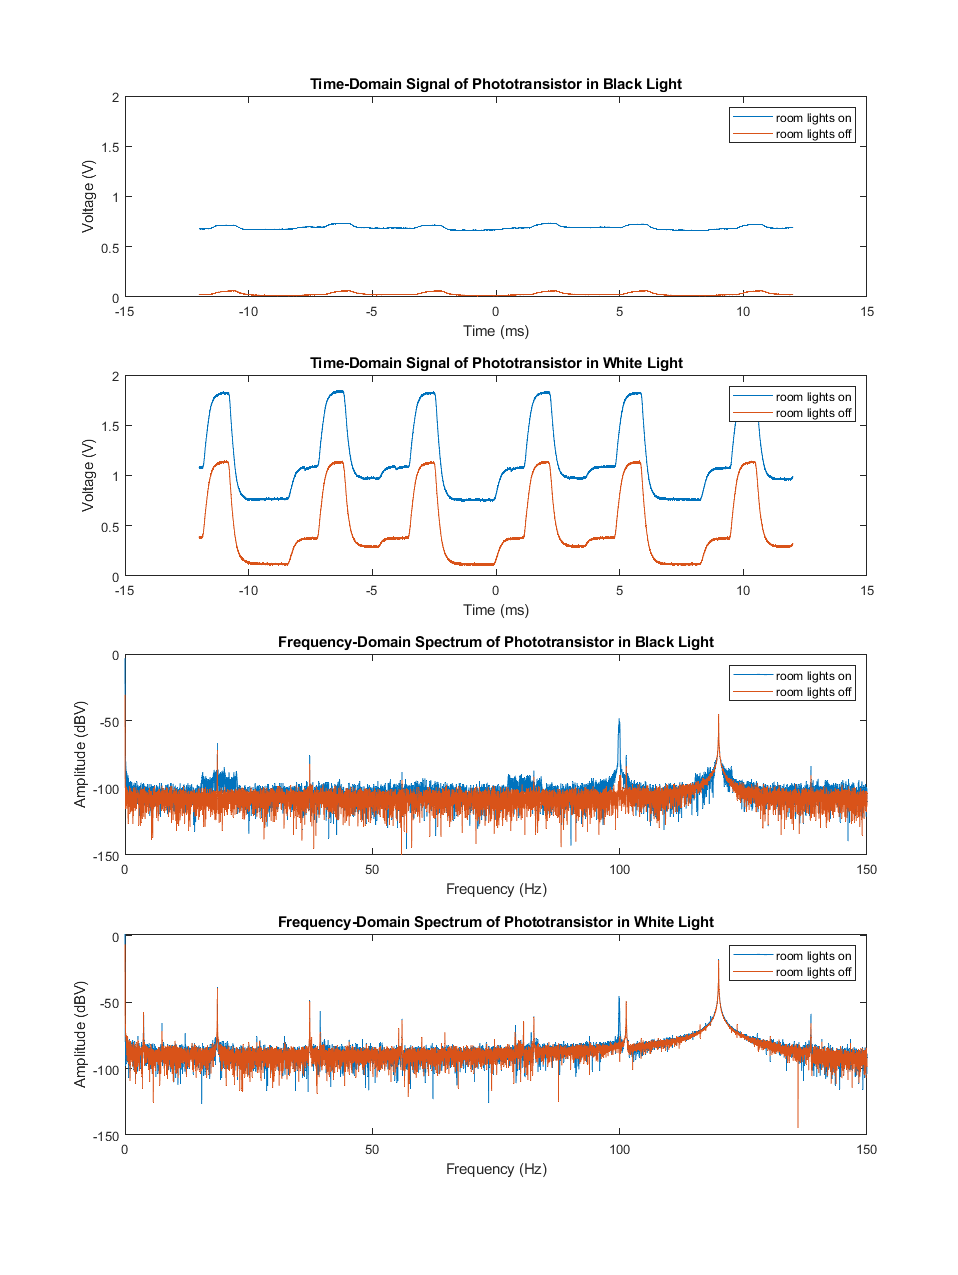
\includegraphics[width=0.5\textwidth]{sensor-matlab.png}}
% 	\caption{Selection of phototransistor time- and frequency-domain signals}
% 	\label{fig:sensor-matlab}
% \end{figure}

% \begin{figure}[htbp]
% 	\centerline{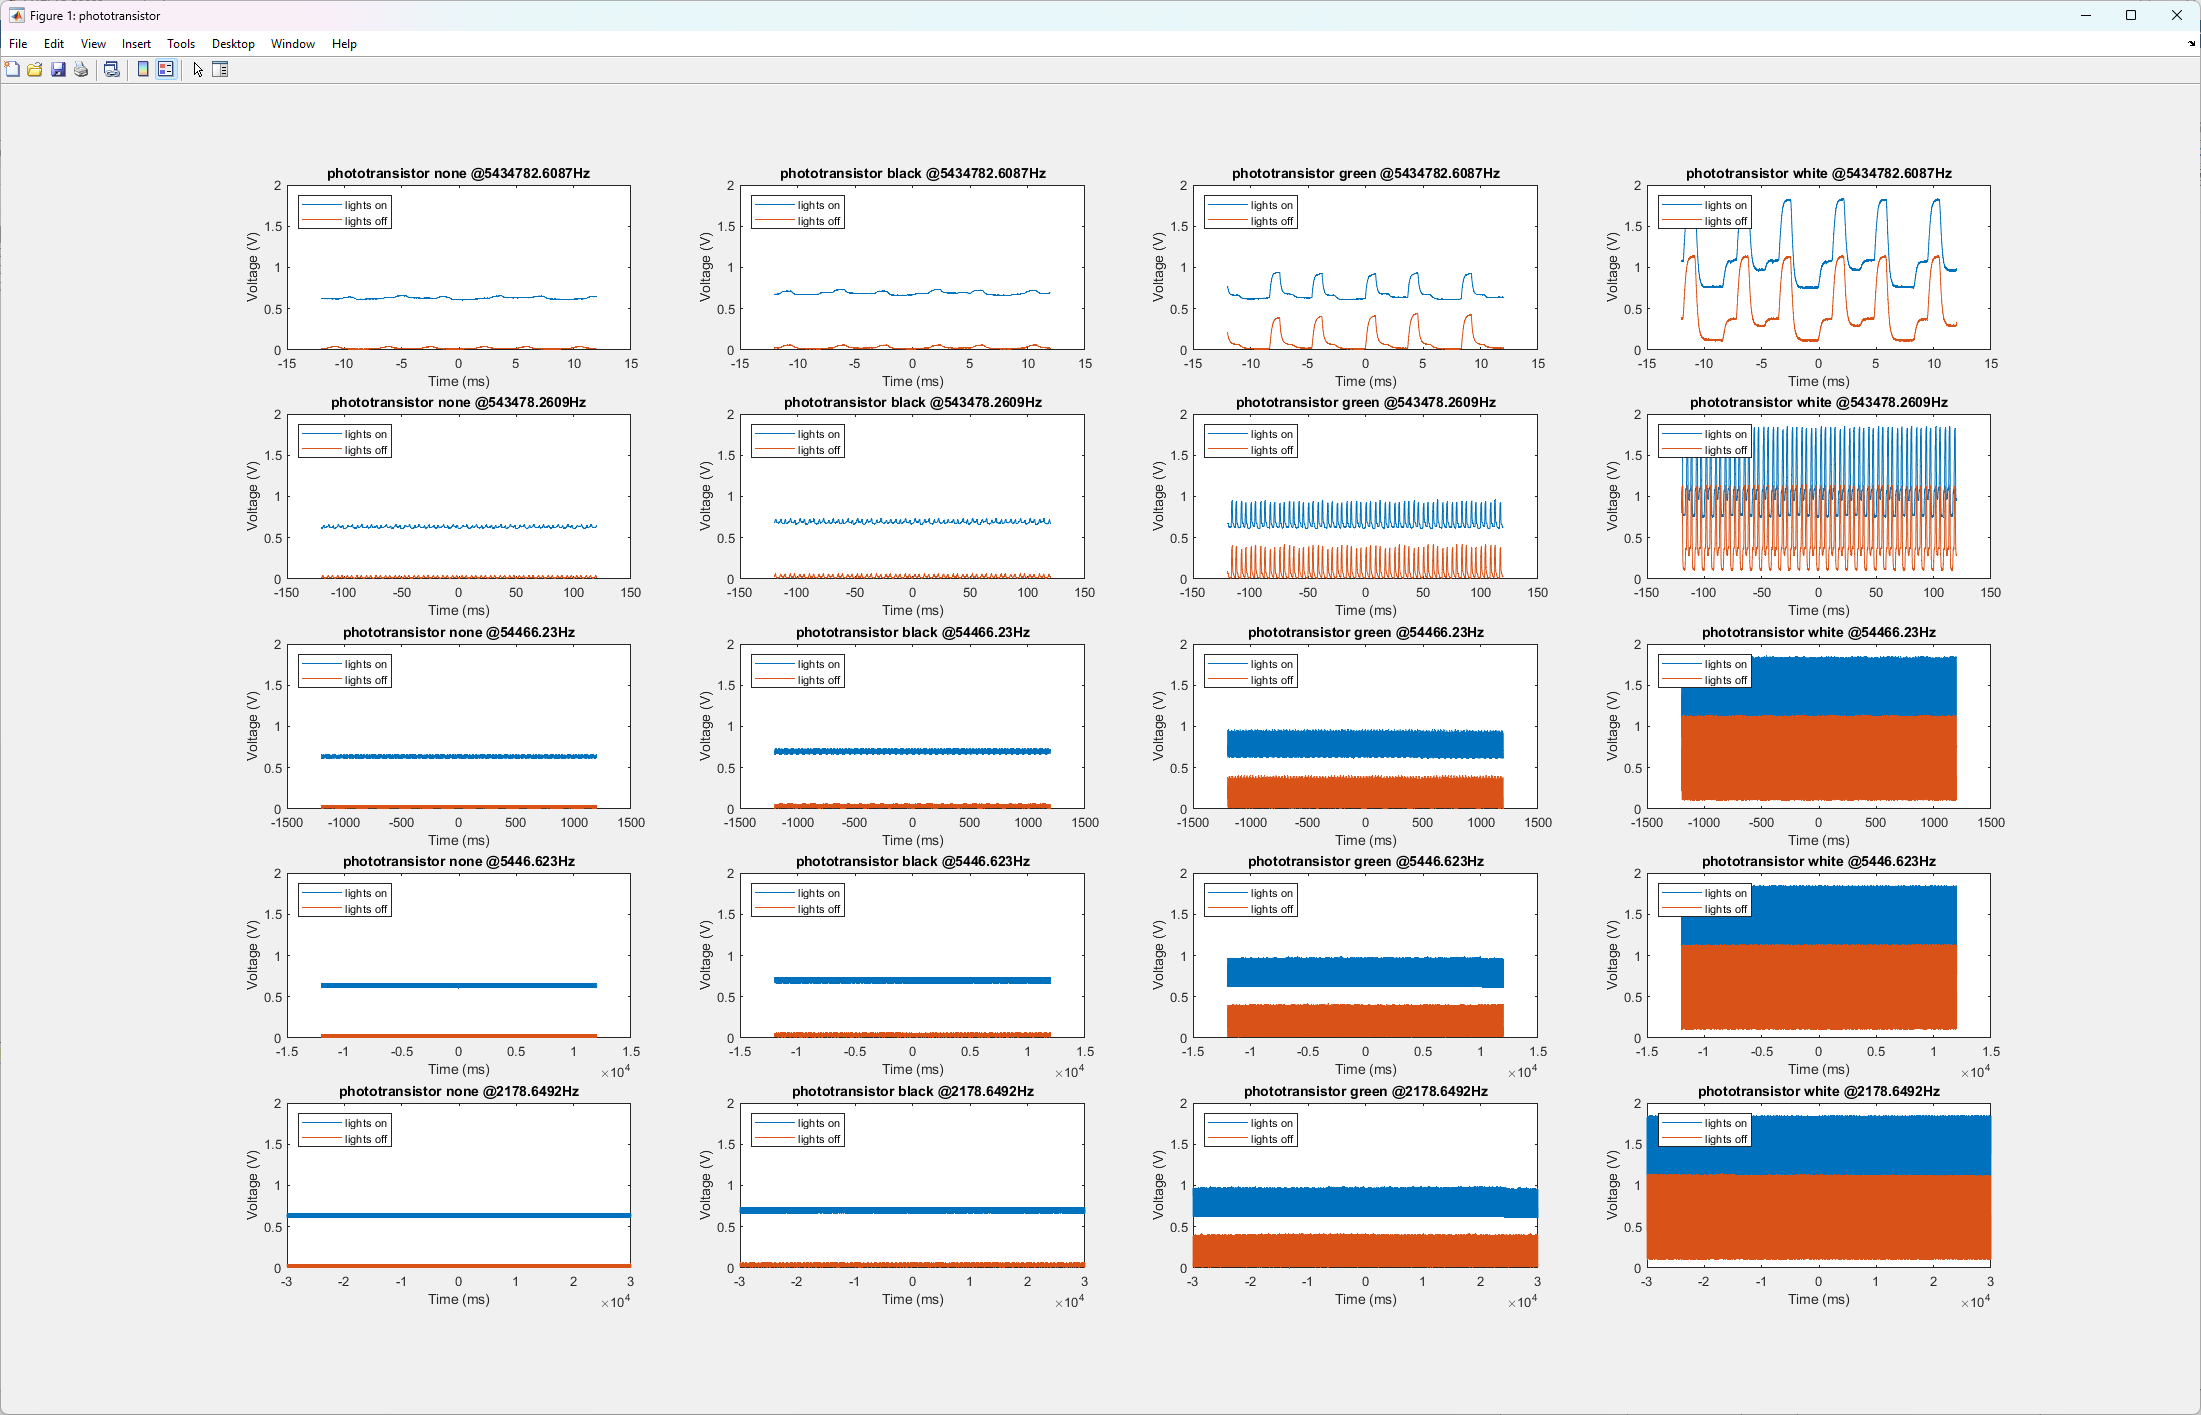
\includegraphics[width=0.5\textwidth]{phototransistor-time.png}}
% 	\caption{Time-domain phototransistor signals}
% 	\label{fig:phototransistor-time}
% \end{figure}
% \begin{figure}[htbp]
% 	\centerline{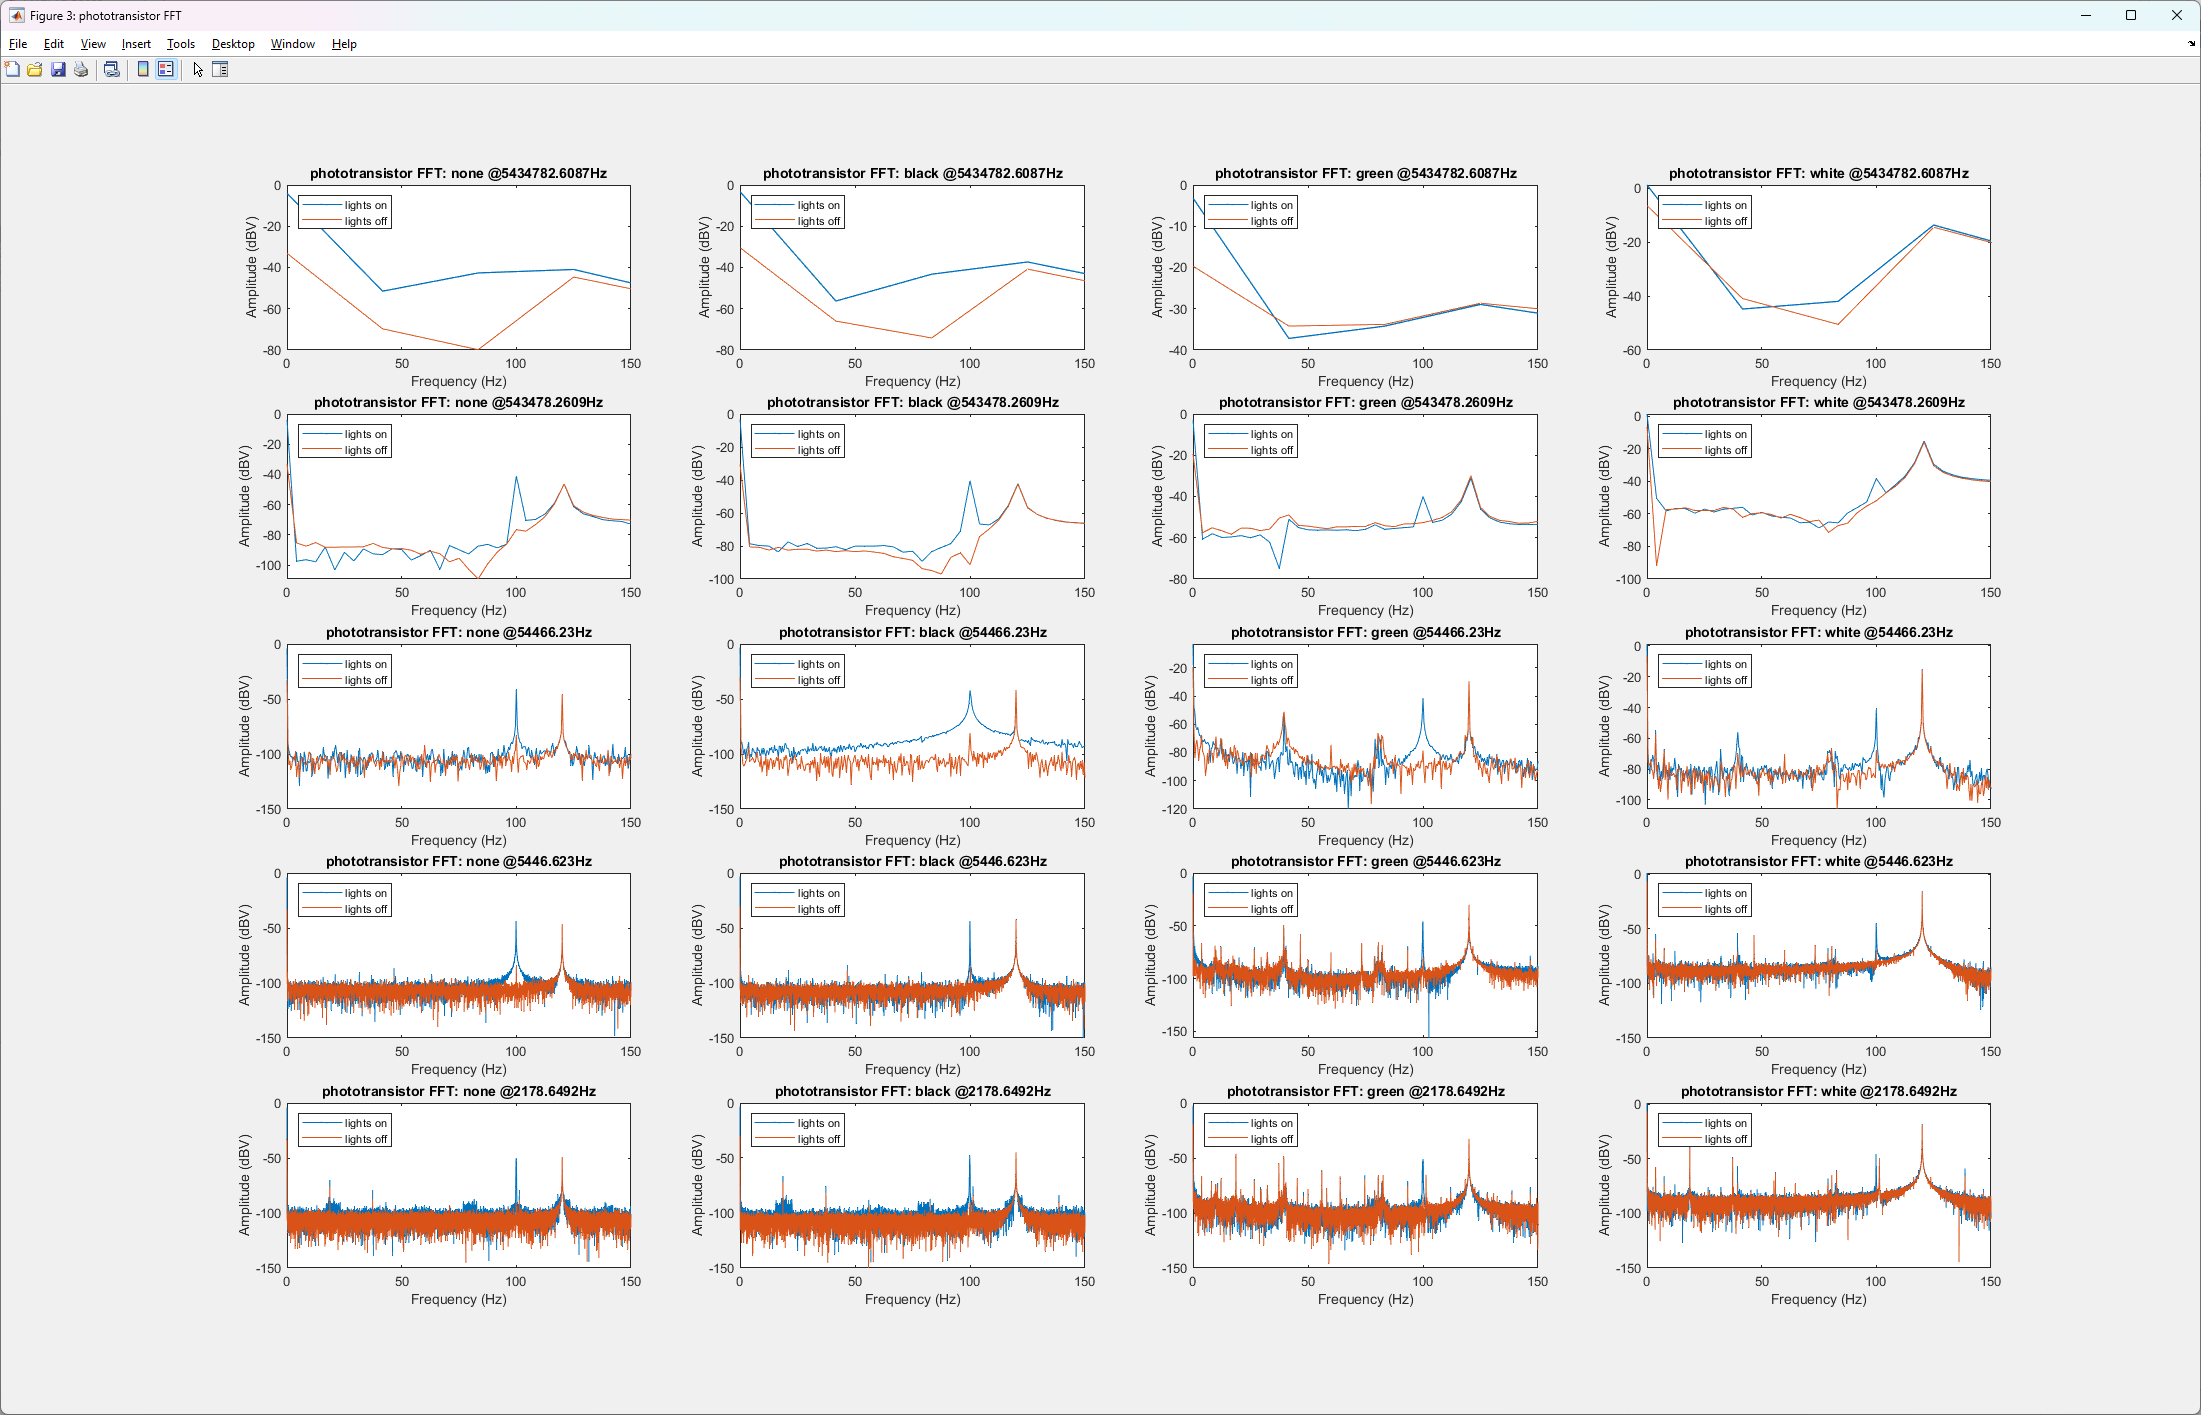
\includegraphics[width=0.5\textwidth]{phototransistor-frequency.png}}
% 	\caption{Frequency-domain phototransistor spectrums}
% 	\label{fig:phototransistor-frequency}
% \end{figure}
% \begin{figure}[htbp]
% 	\centerline{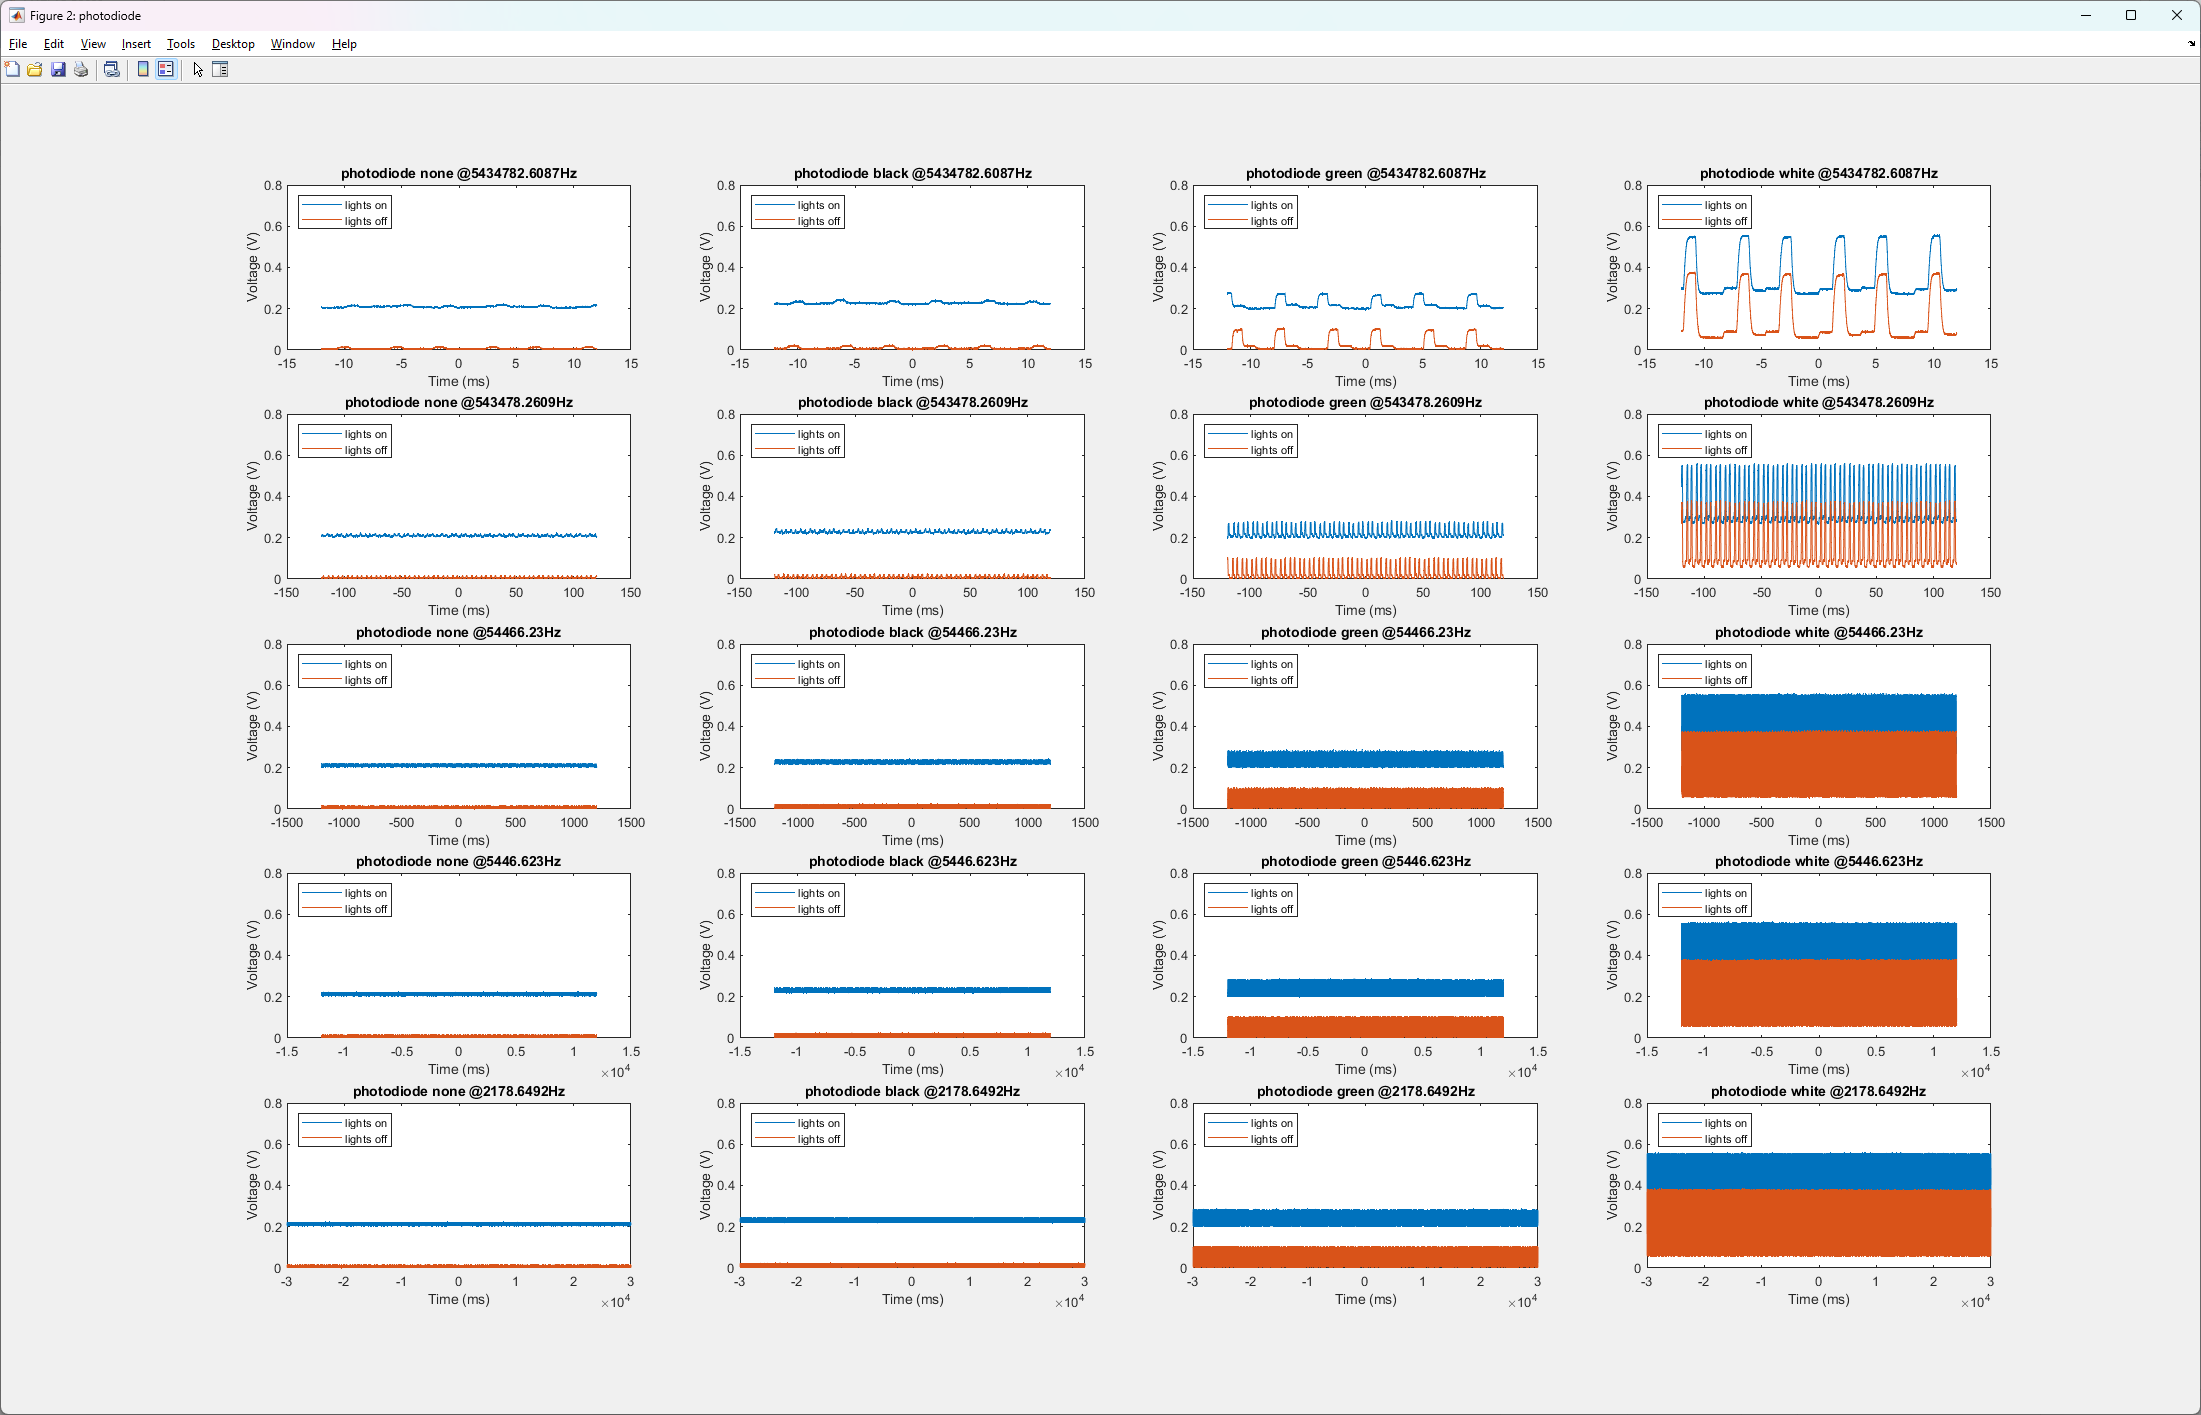
\includegraphics[width=0.5\textwidth]{photodiode-time.png}}
% 	\caption{Time-domain photodiode signals}
% 	\label{fig:photodiode-time}
% \end{figure}
% \begin{figure}[htbp]
% 	\centerline{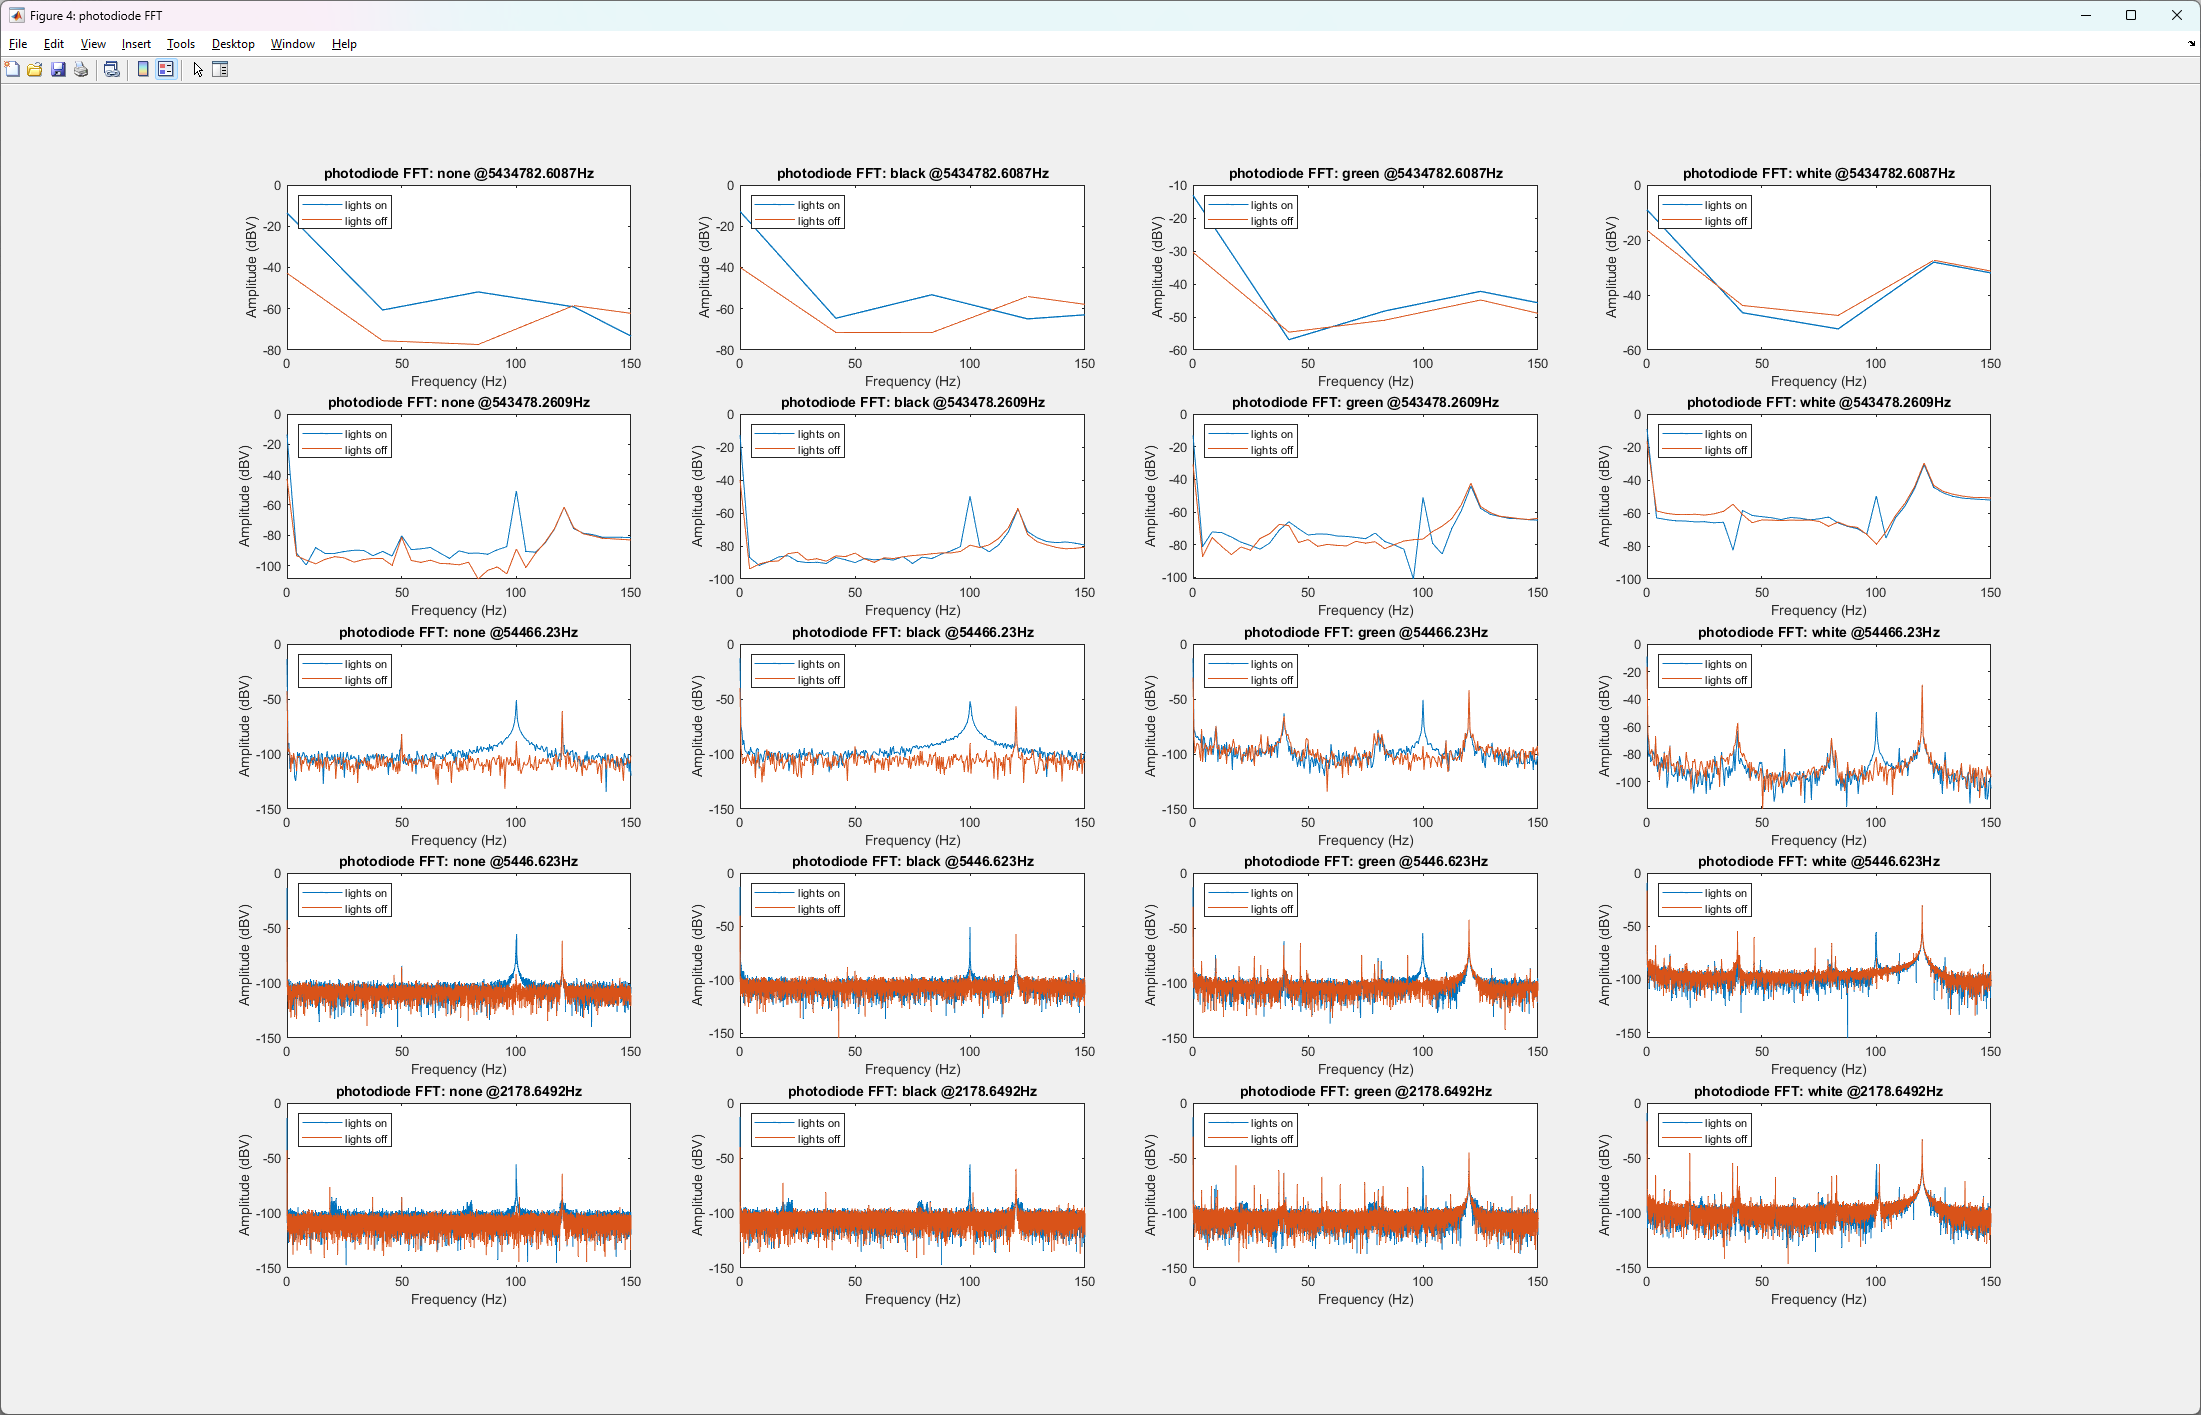
\includegraphics[width=0.5\textwidth]{photodiode-frequency.png}}
% 	\caption{Frequency-domain photodiode spectrums}
% 	\label{fig:photodiode-frequency}
% \end{figure}
% \begin{figure}[htbp]
% 	\centerline{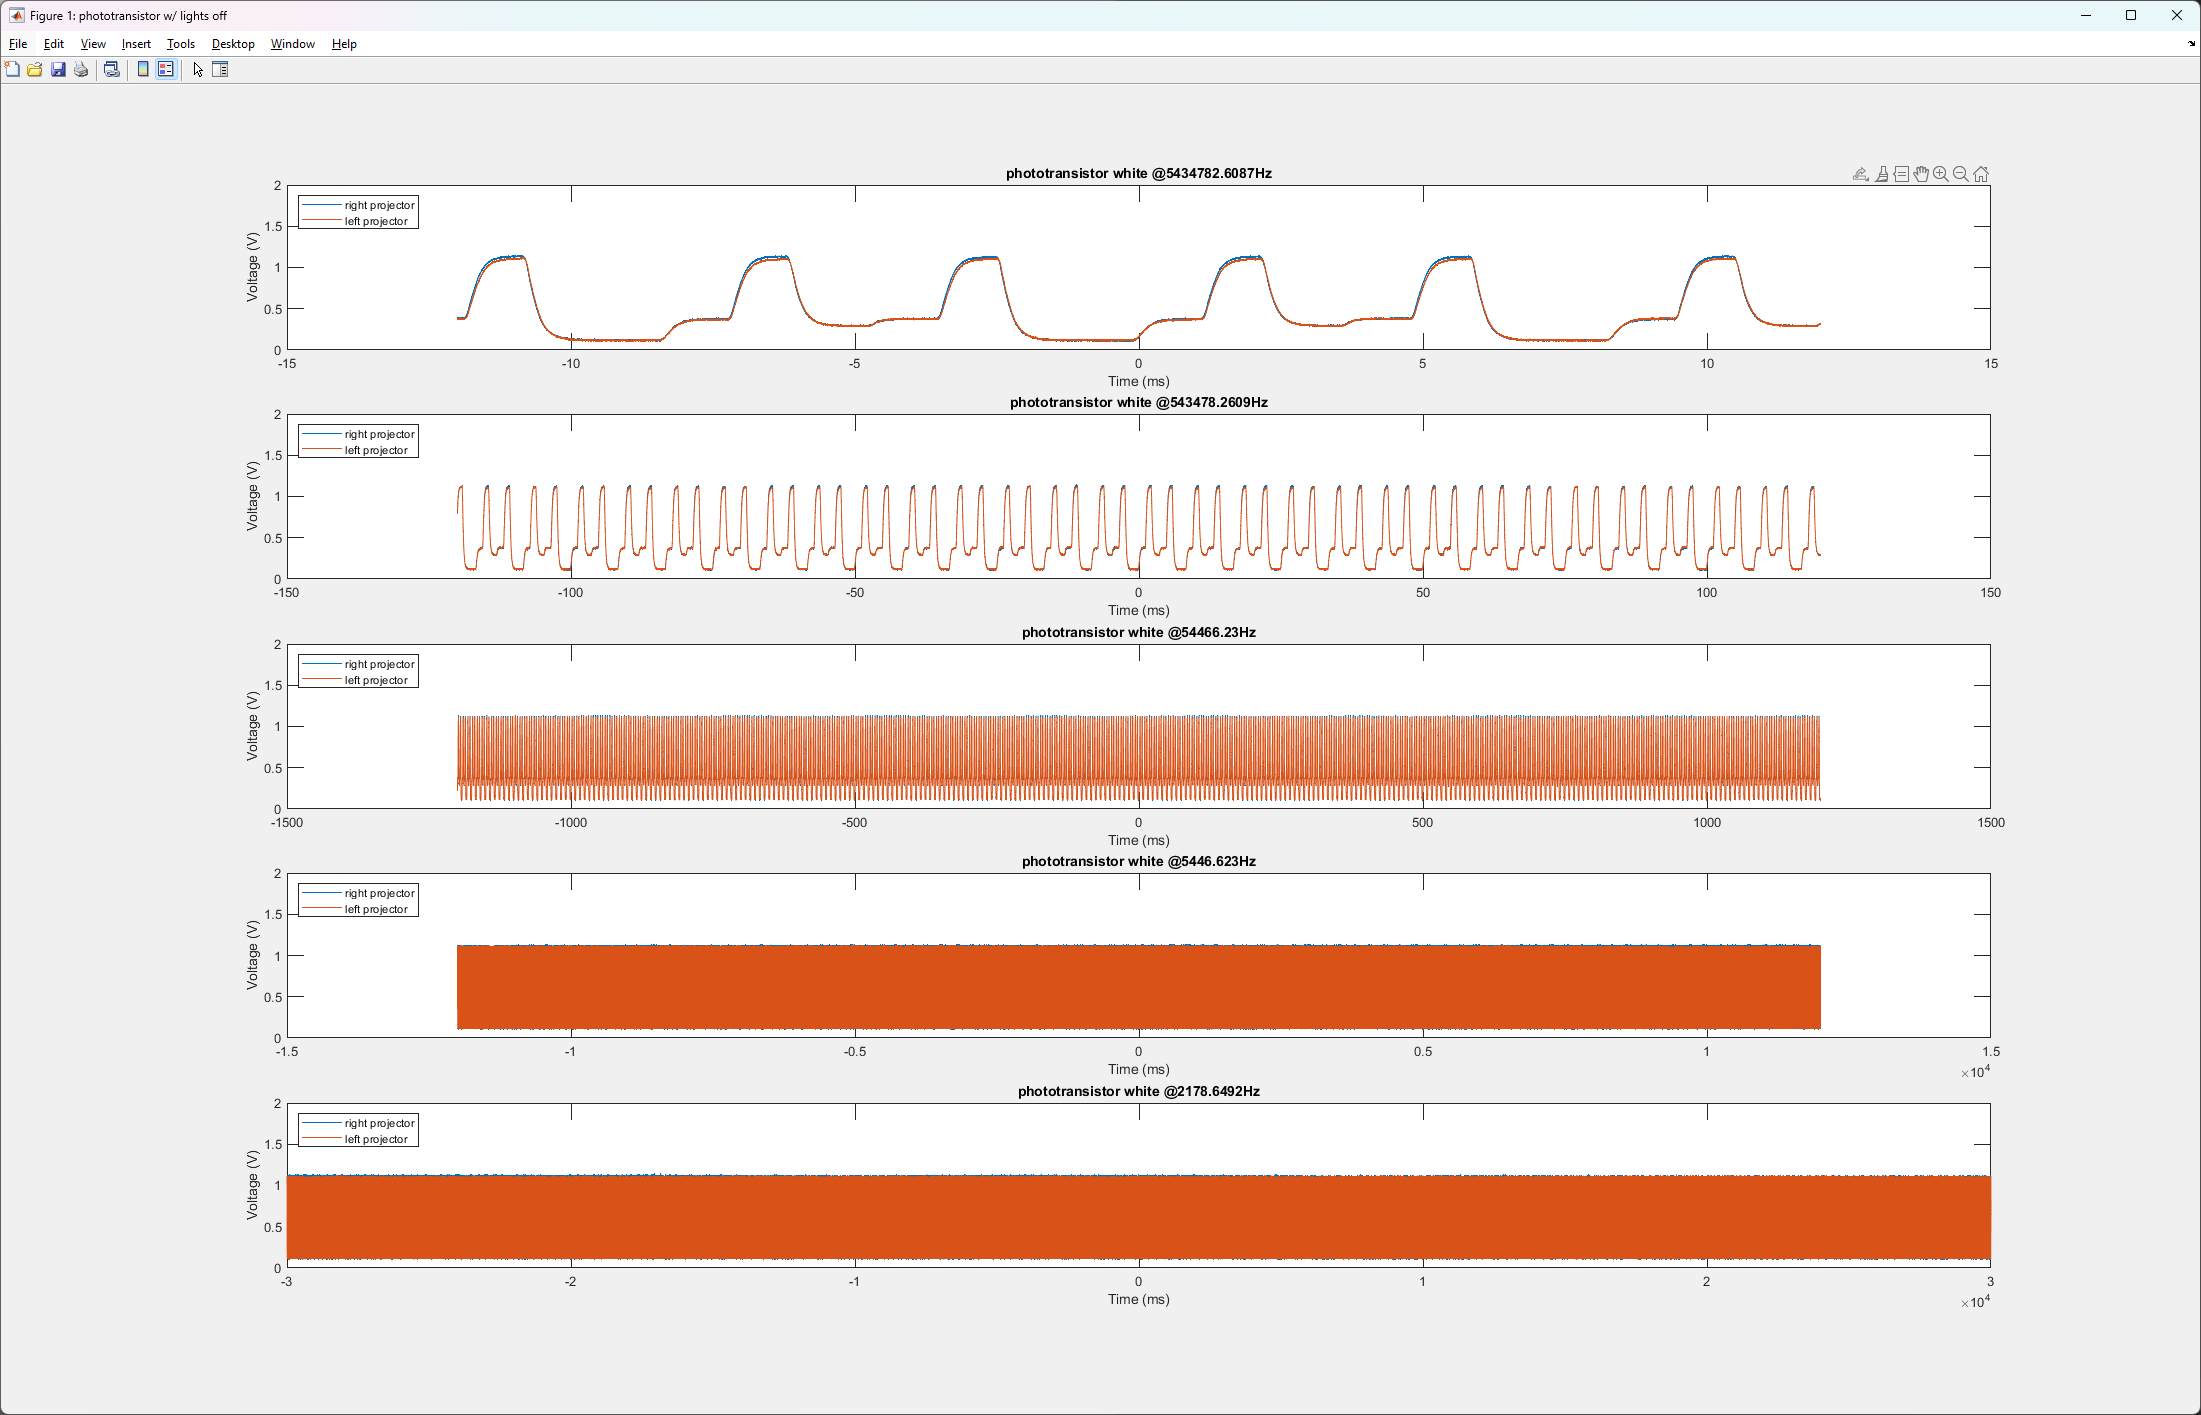
\includegraphics[width=0.5\textwidth]{projector-phototransistor-time.png}}
% 	\caption{Time-domain phototransistor signal comparison between projectors}
% 	\label{fig:projector-phototransistor-time}
% \end{figure}
% \begin{figure}[htbp]
% 	\centerline{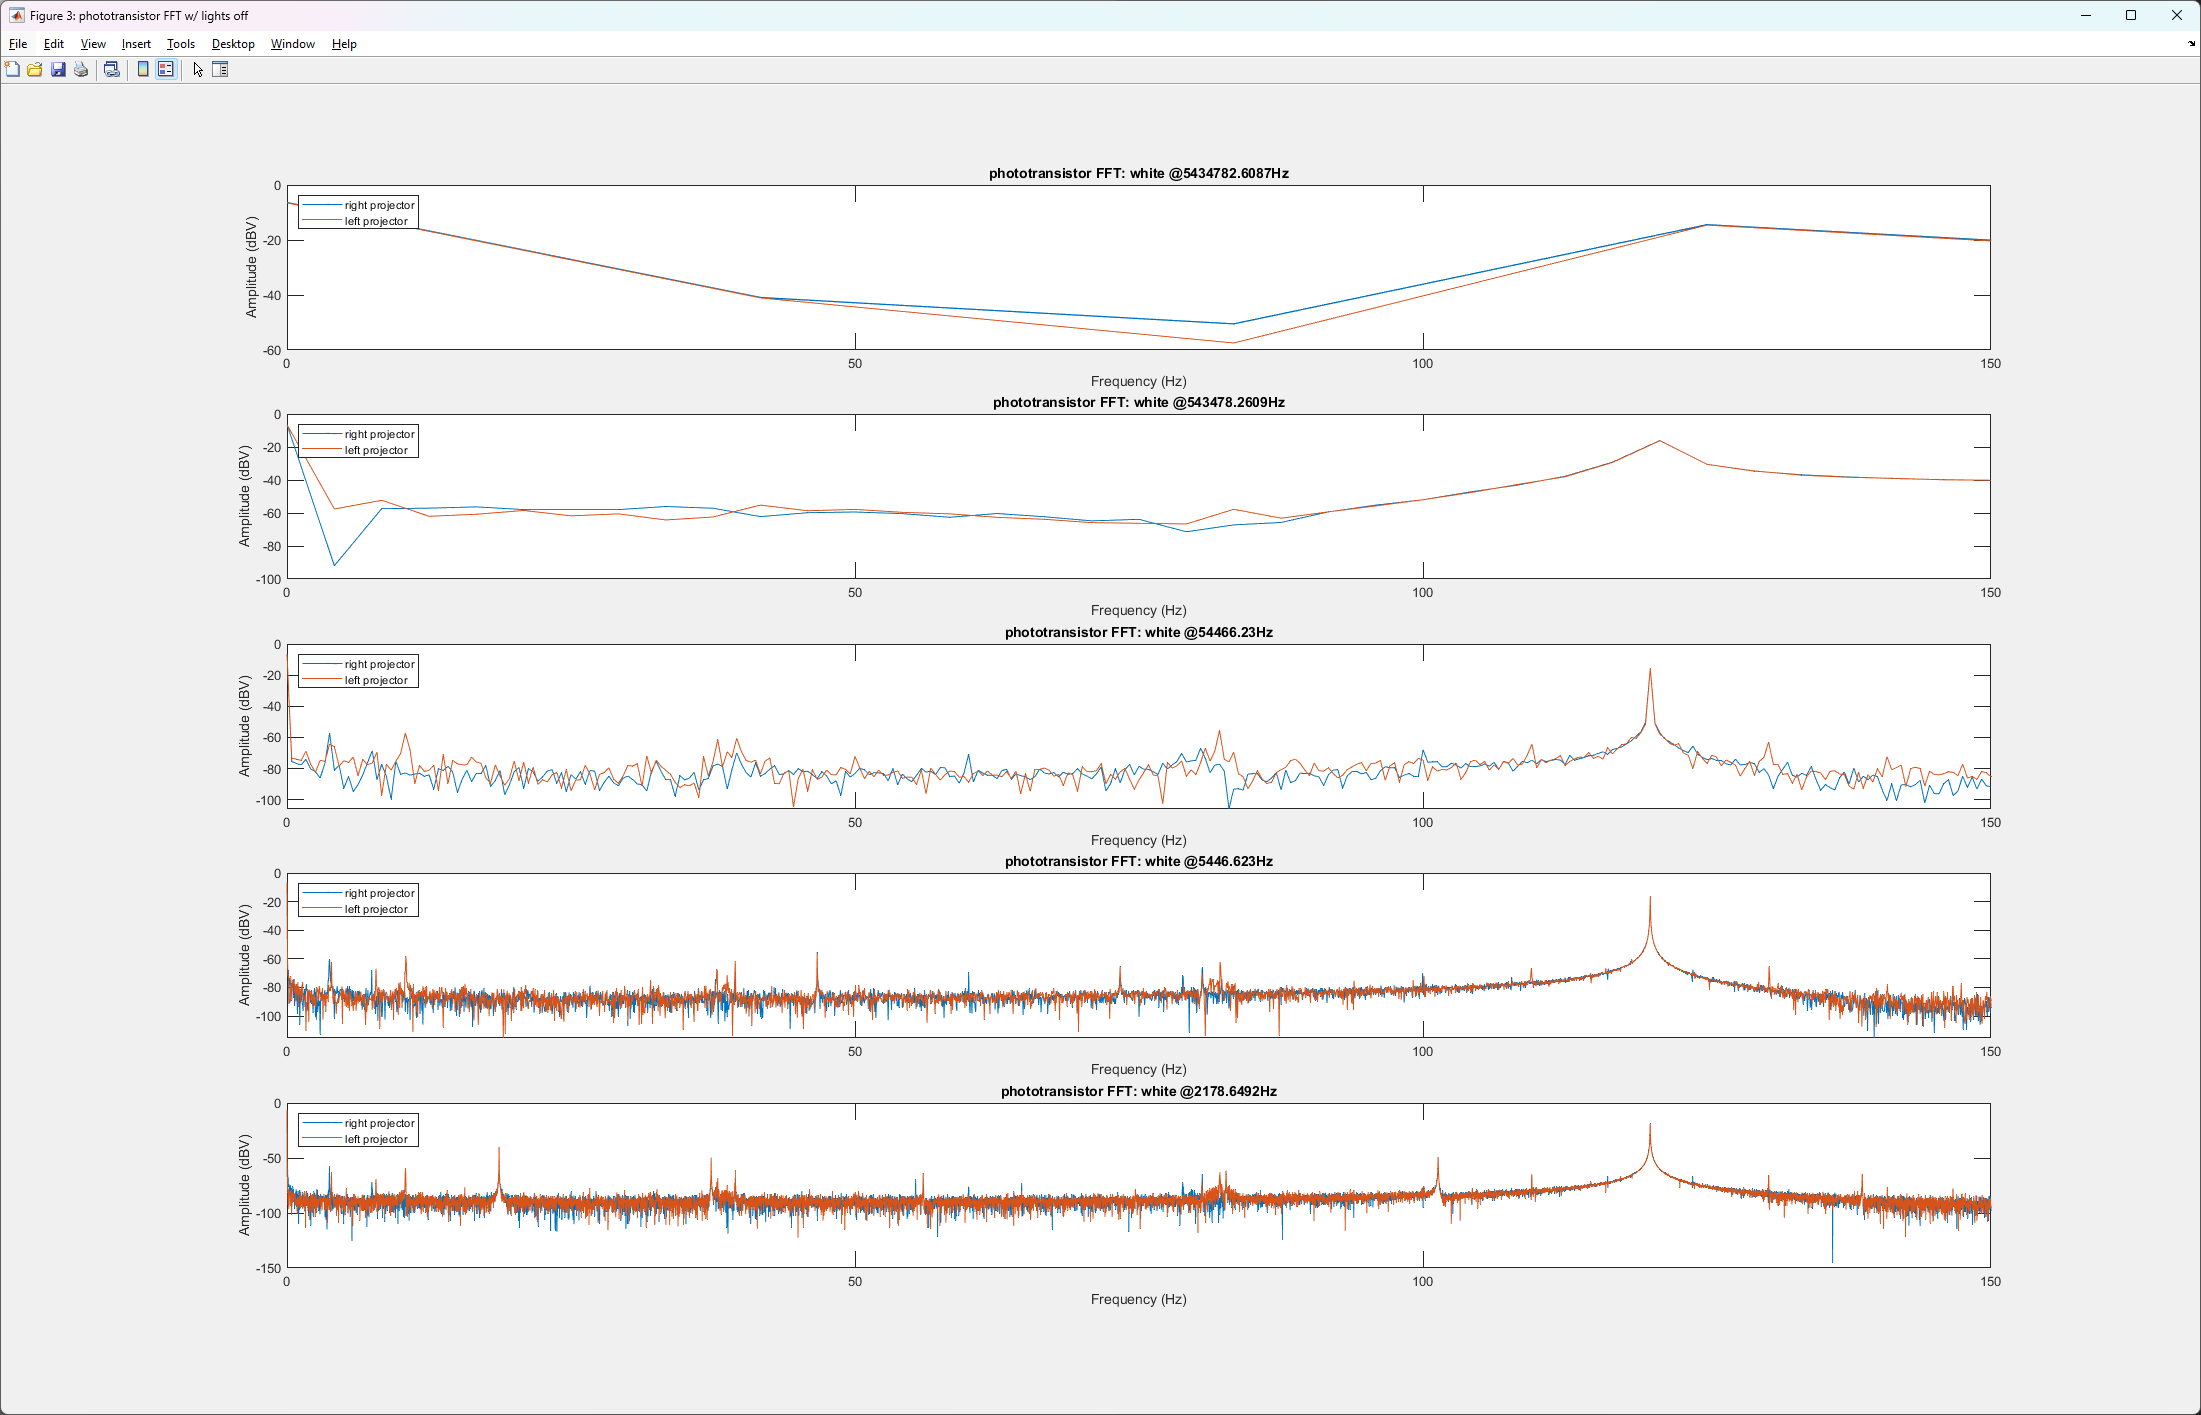
\includegraphics[width=0.5\textwidth]{projector-phototransistor-frequency.png}}
% 	\caption{Frequency-domain phototransistor spectrum comparison between projectors}
% 	\label{fig:projector-phototransistor-frequency}
% \end{figure}
% \begin{figure}[htbp]
% 	\centerline{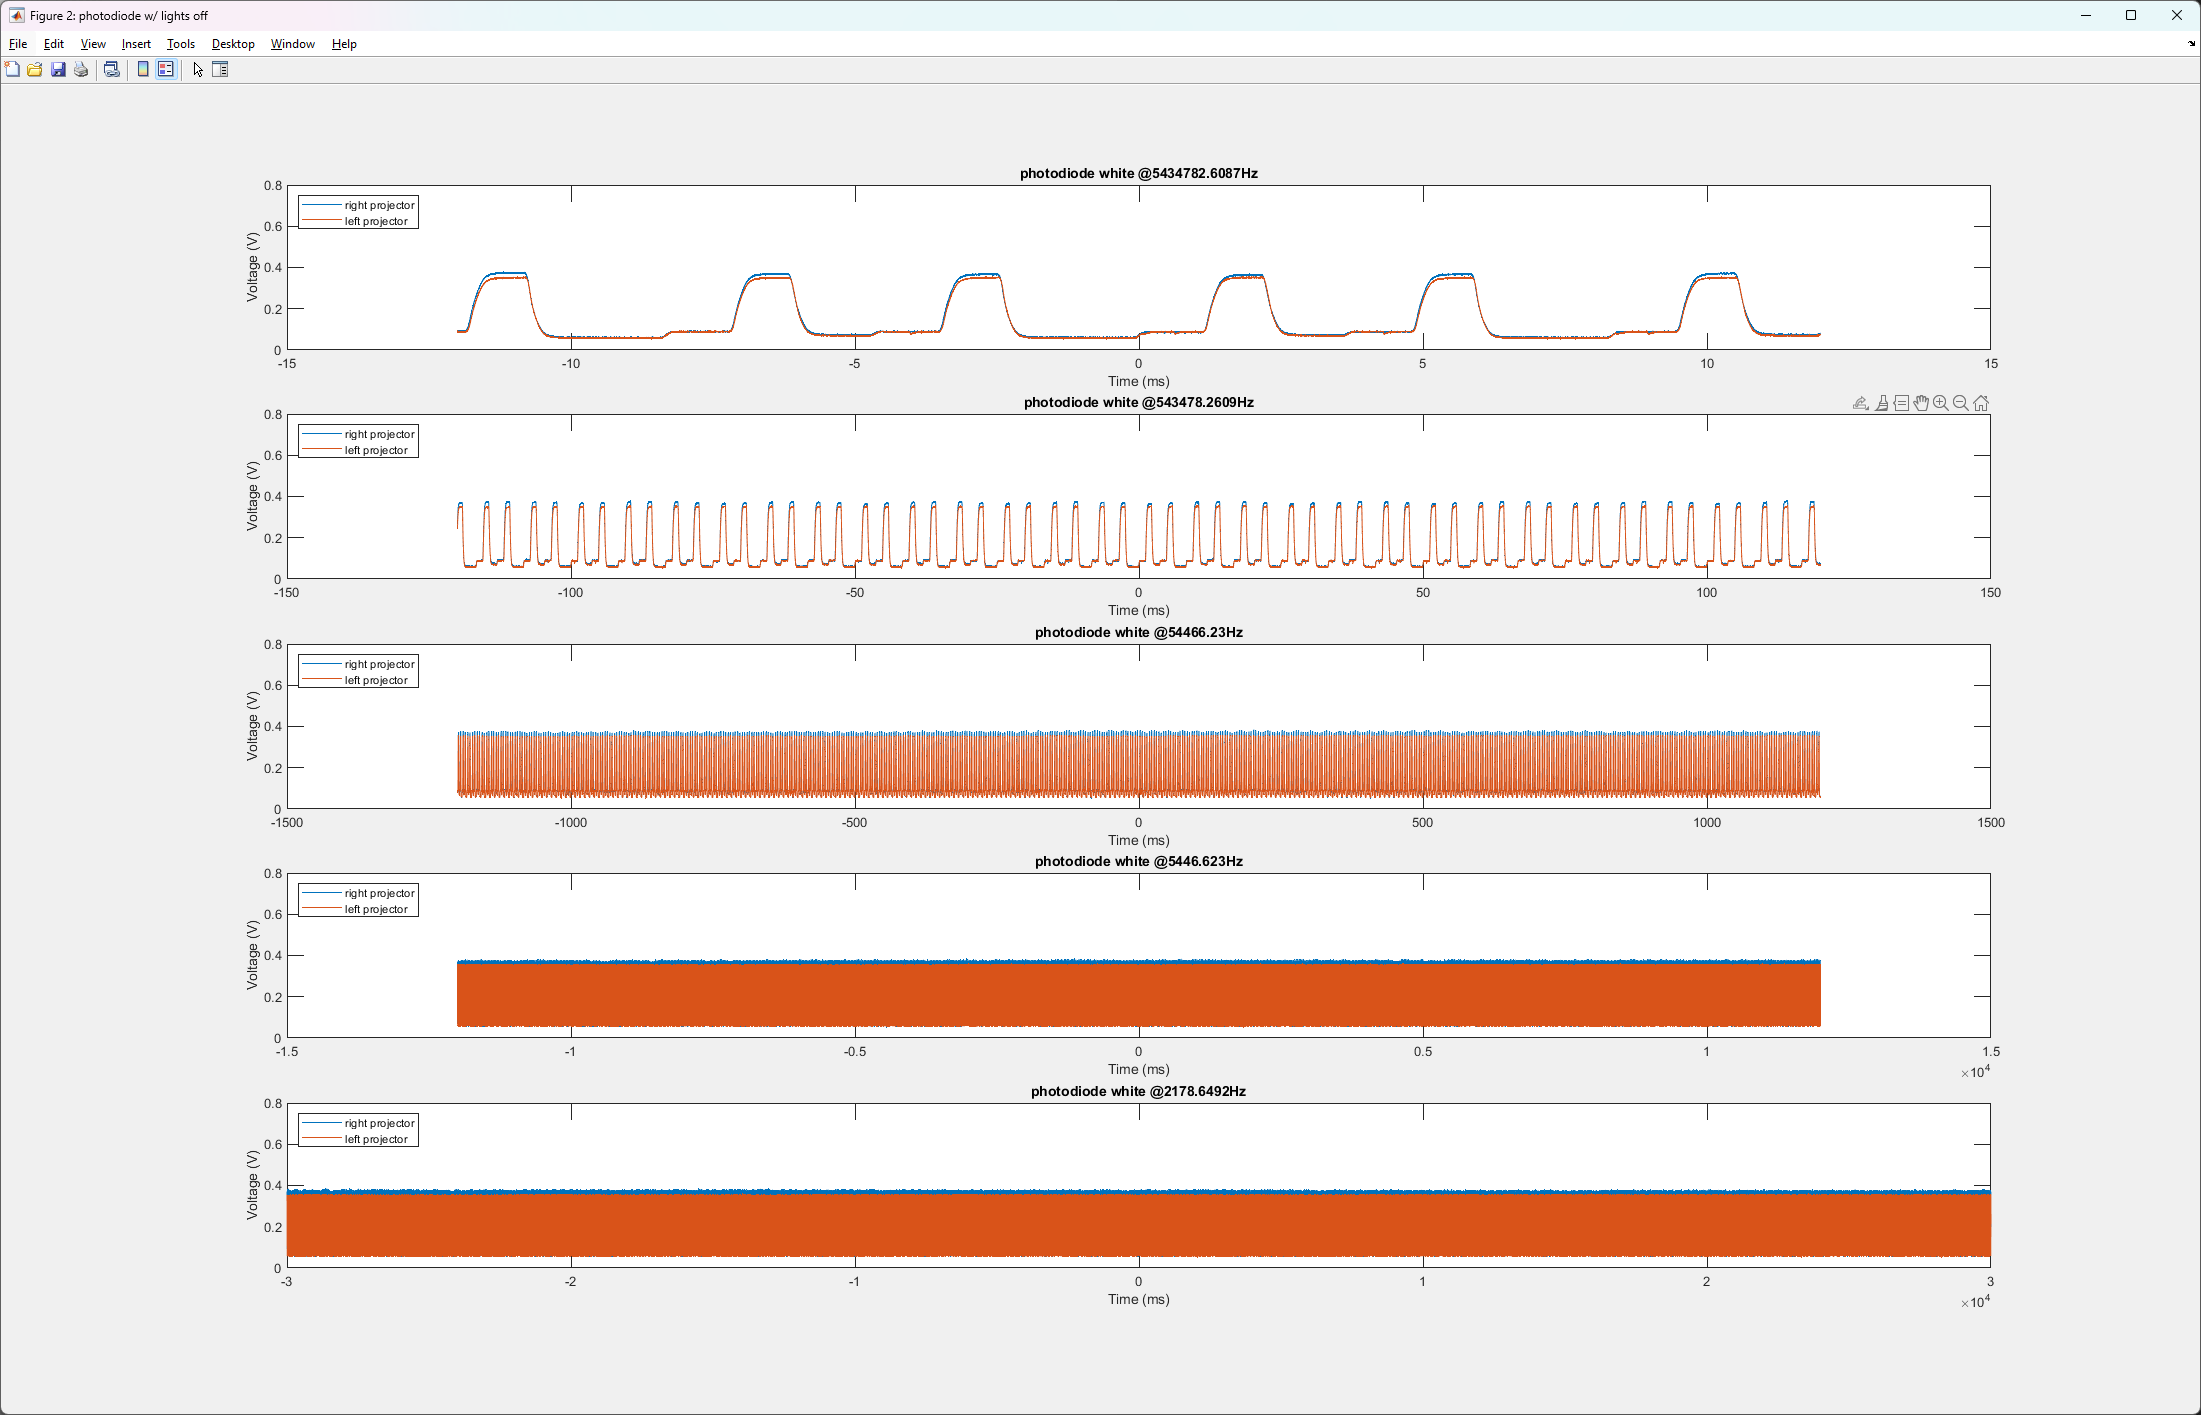
\includegraphics[width=0.5\textwidth]{projector-photodiode-time.png}}
% 	\caption{Time-domain photodiode signal comparison between projectors}
% 	\label{fig:projector-photodiode-time}
% \end{figure}
% \begin{figure}[htbp]
% 	\centerline{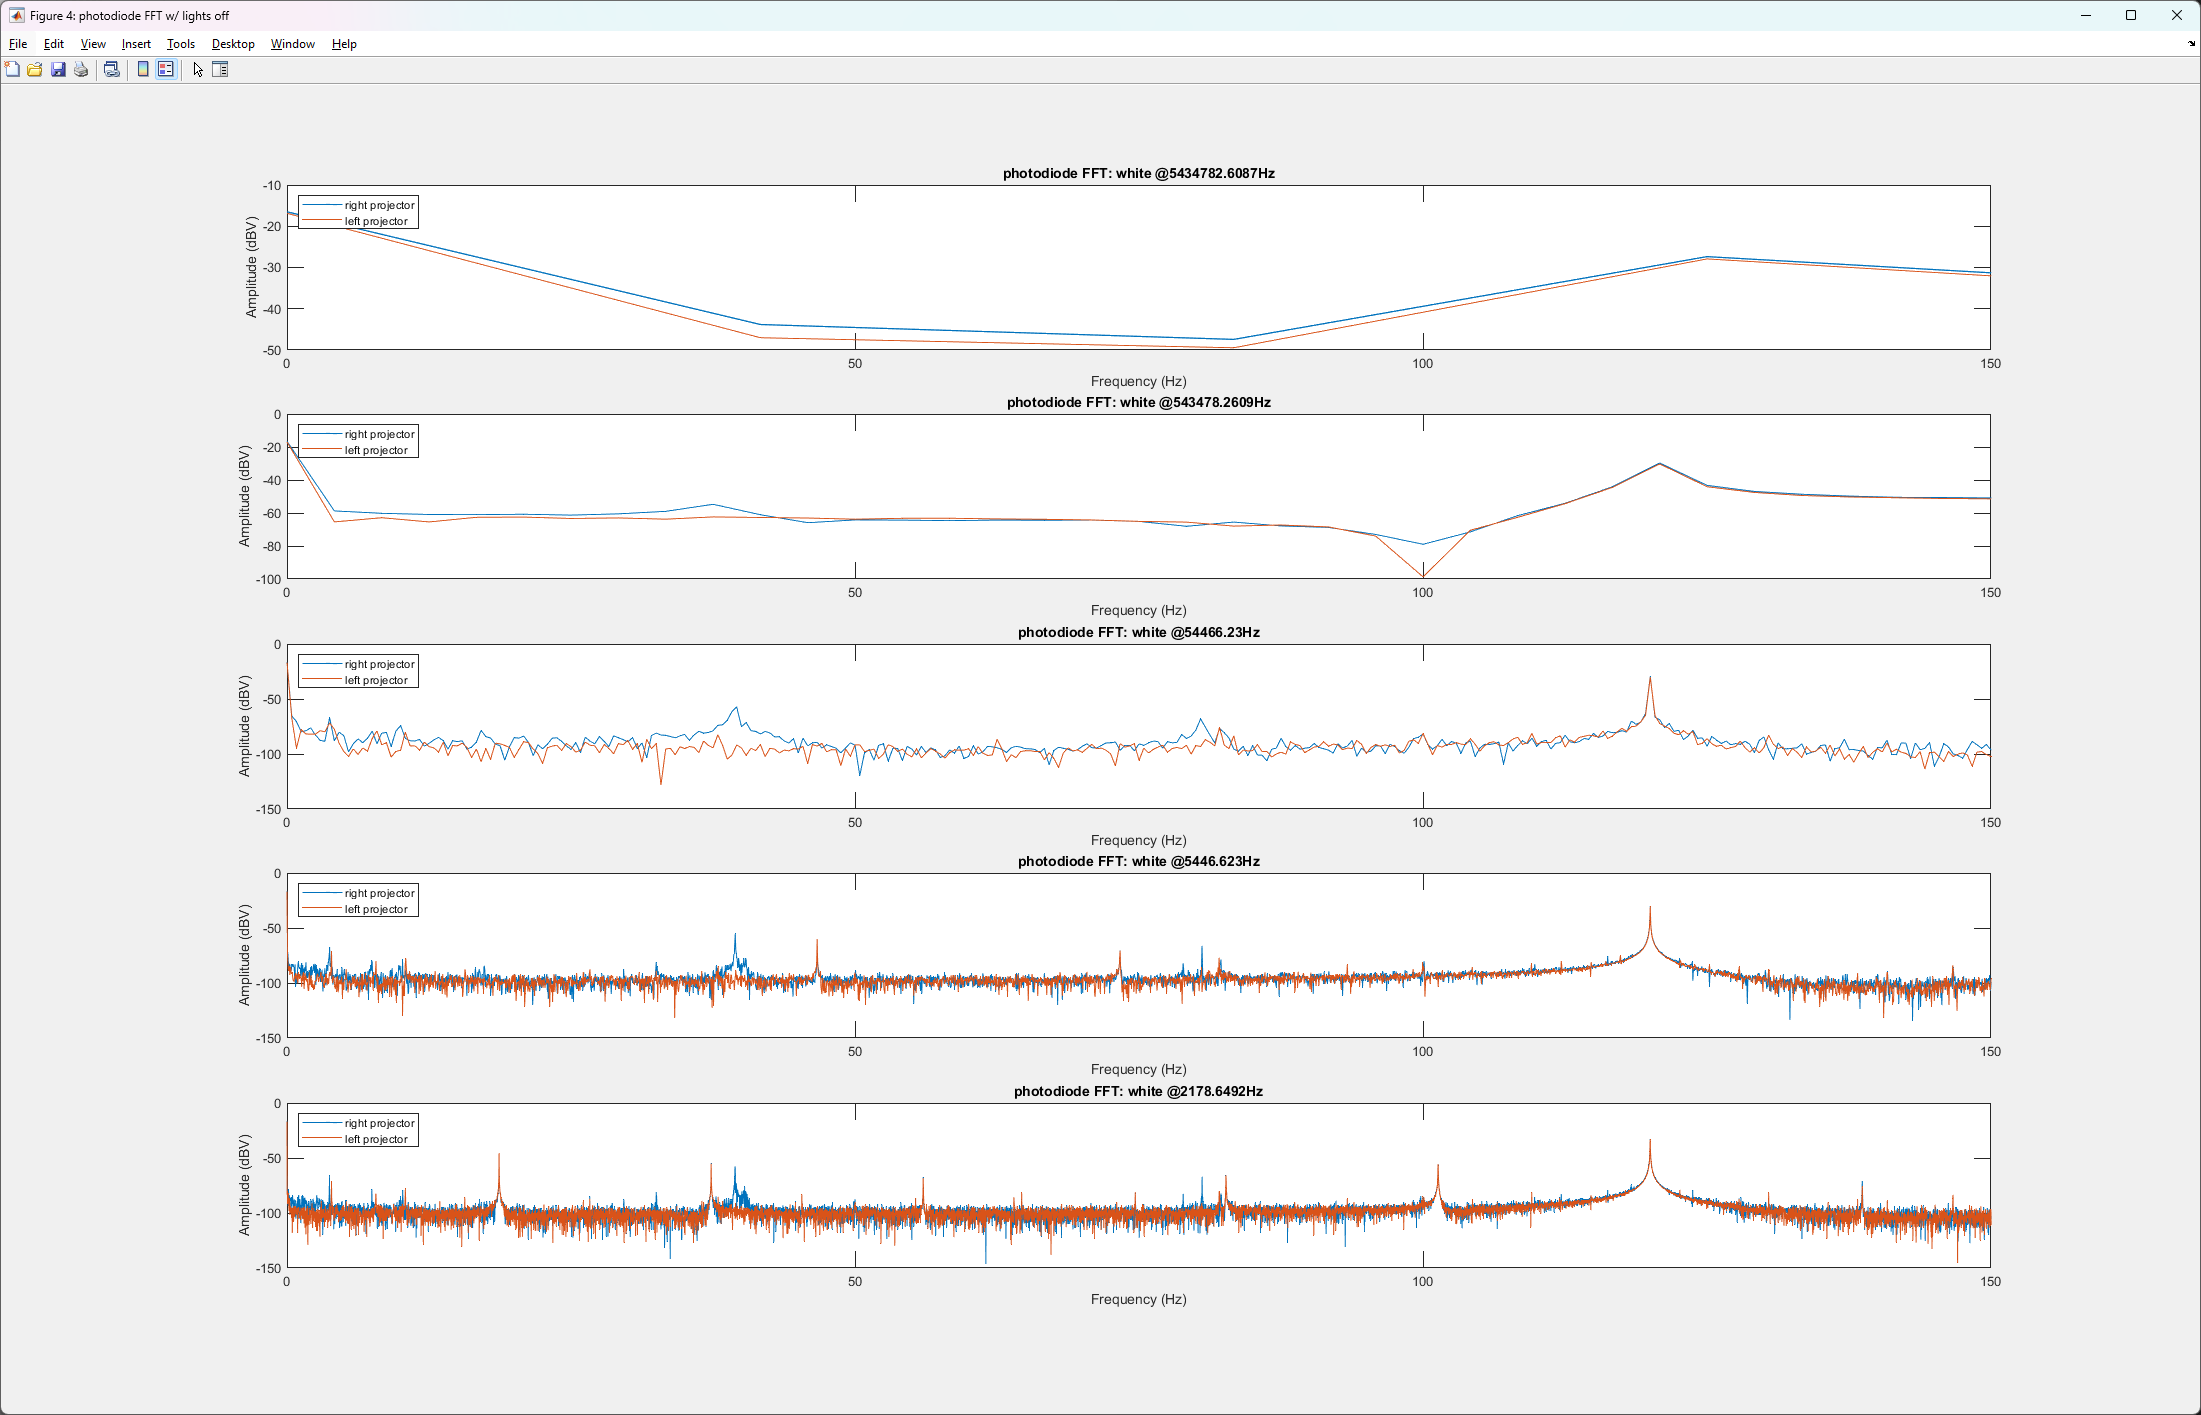
\includegraphics[width=0.5\textwidth]{projector-photodiode-frequency.png}}
% 	\caption{Frequency-domain photodiode spectrum comparison between projectors}
% 	\label{fig:projector-photodiode-frequency}
% \end{figure}

% \begin{figure}[htbp]
% 	\centerline{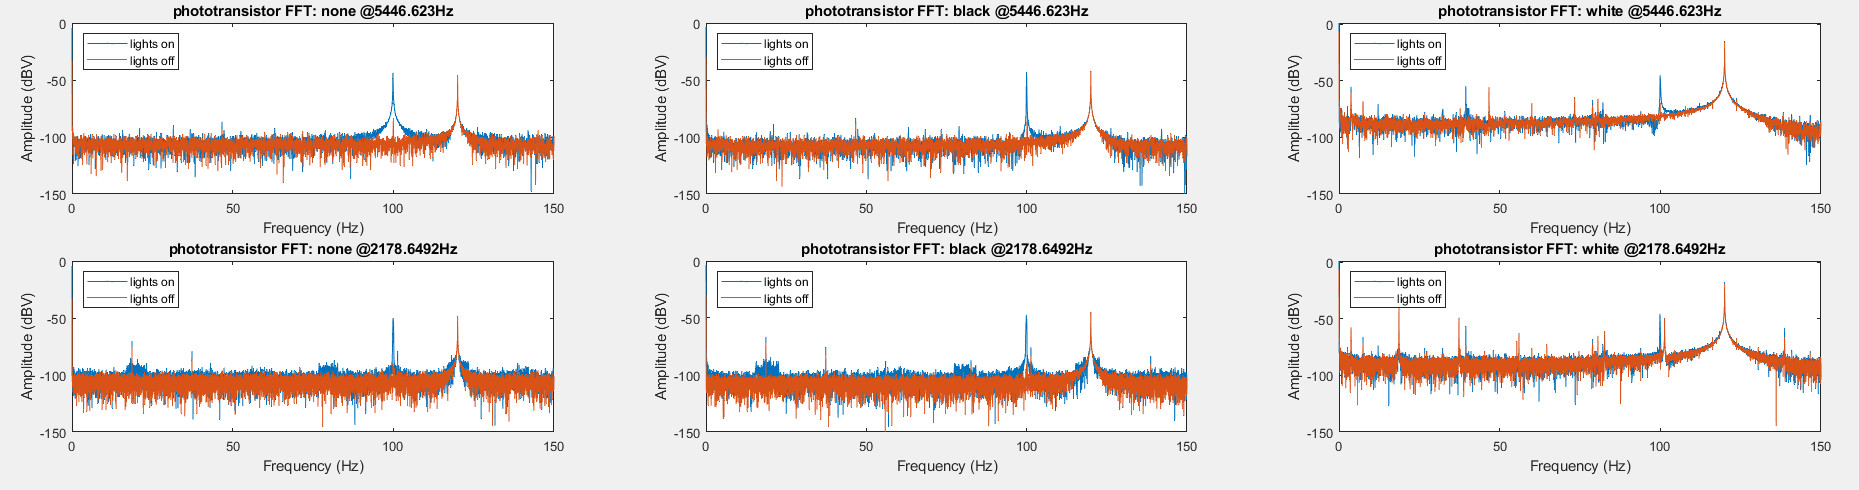
\includegraphics[width=0.5\textwidth]{sensor-phototransistor-sensitivity.png}}
% 	\caption{Frequency-domain phototransistor spectrum comparison between ambient lights on/off}
% 	\label{fig:sensor-phototransistor-sensitivity}
% \end{figure}
% \begin{figure}[htbp]
% 	\centerline{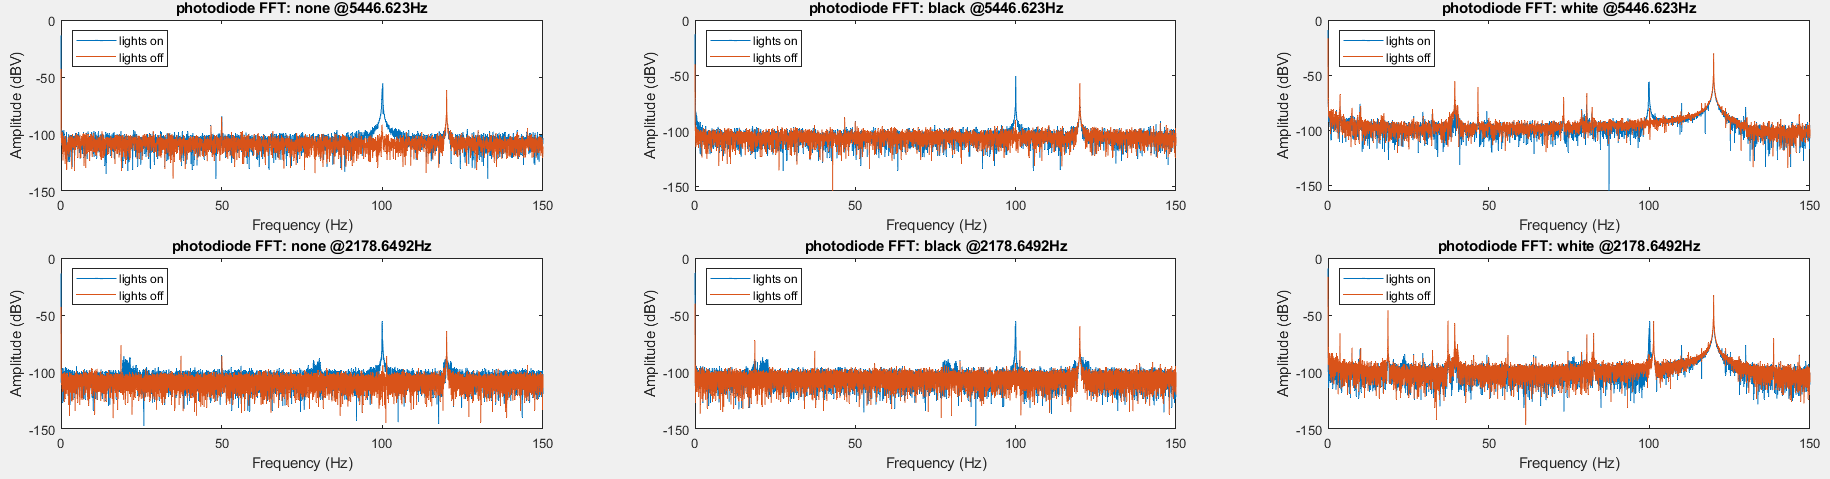
\includegraphics[width=0.5\textwidth]{sensor-photodiode-sensitivity.png}}
% 	\caption{Frequency-domain photodiode spectrum comparison between ambient lights on/off}
% 	\label{fig:sensor-photodiode-sensitivity}
% \end{figure}

% \subsection{Analogue Circuitry Design}

% \begin{figure}[htbp]
% 	\centerline{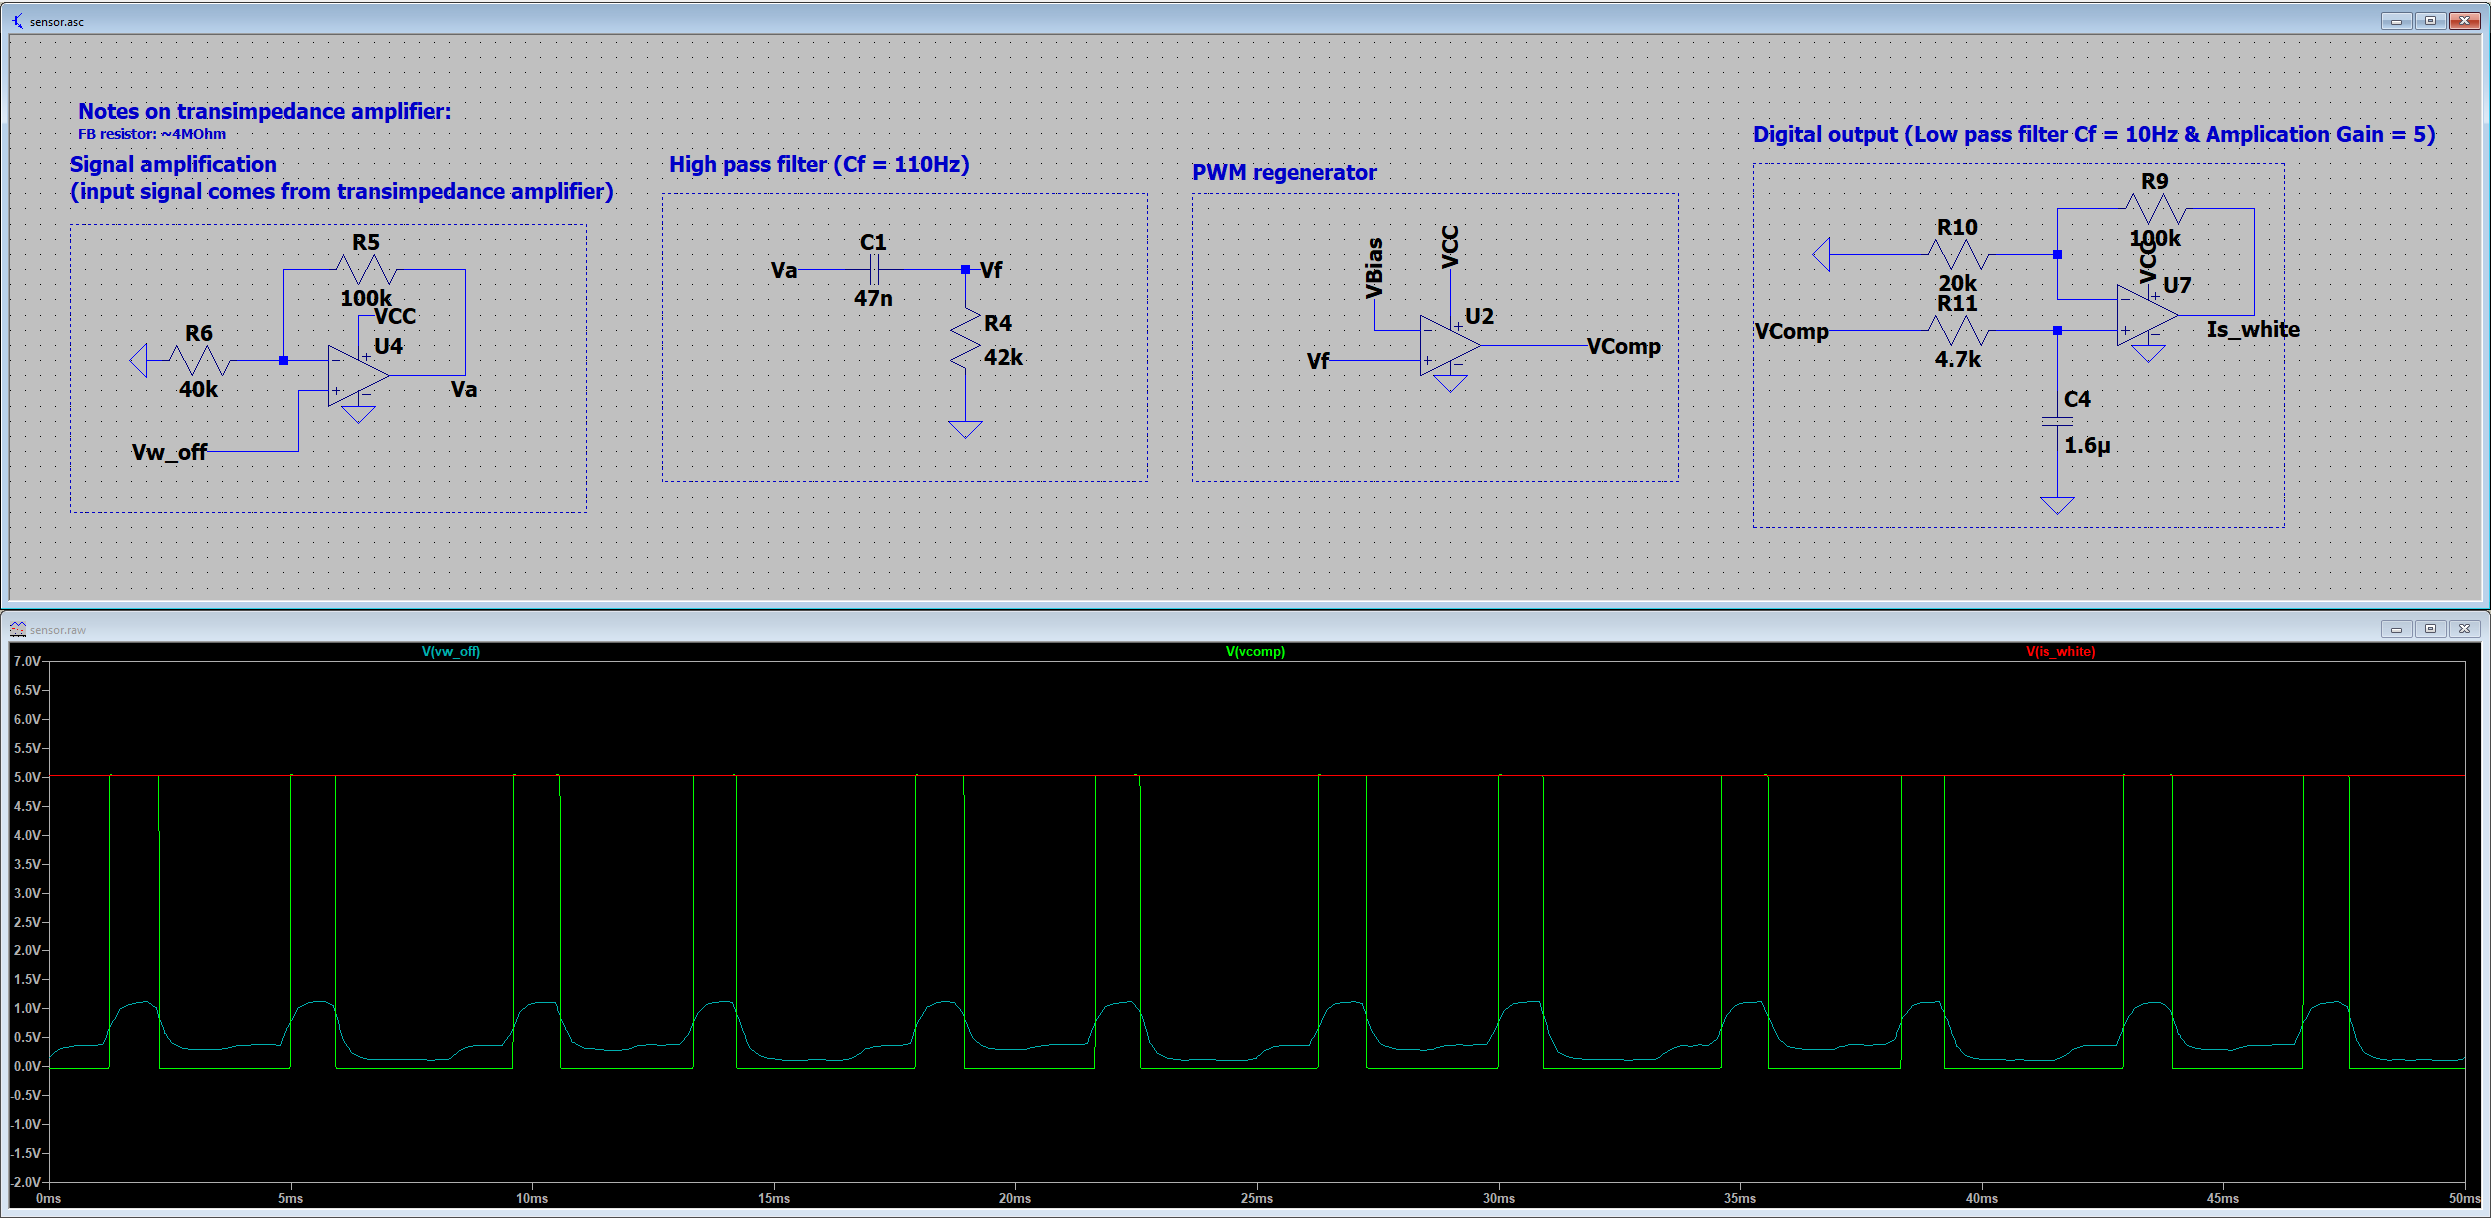
\includegraphics[width=0.5\textwidth]{sensor-spice.png}}
% 	\caption{Simulation of our sensor circuitry in \texttt{LTspice}}
% 	\label{fig:sensor-spice}
% \end{figure}

% \subsection{Constellation Design}

% \begin{figure}[htbp]
% 	\centerline{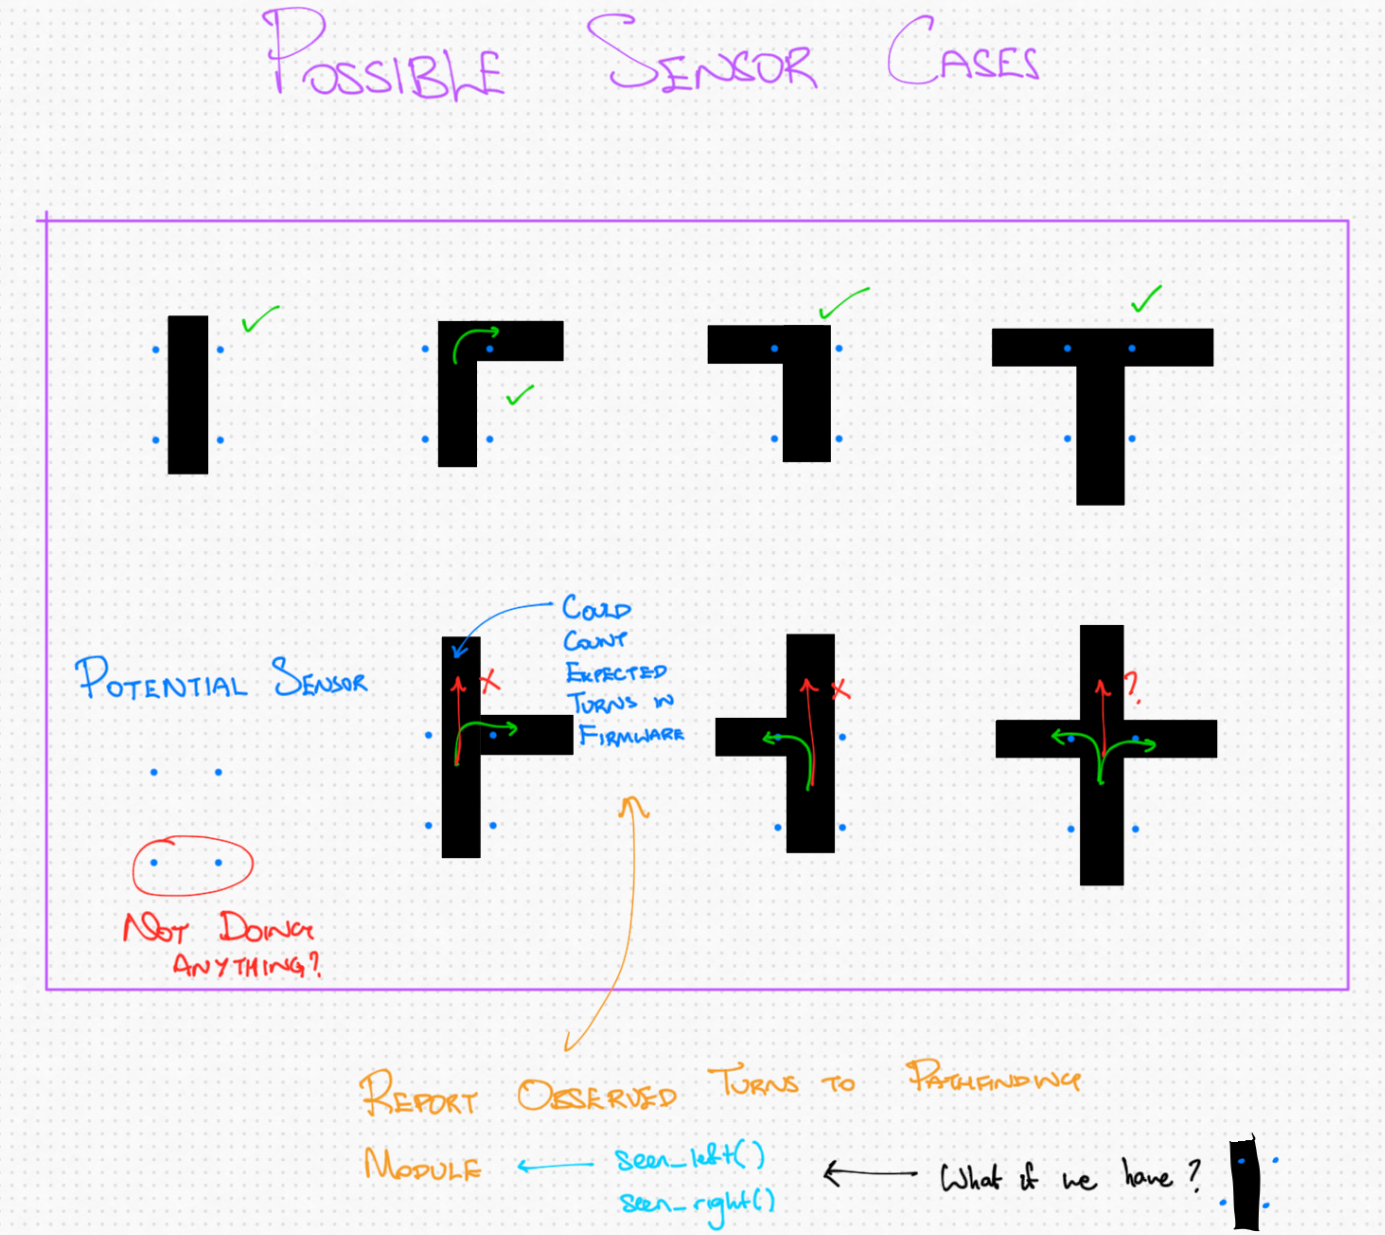
\includegraphics[width=0.4\textwidth]{constellation-basic-4-grid.png}}
% 	\caption{Basic 4-Grid sensor constellation}
% 	\label{fig:constellation-basic-4-grid}
% \end{figure}
% \begin{figure}[htbp]
% 	\centerline{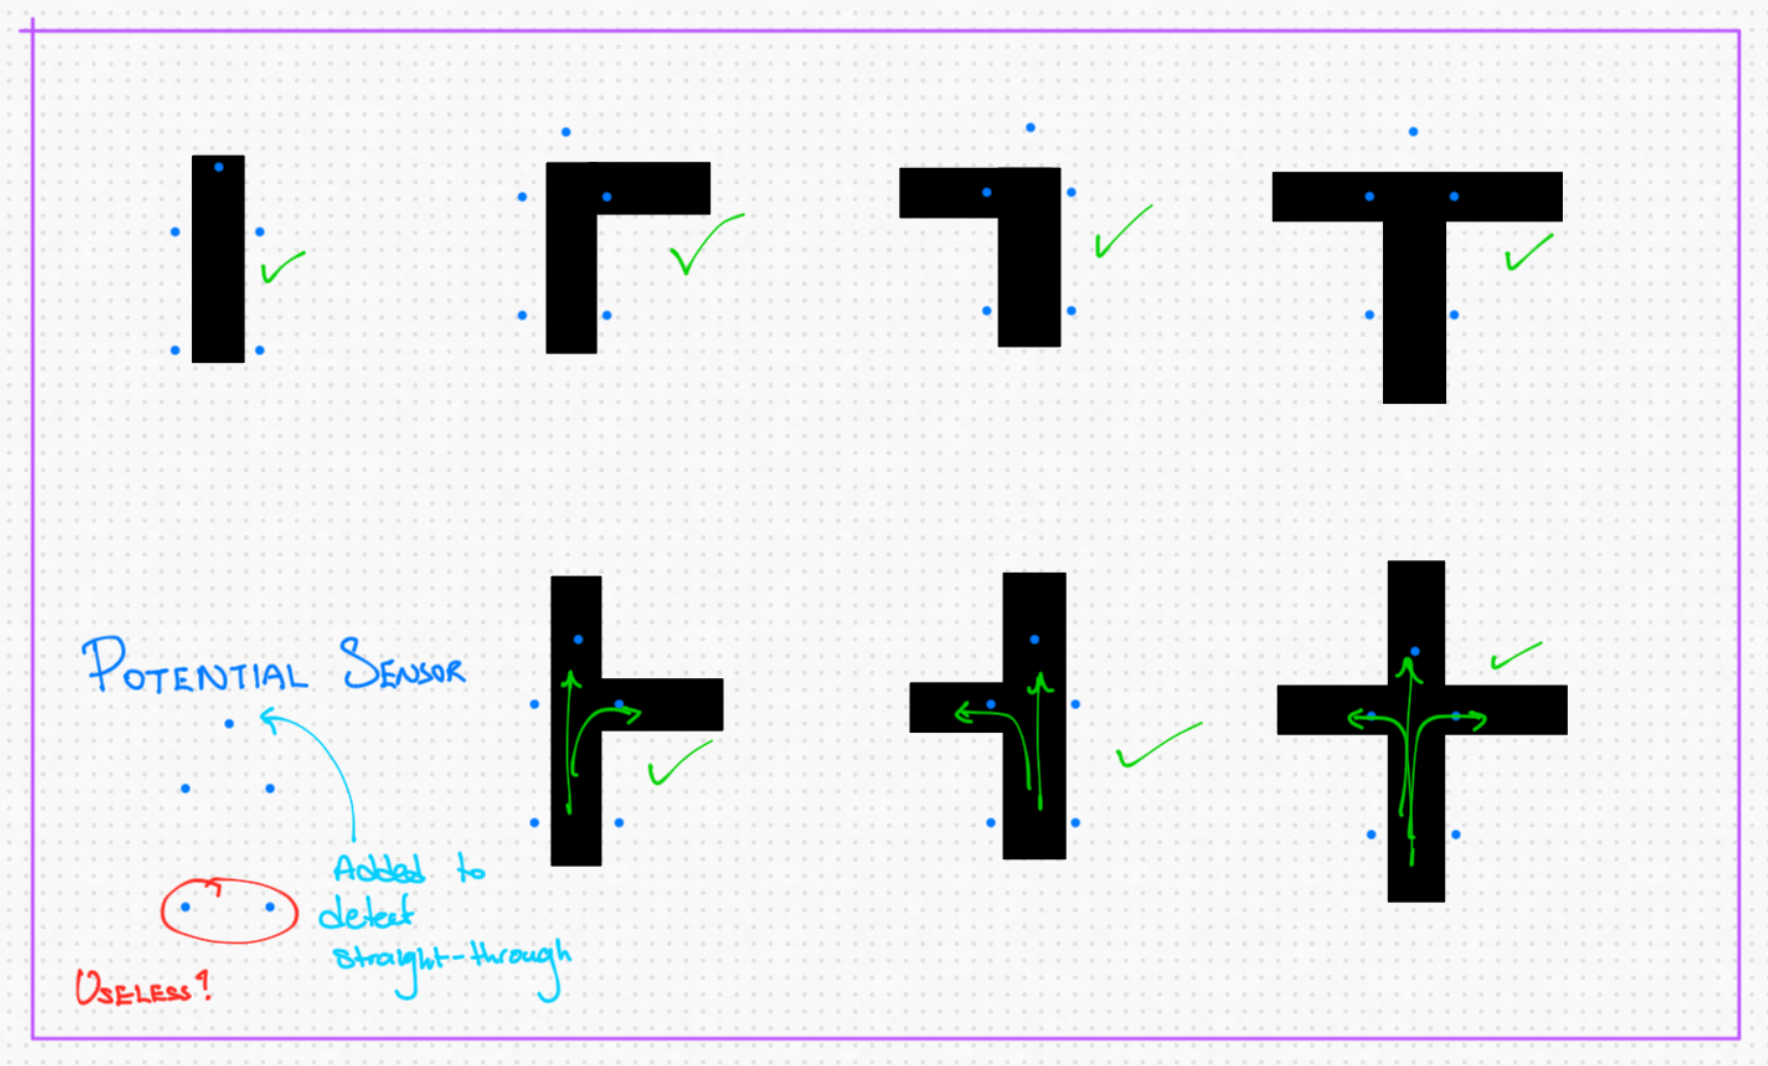
\includegraphics[width=0.4\textwidth]{constellation-basic-4-straight.png}}
% 	\caption{Basic 4-Grid with Straight-Ahead sensor constellation}
% 	\label{fig:constellation-basic-4-straight}
% \end{figure}
% \begin{figure}[htbp]
% 	\centerline{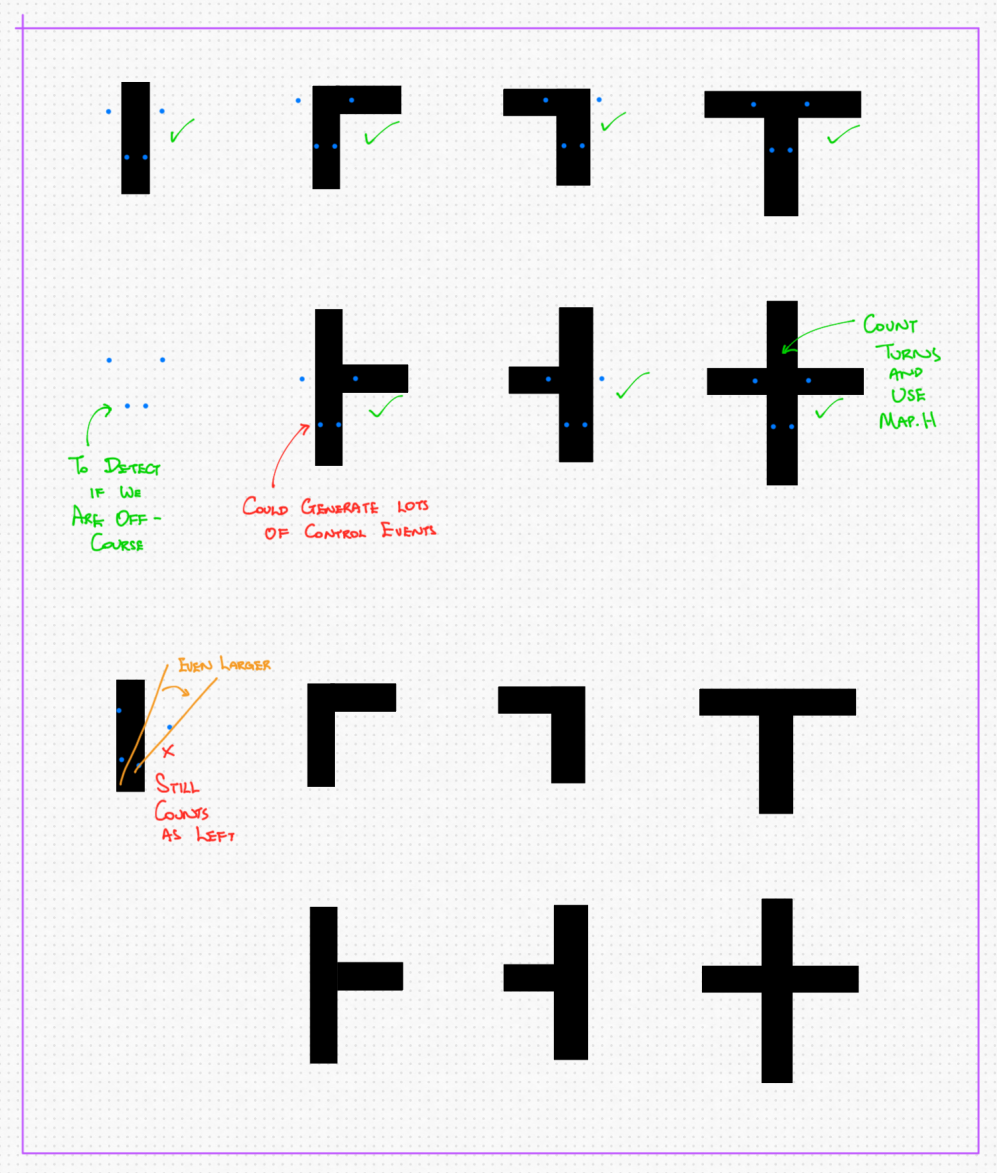
\includegraphics[width=0.4\textwidth]{constellation-4-skew-v1.png}}
% 	\caption{Modified 4-Grid with Skew Detection \texttt{v1} sensor constellation}
% 	\label{fig:constellation-4-skew-v1}
% \end{figure}
% \begin{figure}[htbp]
% 	\centerline{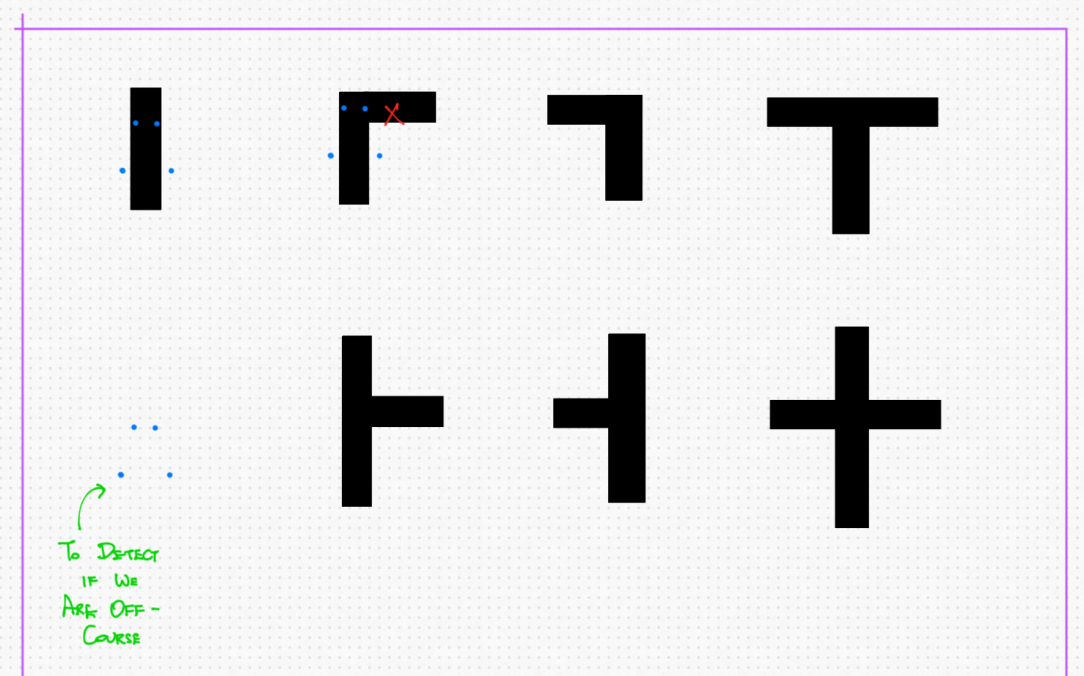
\includegraphics[width=0.4\textwidth]{constellation-4-skew-v2.png}}
% 	\caption{Modified 4-Grid with Skew Detection \texttt{v2} sensor constellation}
% 	\label{fig:constellation-4-skew-v2}
% \end{figure}
% \begin{figure}[htbp]
% 	\centerline{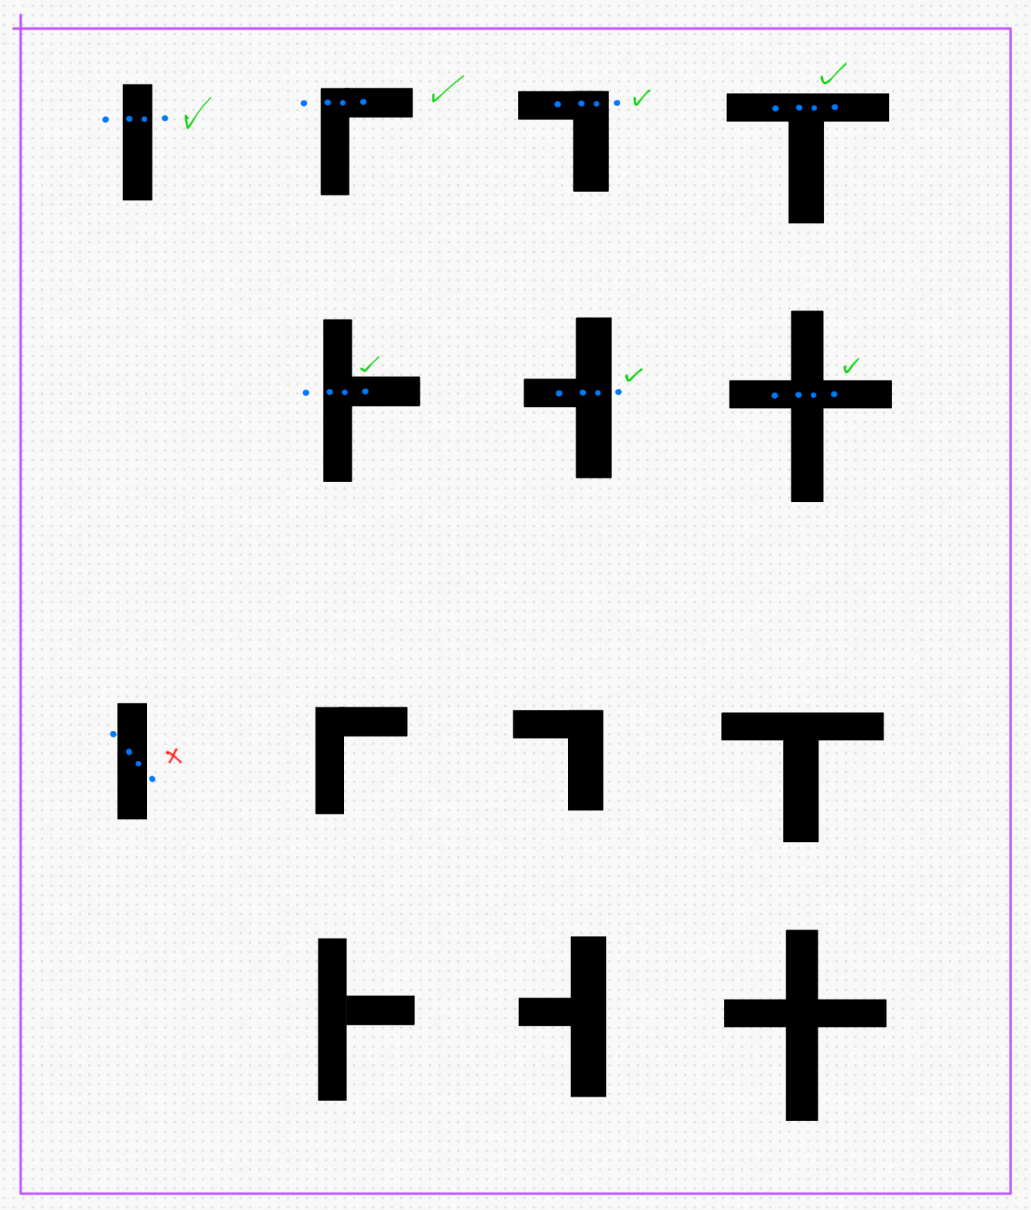
\includegraphics[width=0.4\textwidth]{constellation-4-line.png}}
% 	\caption{4-Line sensor constellation}
% 	\label{fig:constellation-4-line}
% \end{figure}
% \begin{figure}[htbp]
% 	\centerline{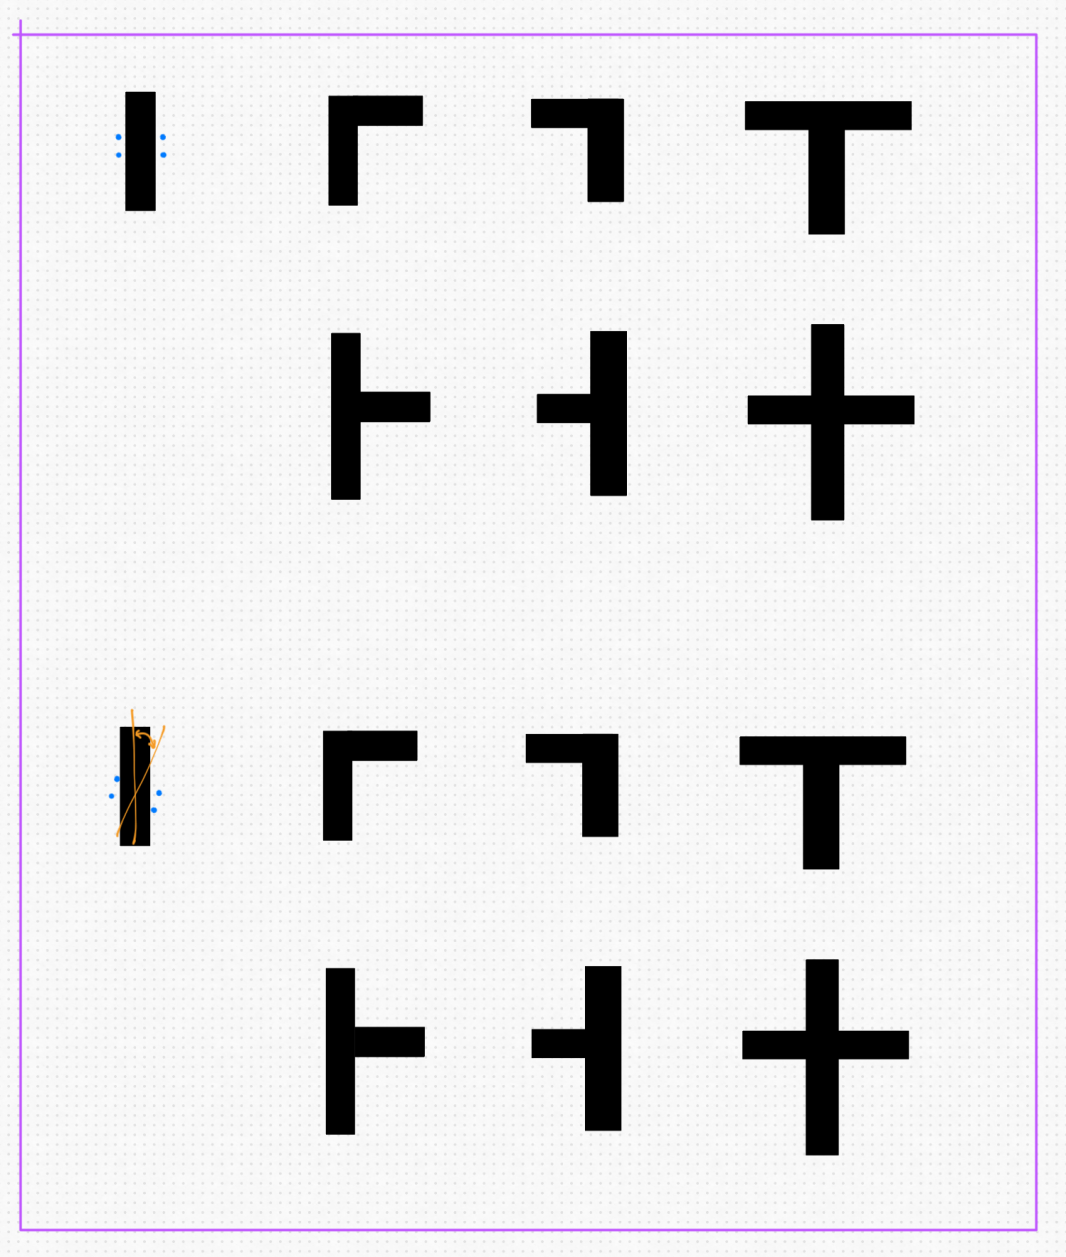
\includegraphics[width=0.4\textwidth]{constellation-4-skew-v3.png}}
% 	\caption{Modified 4-Grid with Skew Detection \texttt{v3} sensor constellation}
% 	\label{fig:constellation-4-skew-v3}
% \end{figure}
% \begin{figure}[htbp]
% 	\centerline{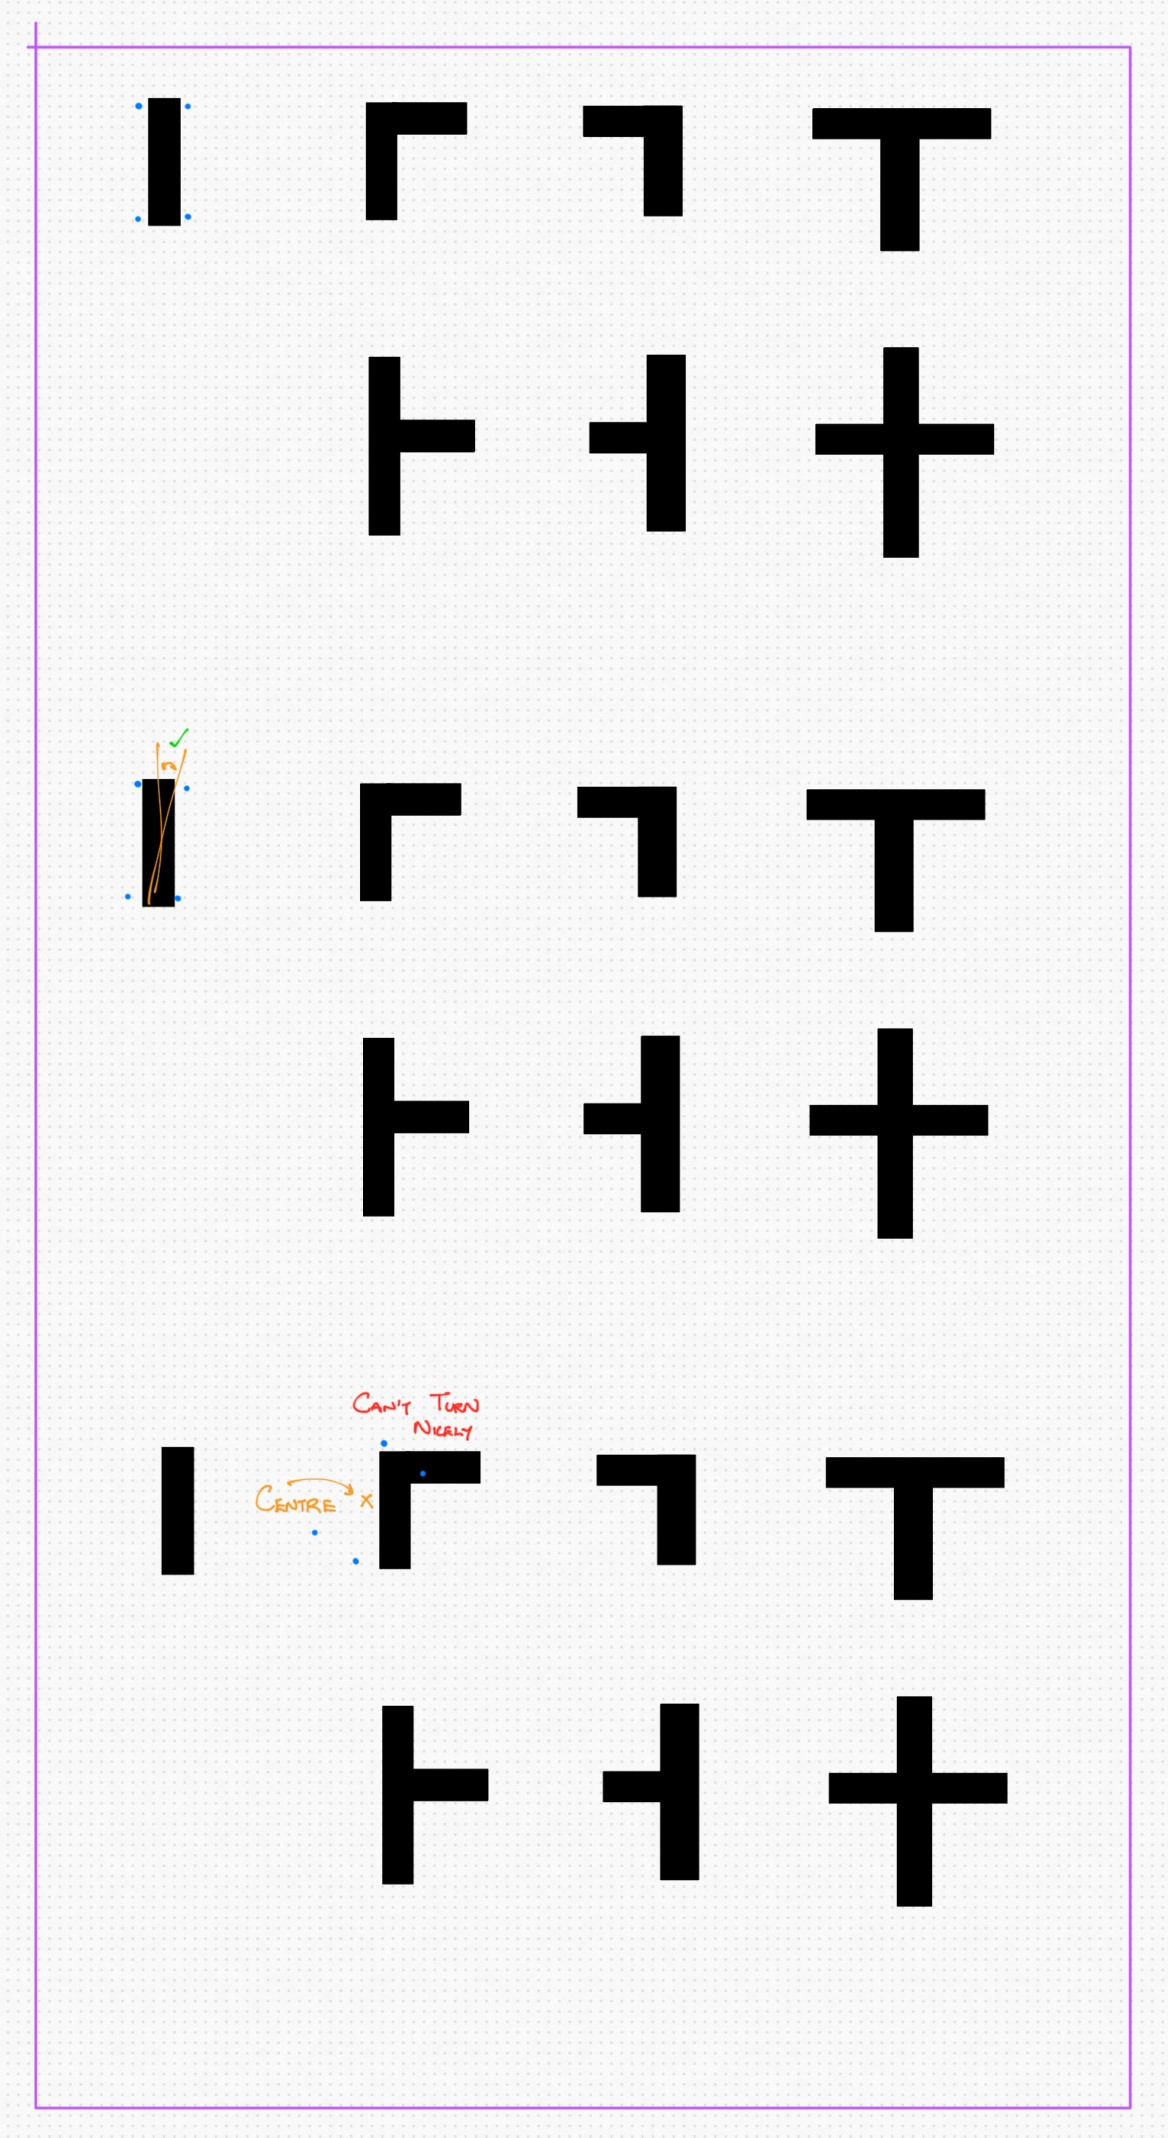
\includegraphics[width=0.4\textwidth]{constellation-4-skew-v4.png}}
% 	\caption{Modified 4-Grid with Skew Detection \texttt{v4} sensor constellation}
% 	\label{fig:constellation-4-skew-v4}
% \end{figure}
% \begin{figure}[htbp]
% 	\centerline{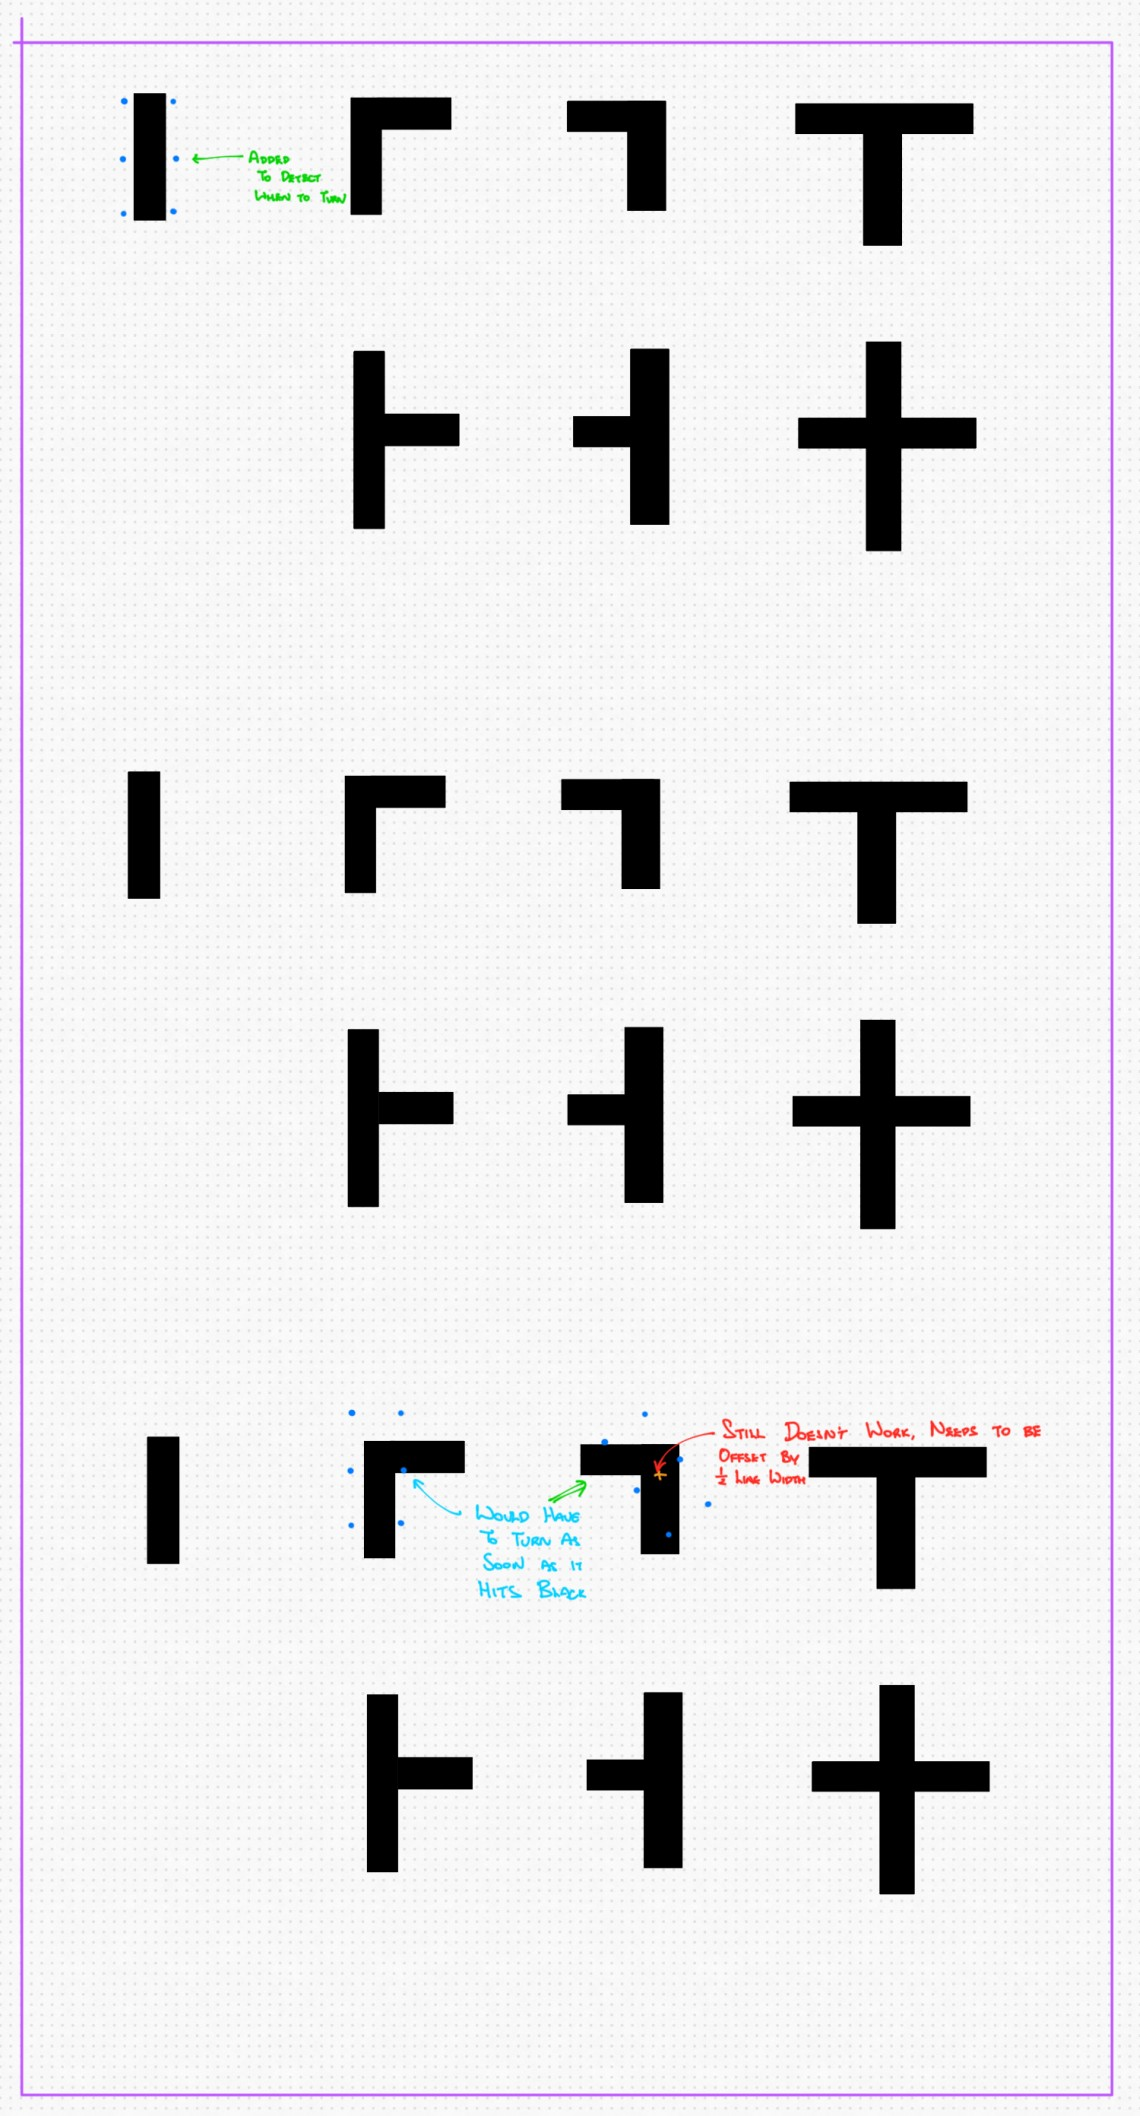
\includegraphics[width=0.4\textwidth]{constellation-6-grid.png}}
% 	\caption{6-Grid sensor constellation}
% 	\label{fig:constellation-6-grid}
% \end{figure}
% \begin{figure}[htbp]
% 	\centerline{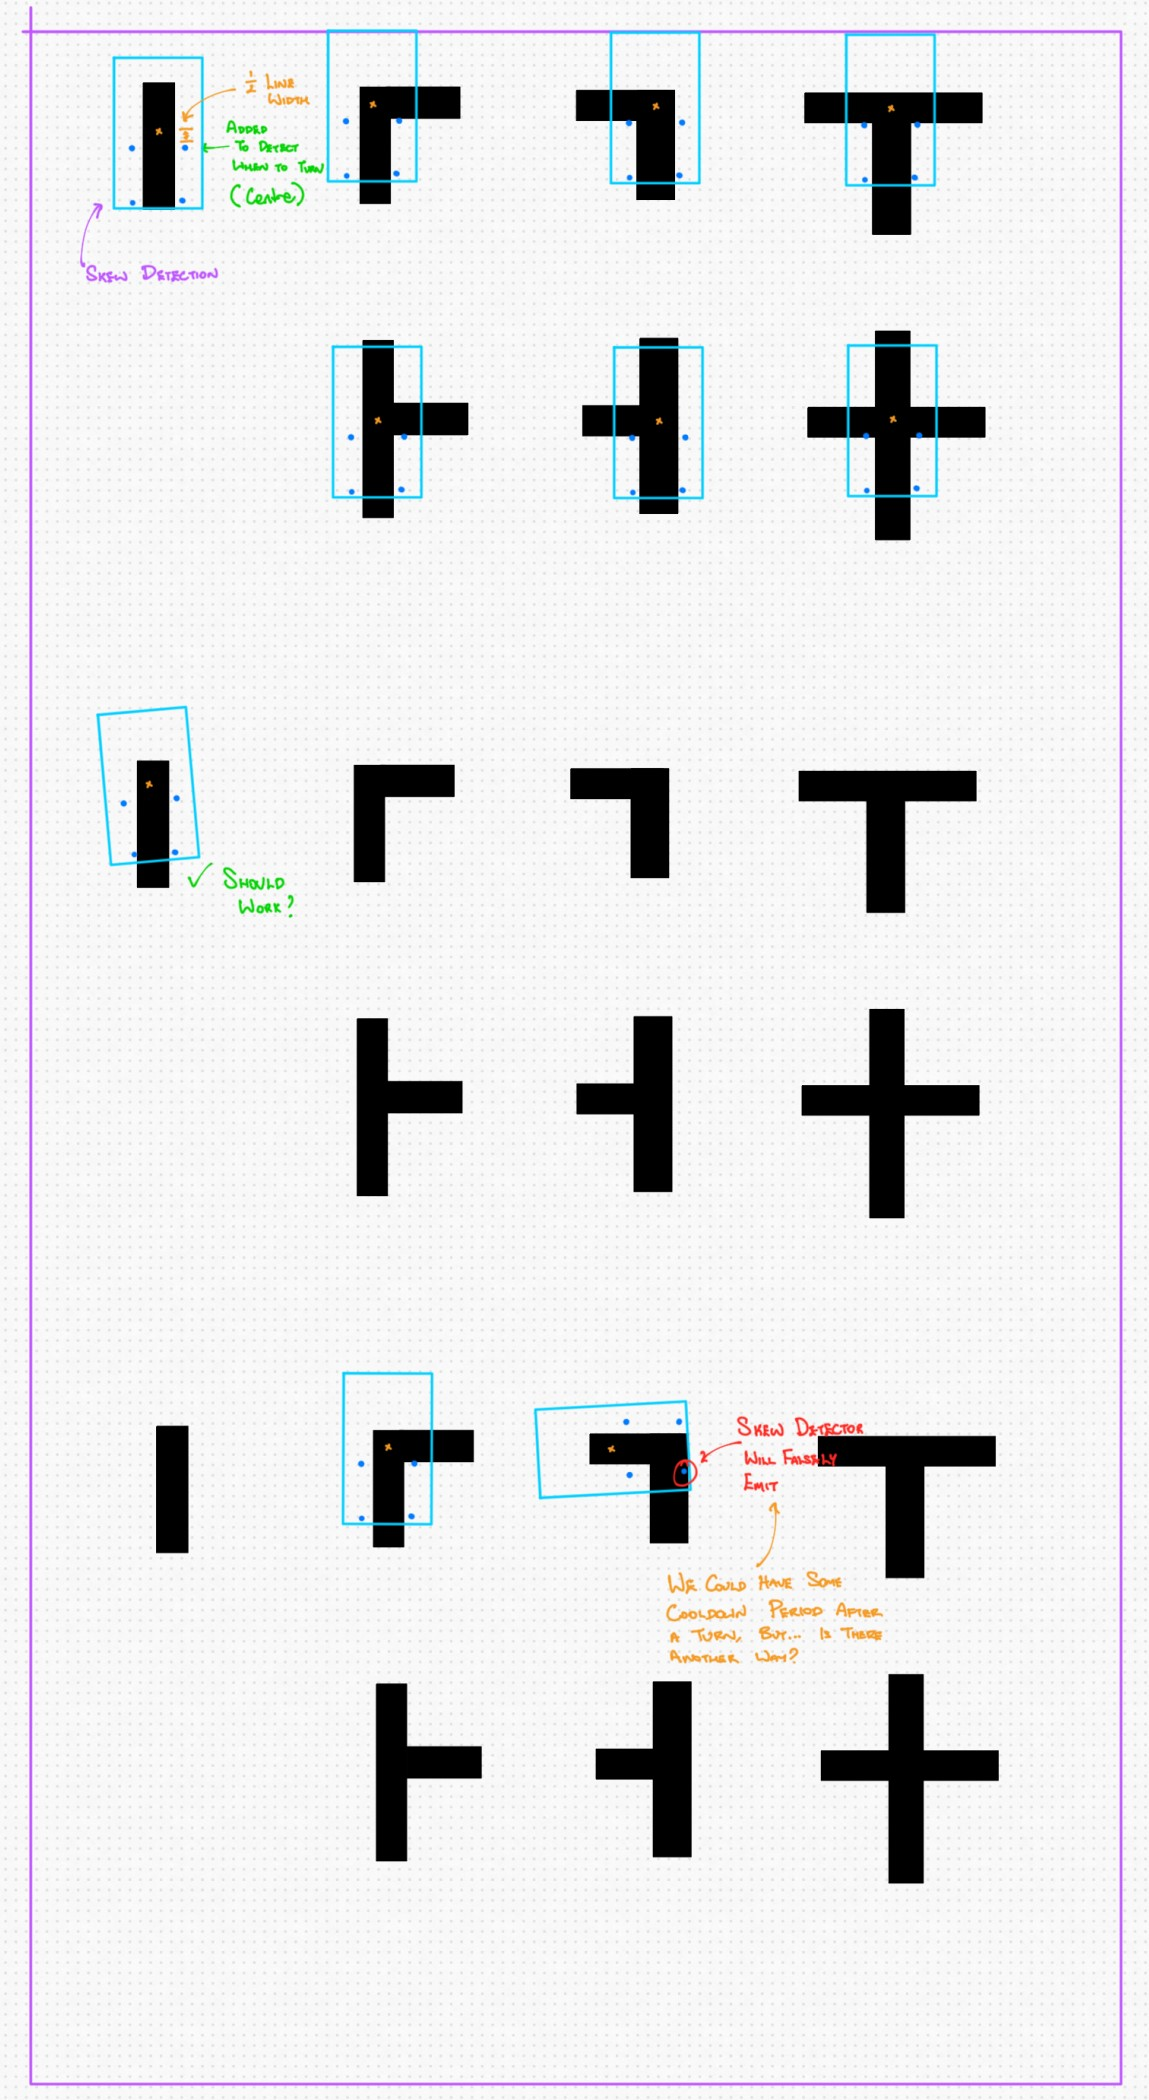
\includegraphics[width=0.4\textwidth]{constellation-4-offset.png}}
% 	\caption{Modified 4-Grid with Offset Middle Sensors sensor constellation}
% 	\label{fig:constellation-4-offset}
% \end{figure}
% \begin{figure}[htbp]
% 	\centerline{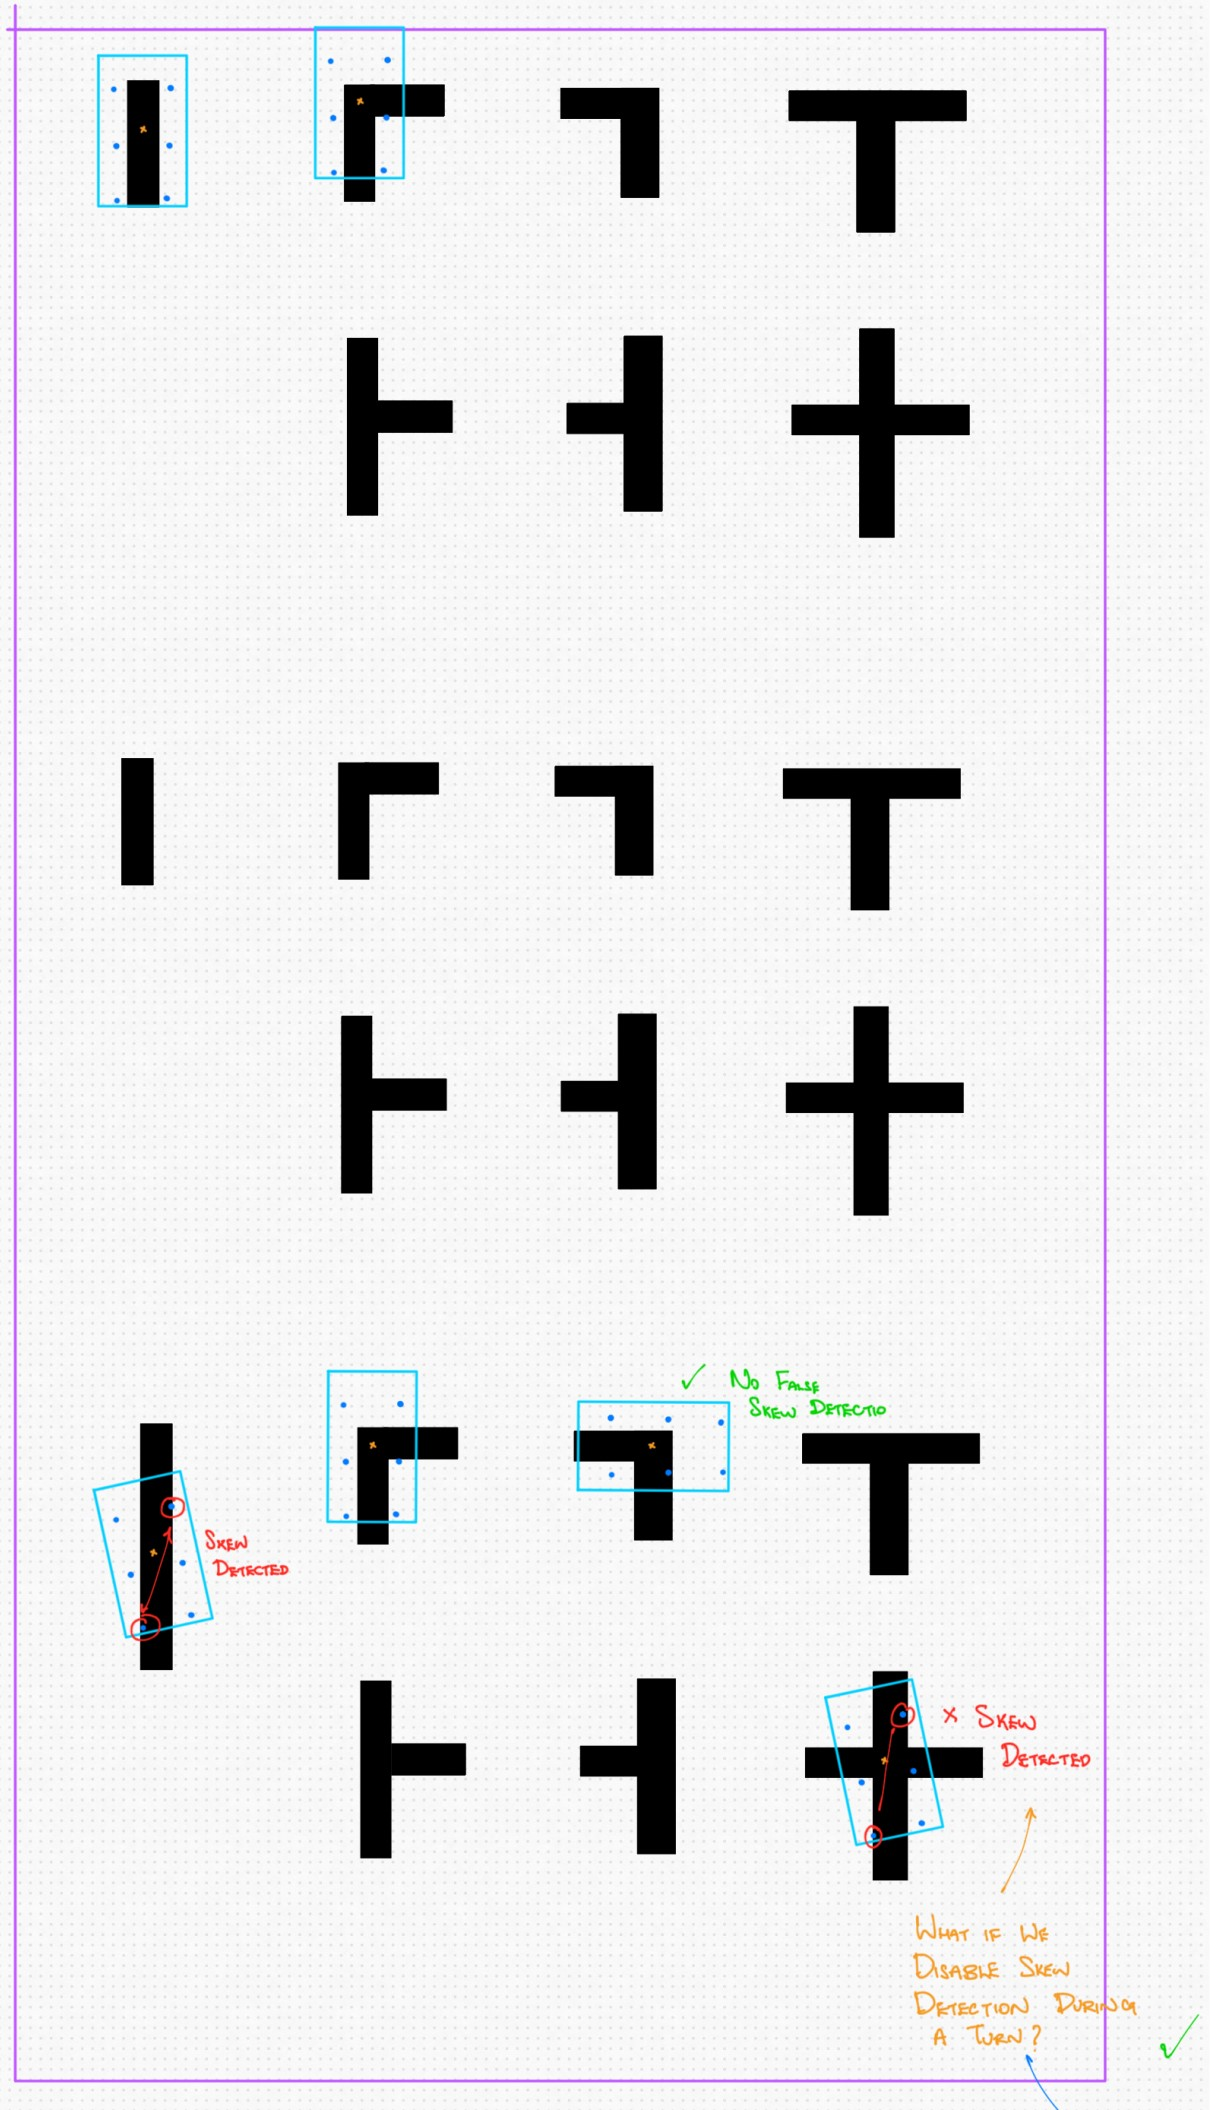
\includegraphics[width=0.4\textwidth]{constellation-6-offset.png}}
% 	\caption{Modified 6-Grid with Offset Middle Sensors sensor constellation}
% 	\label{fig:constellation-6-offset}
% \end{figure}
% \begin{figure}[htbp]
% 	\centerline{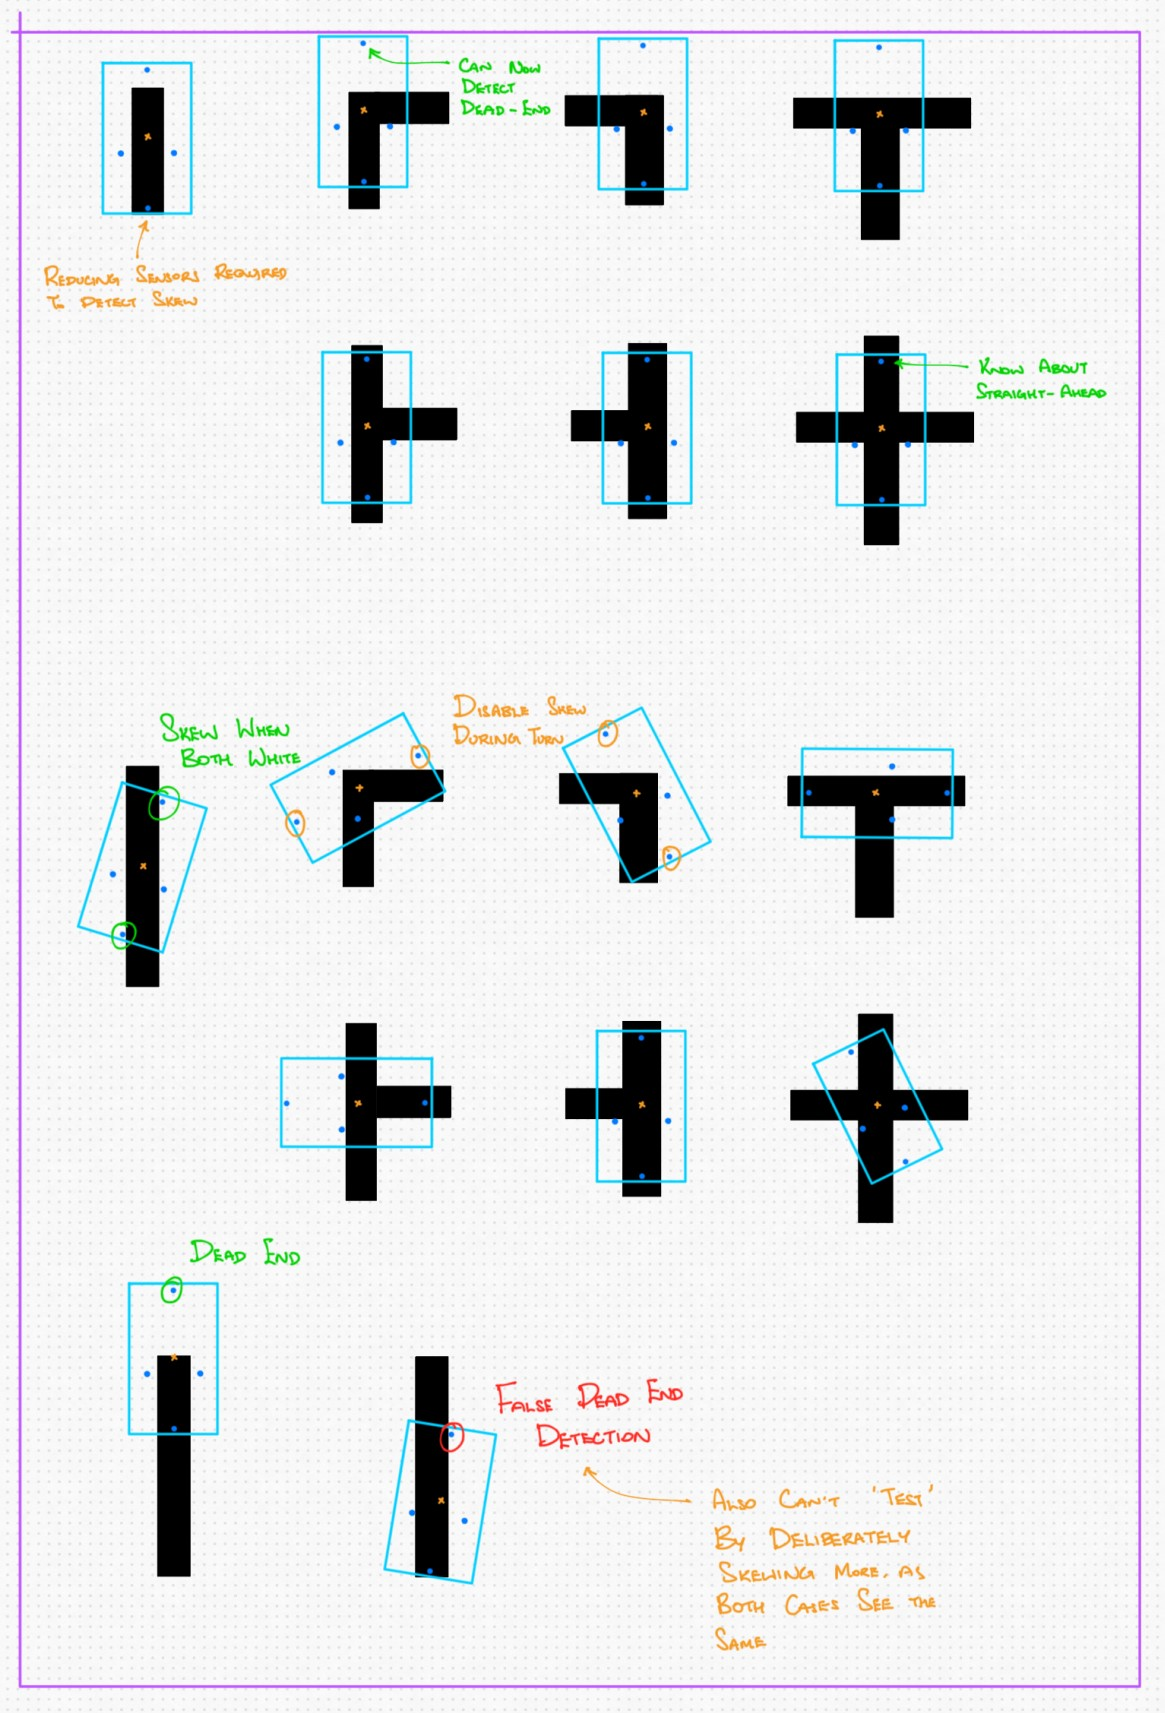
\includegraphics[width=0.4\textwidth]{constellation-diamond.png}}
% 	\caption{Diamond sensor constellation}
% 	\label{fig:constellation-diamond}
% \end{figure}
% \begin{figure}[htbp]
% 	\centerline{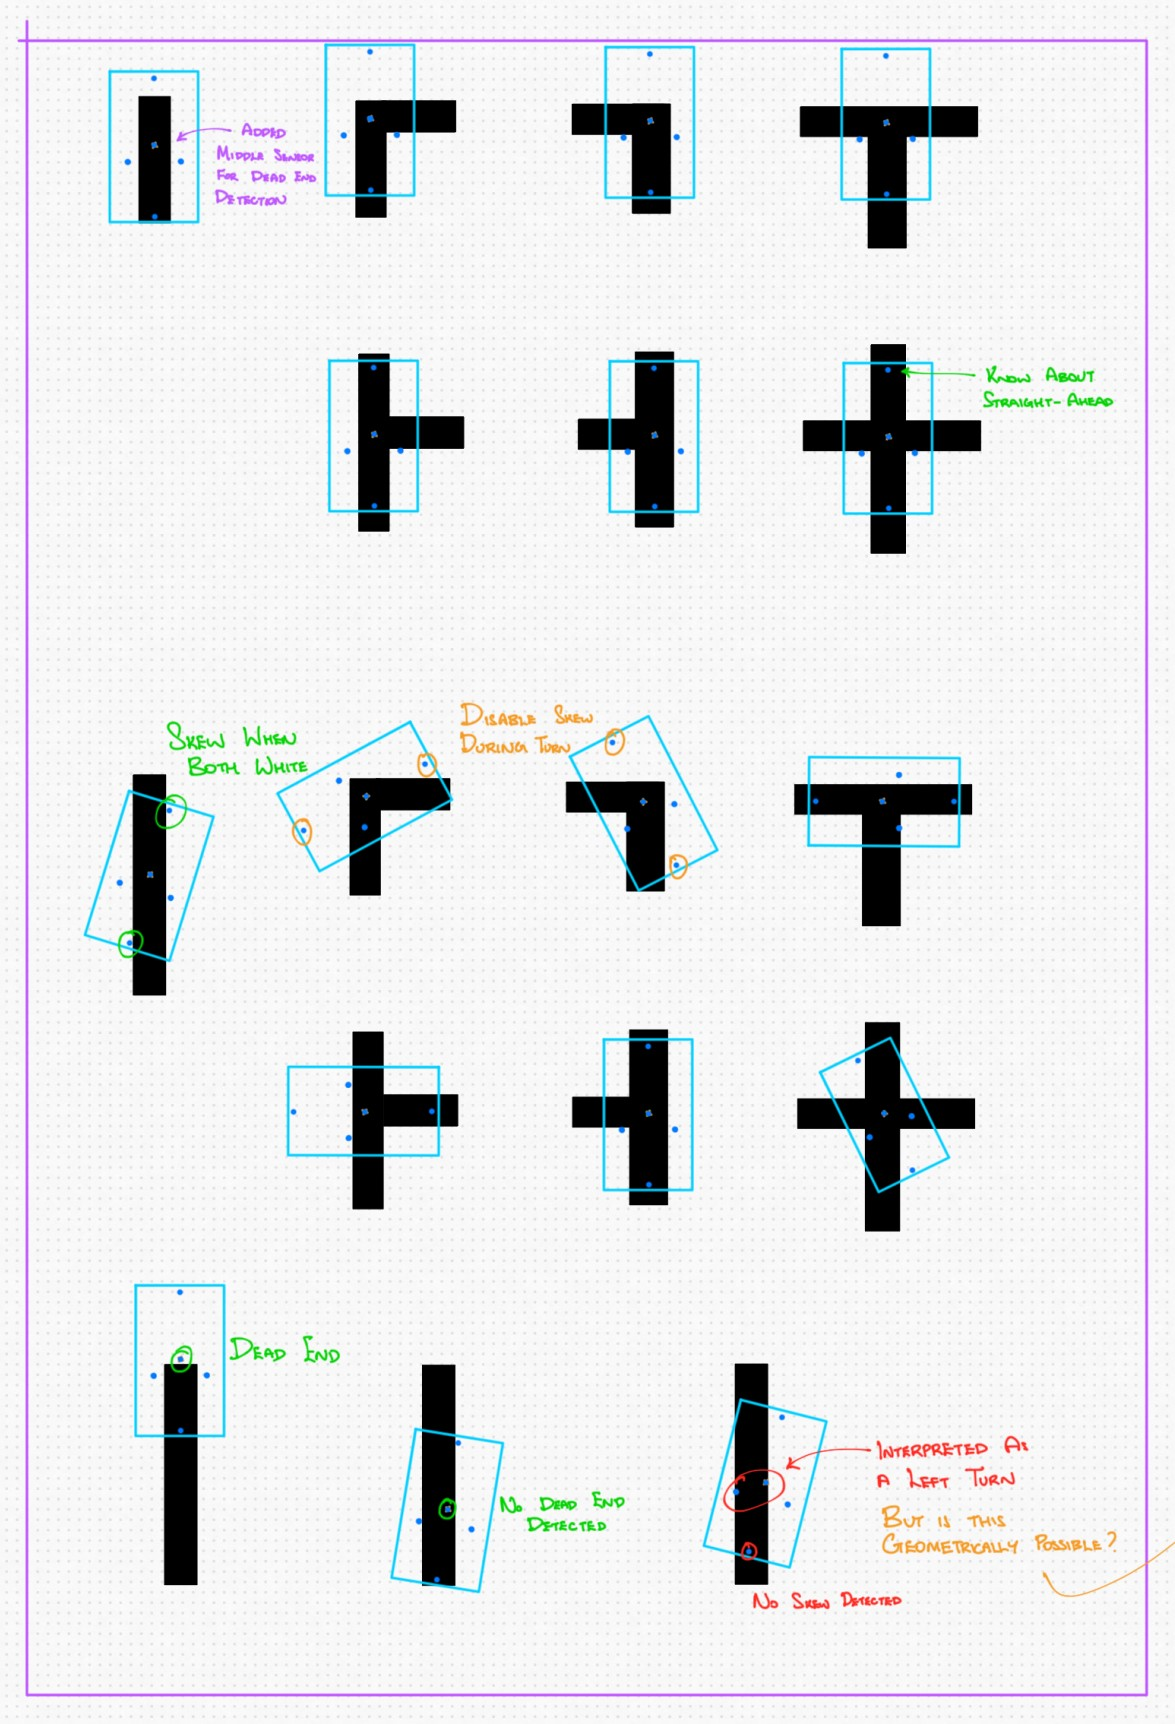
\includegraphics[width=0.4\textwidth]{constellation-diamond-middle.png}}
% 	\caption{Modified Diamond with Middle Sensor sensor constellation}
% 	\label{fig:constellation-diamond-middle}
% \end{figure}
% \begin{figure}[htbp]
% 	\centerline{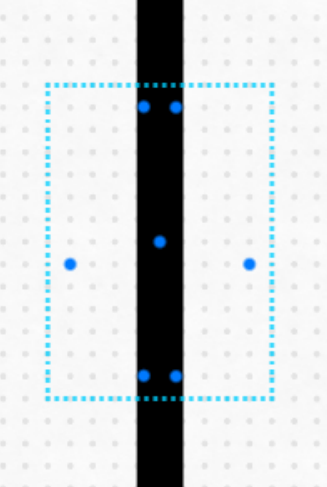
\includegraphics[width=0.2\textwidth]{constellation-hexagon-middle.png}}
% 	\caption{Hexagon with Middle Sensor sensor constellation}
% 	\label{fig:constellation-hexagon-middle}
% \end{figure}

% \begin{figure}[htbp]
% 	\centerline{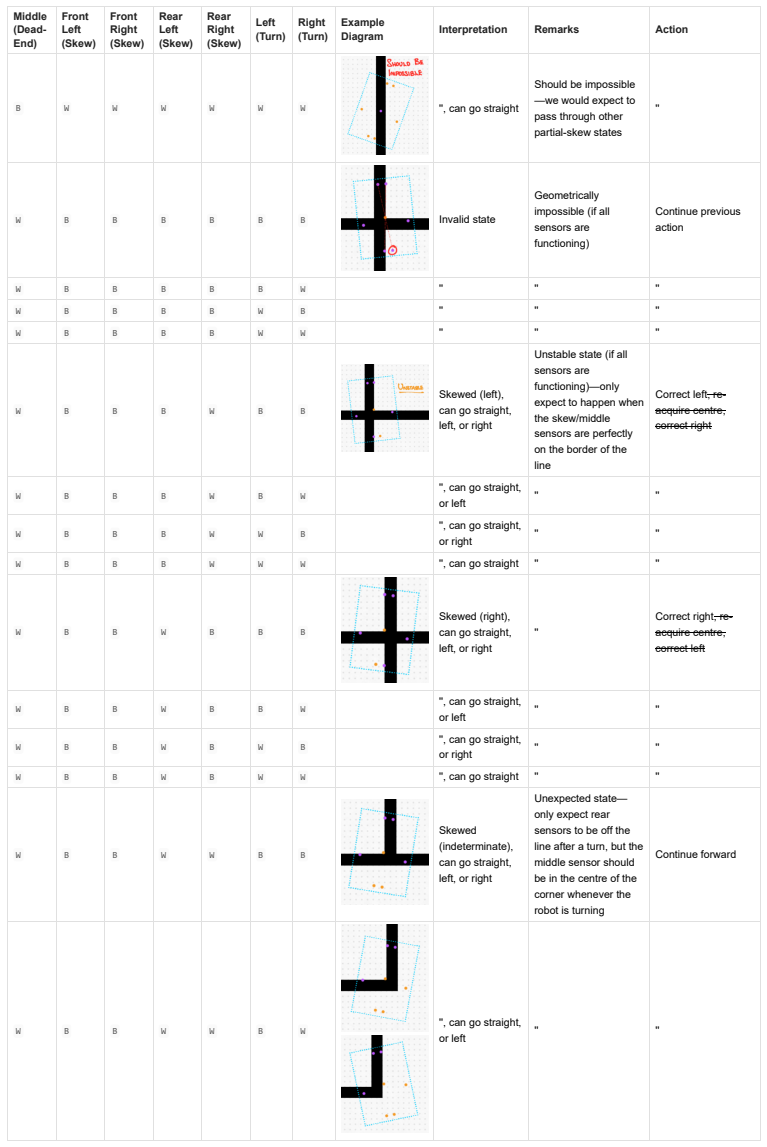
\includegraphics[width=0.5\textwidth]{sensor-table.png}}
% 	\caption{Selection of rows from sensor constellation truth table}
% 	\label{fig:sensor-table}
% \end{figure}
% \begin{figure}[htbp]
% 	\centerline{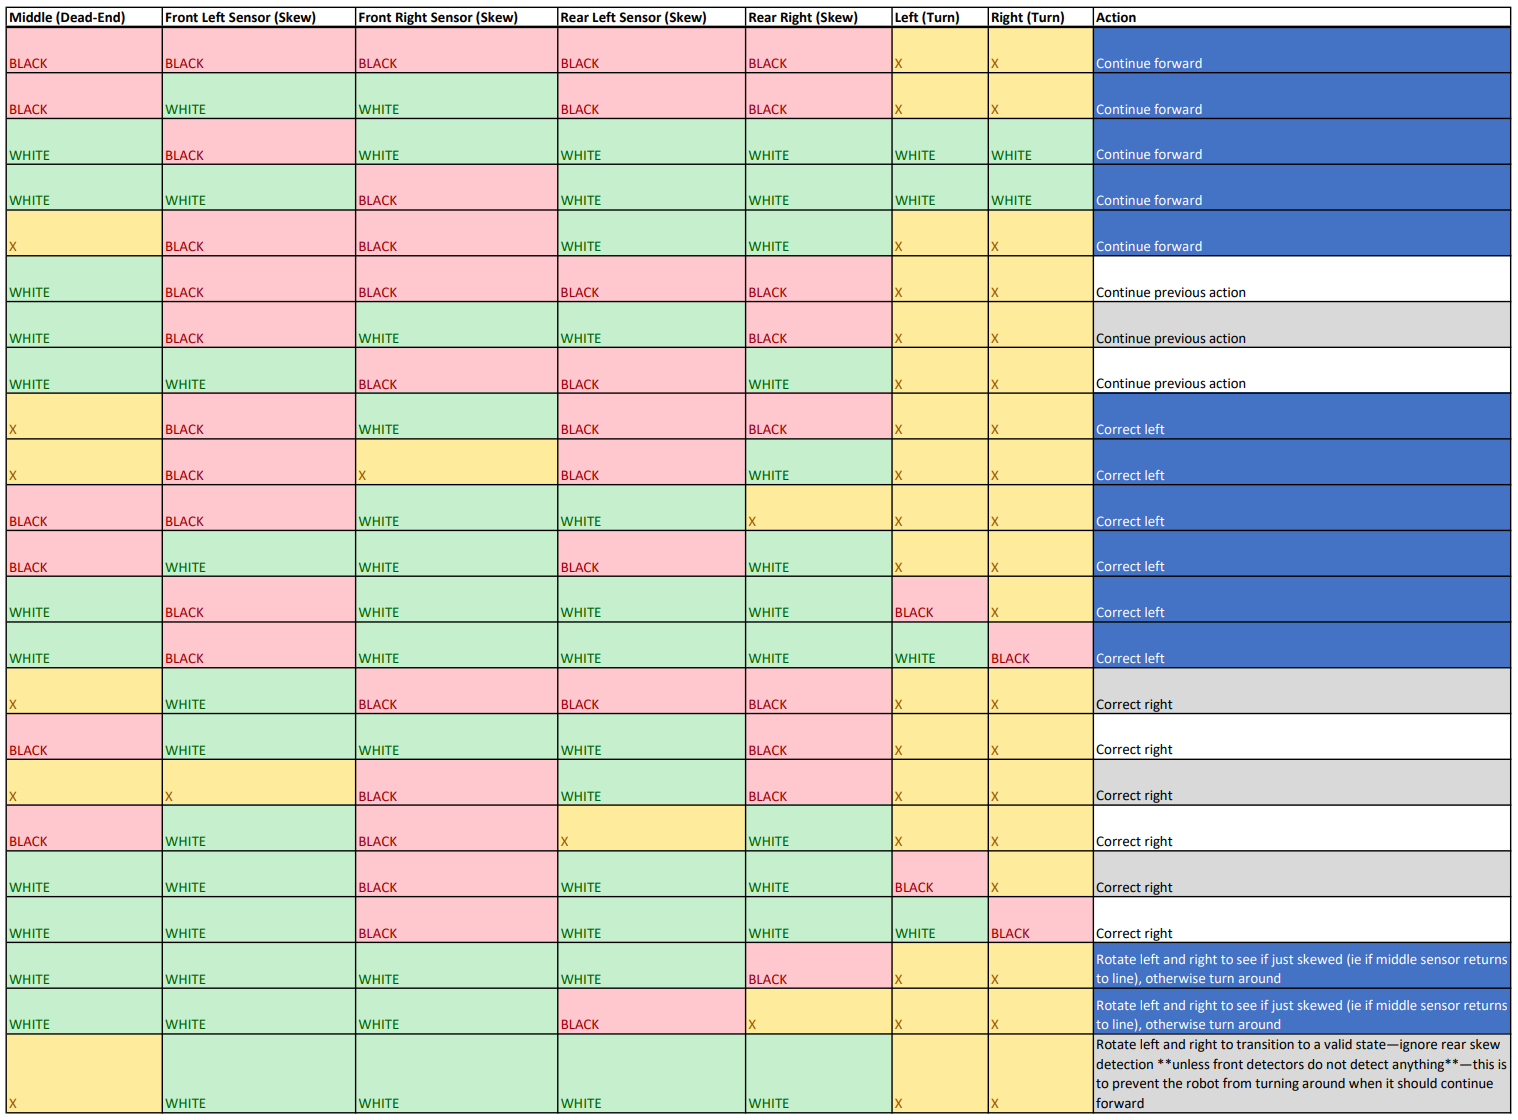
\includegraphics[width=0.5\textwidth]{sensor-table-reduced.png}}
% 	\caption{Reduced sensor constellation truth table}
% 	\label{fig:sensor-table-reduced}
% \end{figure}

% \begin{figure}[htbp]
% 	\centerline{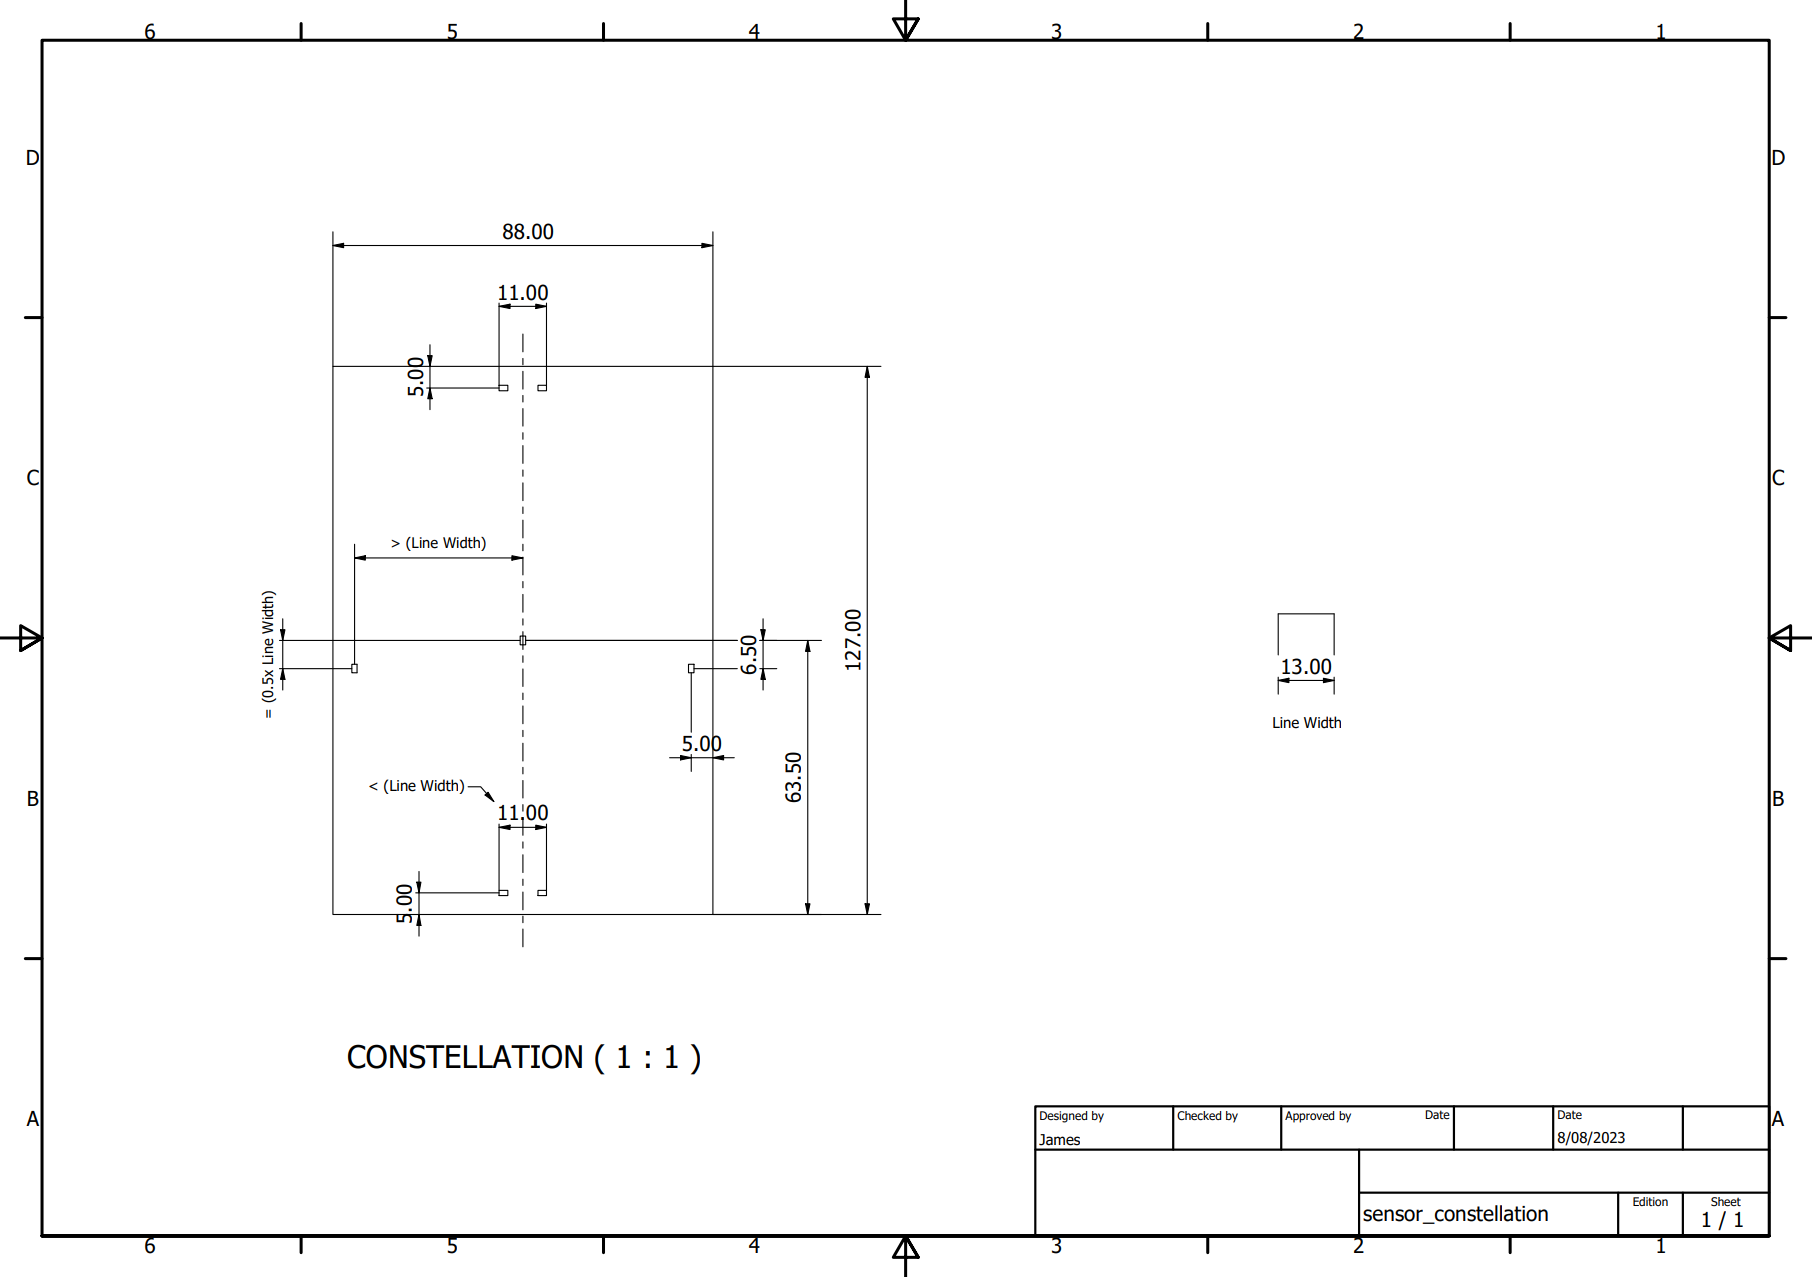
\includegraphics[width=0.5\textwidth]{constellation-cad.png}}
% 	\caption{Dimensioned CAD drawing for final constellation design}
% 	\label{fig:constellation-cad}
% \end{figure}

% \subsection{Pathfinding Implementation}

% \begin{figure}[htbp]
% 	\centerline{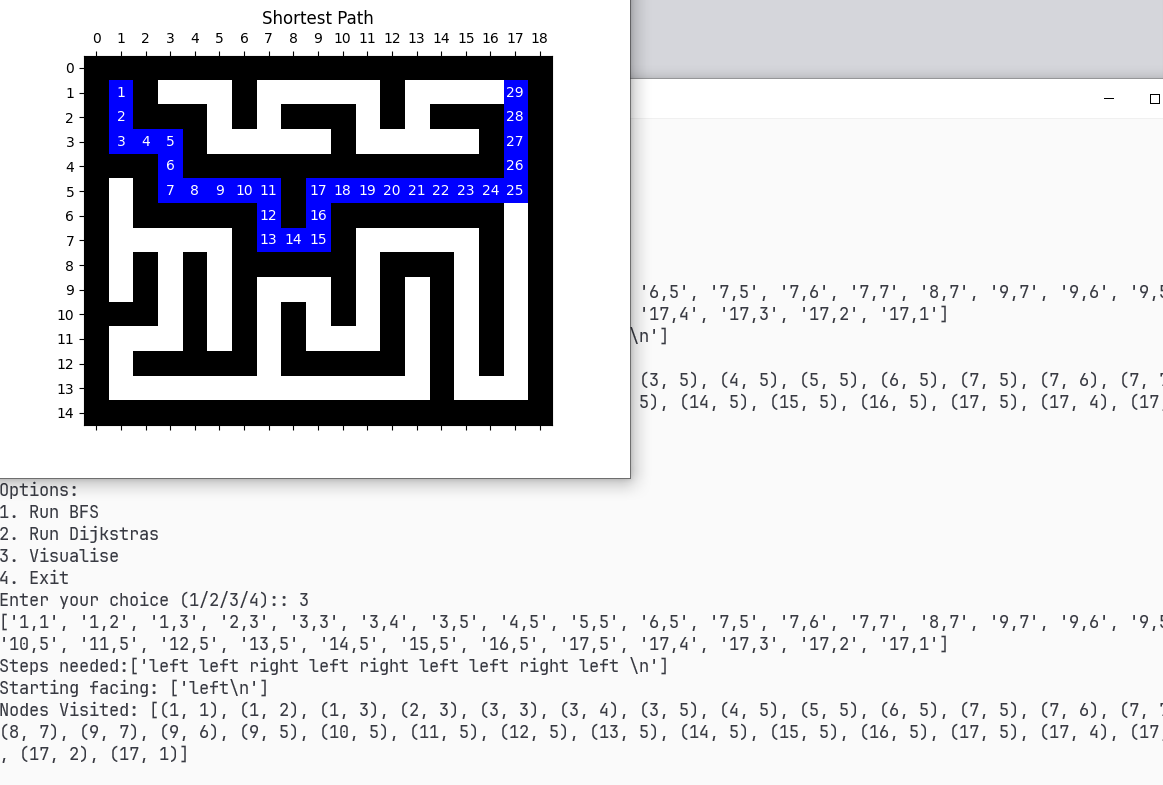
\includegraphics[width=0.5\textwidth]{pathfinding-visualisation.png}}
% 	\caption{Pathfinding visualisation tool created with \texttt{Matplotlib}}
% 	\label{fig:pathfinding-visualisation}
% \end{figure}
% \begin{figure}[htbp]
% 	\centerline{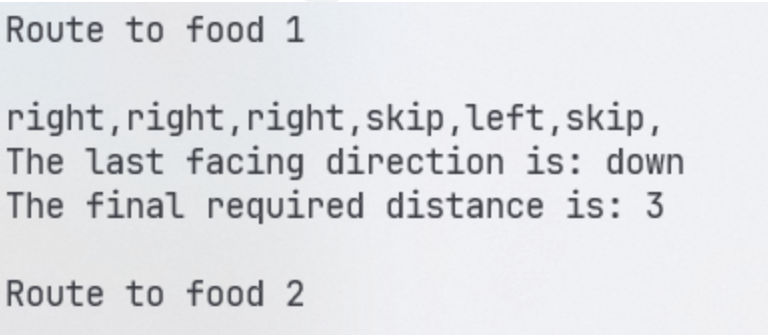
\includegraphics[width=0.5\textwidth]{pathfinding-instructions.png}}
% 	\caption{Debugging output of the generated instructions}
% 	\label{fig:pathfinding-instructions}
% \end{figure}

% \subsection{Movement Module}

% \begin{figure}[htbp]
% 	\centerline{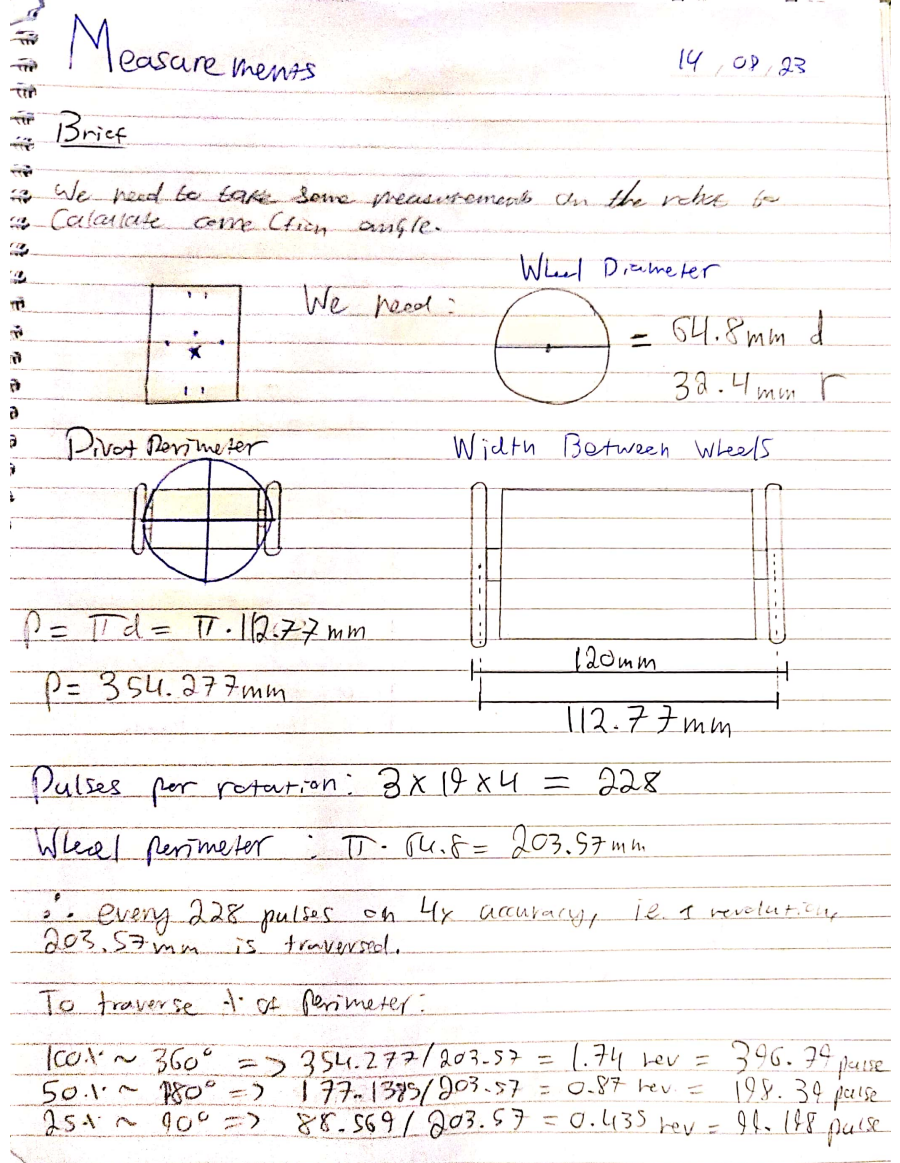
\includegraphics[width=0.5\textwidth]{physical-measurements.png}}
% 	\caption{Measurements of the robot's physical dimensions}
% 	\label{fig:physical-dimensions}
% \end{figure}

% \subsection{Sensor Processing Module}

% \begin{figure}[htbp]
% 	\centerline{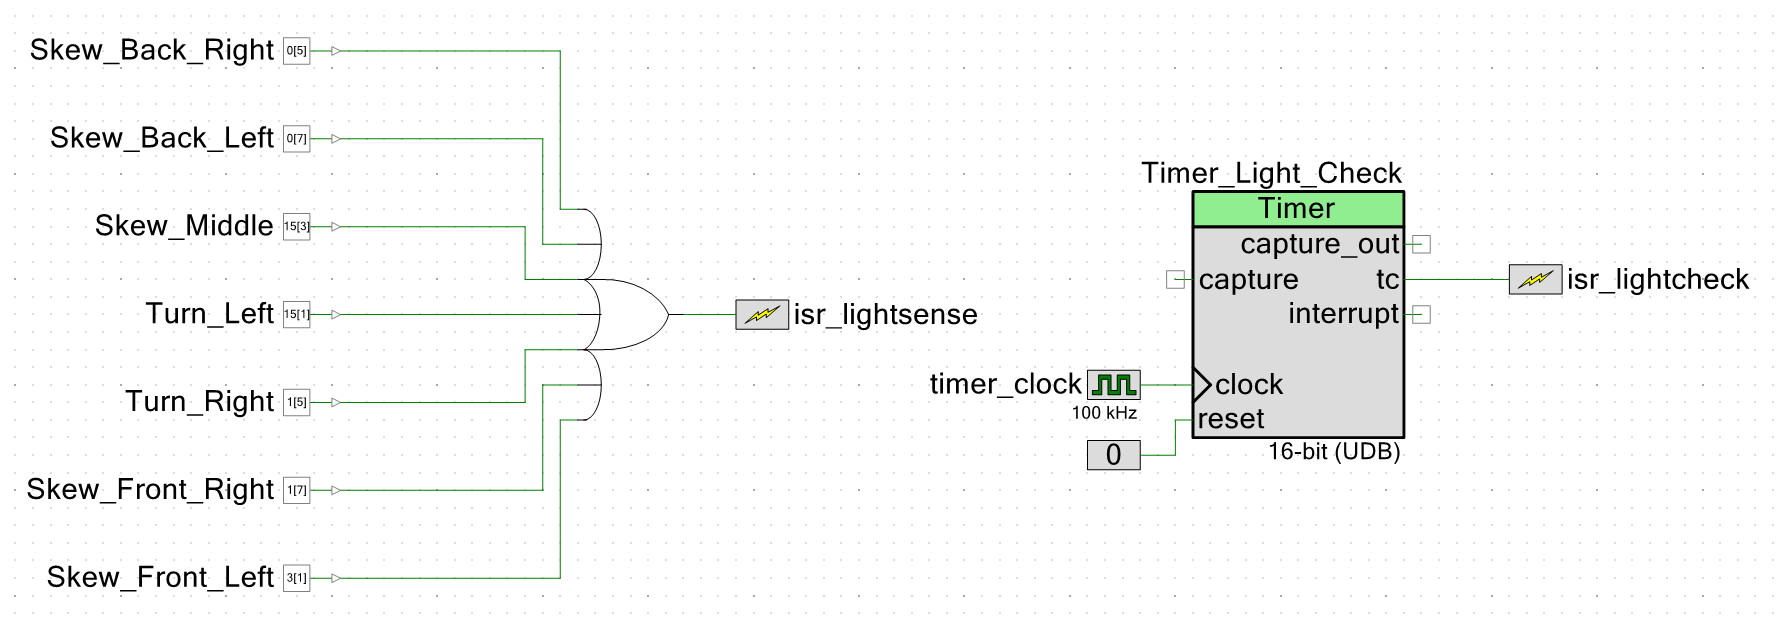
\includegraphics[width=0.5\textwidth]{sensor-psoc.png}}
% 	\caption{Screenshot of PSoC components used in sensor processing}
% 	\label{fig:sensor-psoc}
% \end{figure}

% \begin{figure}[htbp]
% 	\centerline{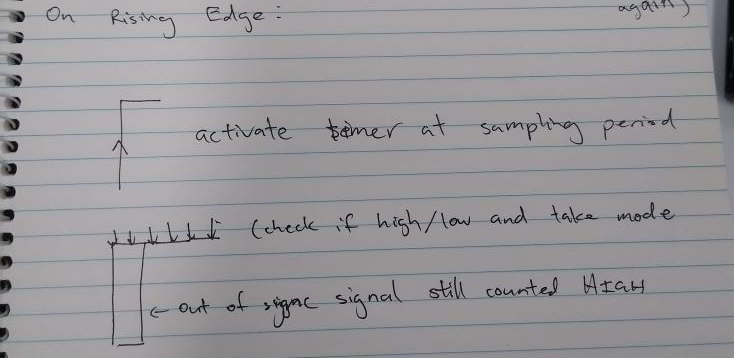
\includegraphics[width=0.5\textwidth]{sensor-sampling.png}}
% 	\caption{Explanation of sensor sampling process}
% 	\label{fig:sensor-sampling}
% \end{figure}
% \begin{figure}[htbp]
% 	\centerline{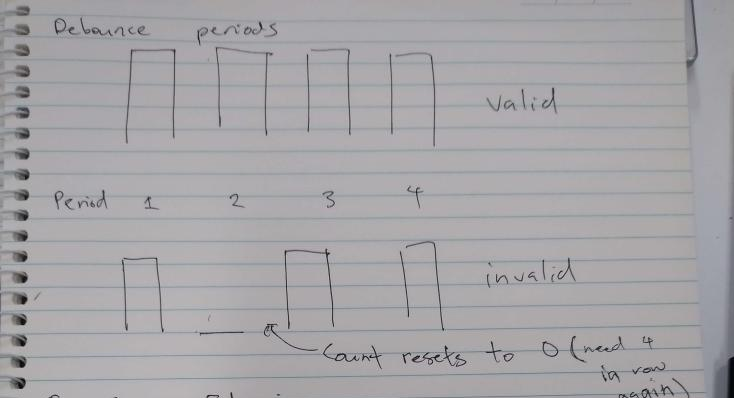
\includegraphics[width=0.5\textwidth]{sensor-debouncing.png}}
% 	\caption{Explanation of sensor debouncing process}
% 	\label{fig:sensor-debouncing}
% \end{figure}

% \subsection{Pathfinding Module}

% \begin{figure}[htbp]
% 	\centerline{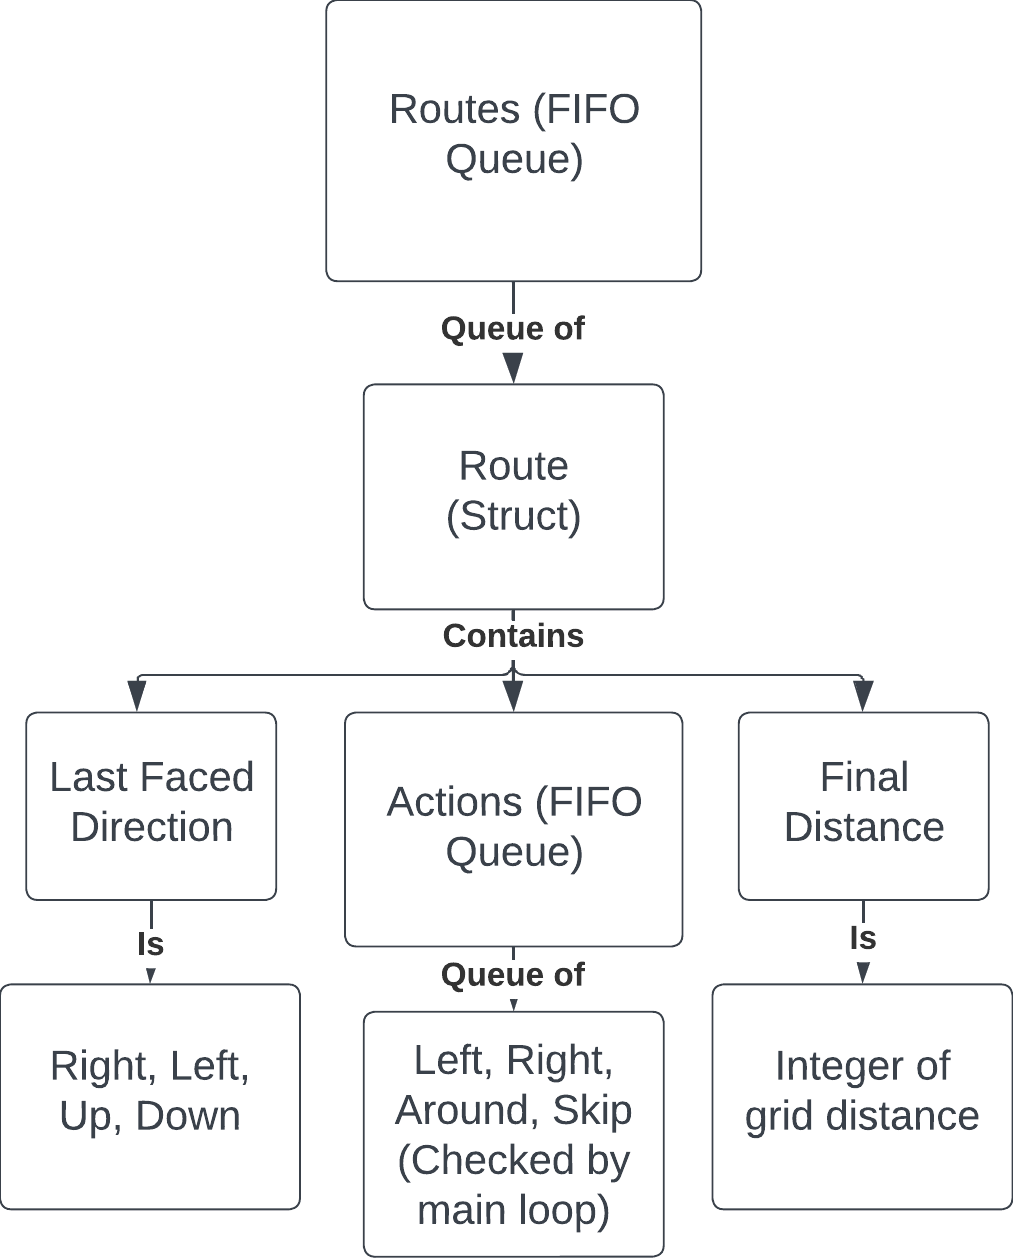
\includegraphics[width=0.3\textwidth]{pathfinding-route-struct.png}}
% 	\caption{Our route data structure}
% 	\label{fig:pathfinding-route-struct}
% \end{figure}

% \subsection{Integration}

% \begin{figure}[htbp]
% 	\centerline{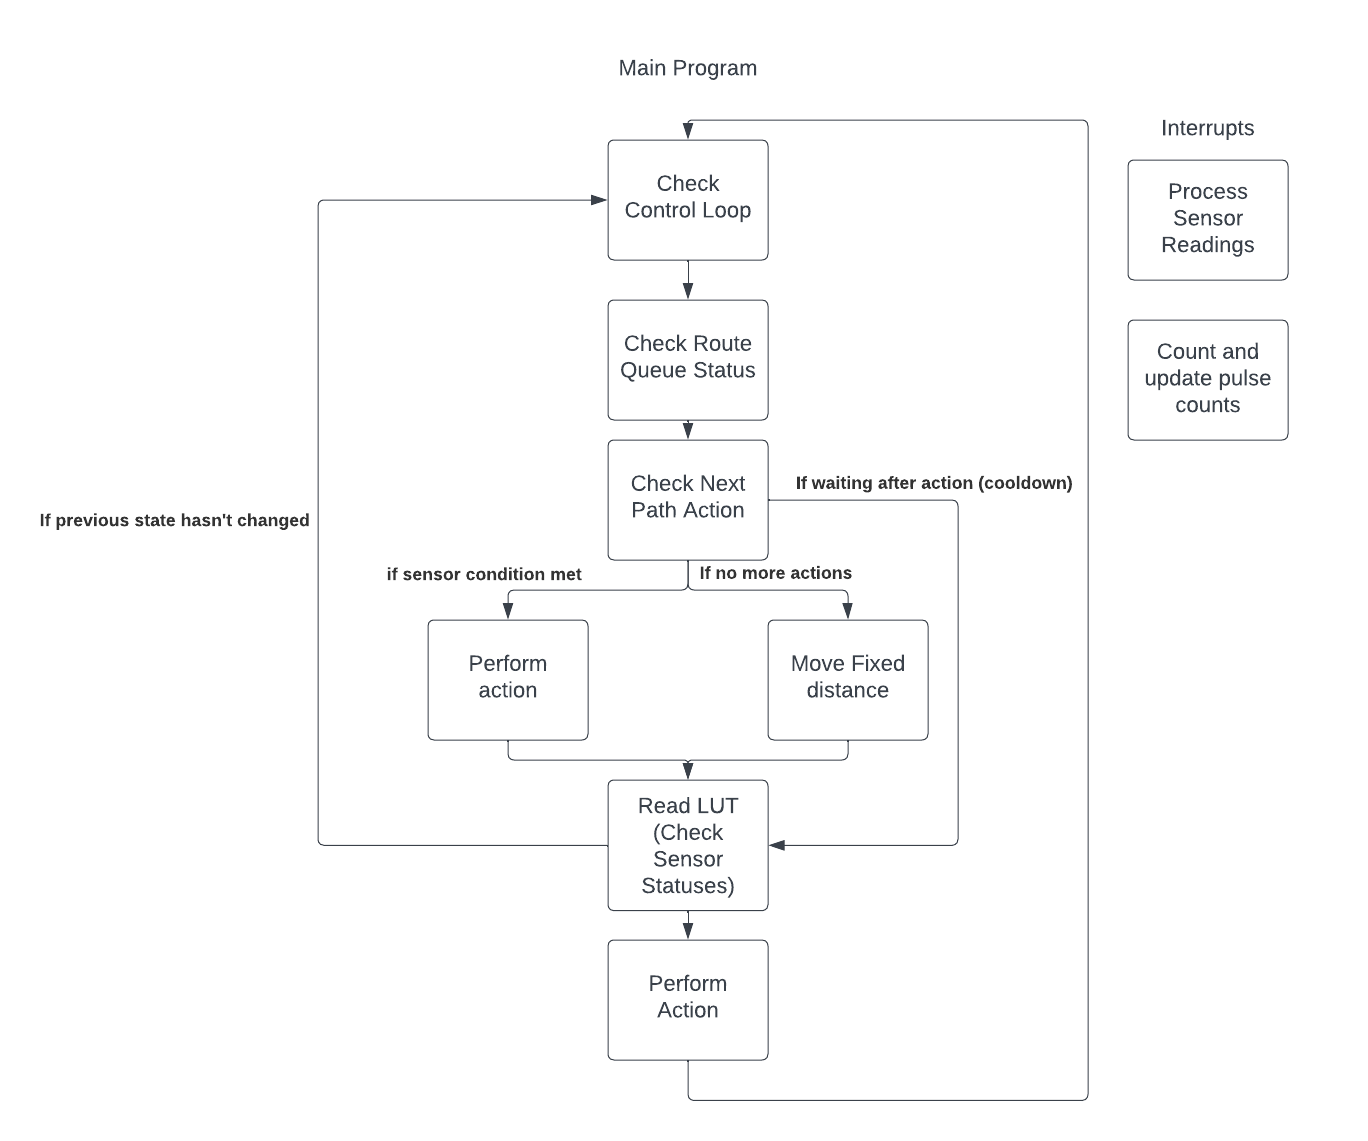
\includegraphics[width=0.5\textwidth]{integration-flowchart.png}}
% 	\caption{Our high-level firmware architecture}
% 	\label{fig:integration-flowchart}
% \end{figure}

\end{document}
